\documentclass[10pt,sigplan,letterpaper,twocolumn]{article}
\usepackage[10pt,nocopyright]{sigmin}

\usepackage{iftex}
\ifXeTeX
  \usepackage{fontspec}
  \usepackage{xeCJK}
  \defaultfontfeatures{Ligatures=TeX}
  \IfFontExistsTF{TeX Gyre Termes}{\setmainfont{TeX Gyre Termes}}{\setmainfont{Times New Roman}}
  \IfFontExistsTF{TeX Gyre Heros}{\setsansfont{TeX Gyre Heros}}{\setsansfont{Arial}}
  \IfFontExistsTF{TeX Gyre Cursor}{\setmonofont{TeX Gyre Cursor}}{\setmonofont{Menlo}}
  \IfFontExistsTF{Songti SC}{
    \setCJKmainfont{Songti SC}[BoldFont=Heiti SC,AutoFakeSlant=0.2]
  }{
    \setCJKmainfont{STSong}[BoldFont=STHeiti,AutoFakeSlant=0.2]
  }
  \IfFontExistsTF{Heiti SC}{\setCJKsansfont{Heiti SC}}{\setCJKsansfont{STHeiti}}
  \IfFontExistsTF{STSong}{\setCJKmonofont{STSong}}{\setCJKmonofont{Songti SC}}
  \XeTeXlinebreaklocale "zh"
  \XeTeXlinebreakskip = 0pt plus 1pt
\else
  \usepackage[T1]{fontenc}
  \usepackage{times}
\fi

\usepackage{listings}
\usepackage{color}
\usepackage{dingbat}
\usepackage[short]{optidef}
\usepackage{epsfig,makecell}
\usepackage[hyphens]{url}
\usepackage[breaklinks,colorlinks]{hyperref}
\hypersetup{citecolor=blue,linkcolor=blue}
\let\burl\url
\usepackage{amsmath,amsopn,amssymb,amsthm}
\usepackage{thmtools}
\usepackage{thmbox}
\usepackage[toc,page]{appendix}
\usepackage{subcaption}
\usepackage{endnotes,microtype,xspace,fancyvrb,multirow}
\usepackage{epigraph}
\usepackage{stfloats}
\usepackage{booktabs}
\usepackage{tabularx}
\usepackage{array,underscore,relsize}
\usepackage{fancyhdr,lastpage}
\usepackage{enumitem}
\usepackage[labelfont=bf,font=normal,skip=1pt]{caption}
\usepackage[export]{adjustbox}
\usepackage{pifont}
\usepackage{tablefootnote}
\usepackage{bbding}
\usepackage[table]{xcolor}
\usepackage[linesnumbered,vlined,boxed,commentsnumbered,ruled]{algorithm2e}
\usepackage{float}
\DontPrintSemicolon
\newcommand{\ra}[1]{\renewcommand{\arraystretch}{#1}}
\newcommand{\nospacestitle}[1]{\noindent{\bf #1}}

\usepackage{amssymb}
\usepackage[normalem]{ulem}
\pagestyle{fancy}
\fancyhf{}
\renewcommand{\headrulewidth}{0pt}
\cfoot{\thepage}

\usepackage[hang,flushmargin]{footmisc}
\usepackage{textcomp}
\usepackage{graphicx}
\usepackage{authblk}
\usepackage[available]{usenixbadges}

\usepackage[compact]{titlesec}
\titleformat*{\section}{\large\bfseries}
\titleformat*{\subsection}{\normalsize\bfseries}
\titleformat*{\subsubsection}{\normalsize\bfseries}
\titlespacing{\section}{0pt}{3ex}{1ex}
\titlespacing{\subsection}{0pt}{2ex}{1ex}

\captionsetup[figure]{labelfont={bf},name={图}}
\captionsetup[table]{labelfont={bf},name={表}}
\renewcommand{\figurename}{图}
\renewcommand{\tablename}{表}
\renewcommand{\abstractname}{摘要}
\renewcommand{\refname}{参考文献}

\lstset{
  basicstyle=\scriptsize,
  tabsize=4,
  frame=single,
  keywordstyle=\bf\color{blue},
  identifierstyle=\bf,
  commentstyle=\it\color[RGB]{0,96,96},
  stringstyle=\rmfamily\slshape\color[RGB]{128,0,0},
  showstringspaces=false
}

\hypersetup{
  colorlinks,
  linkcolor={red!50!black},
  citecolor={blue!50!black},
  urlcolor={blue!80!black}
}

\newtheorem{definition}{定义}
\newtheorem{theorem}{定理}
\hyphenation{para-digms}

\newcommand{\sys}{{\textsc{BlitzScale}}}
\newcommand{\maas}{\textsc{MaaS}}
\newcommand{\blitz}{\textsc{BlitzScale}}
\newcommand{\base}{ServerlessLLM}

\newcommand{\syskv}{{\textsc{Offloaded-KV}}}
\newcommand{\rkv}{{{R-KVS}}}
\newcommand{\drtm}{{{DrTM-KV}}}

\newcommand{\dpu}{{{Bluefield}}}
\newcommand{\snic}{{{SmartNIC}}}
\newcommand{\etal}{\textit{et al}.}
\newcommand{\linefs}{LineFS}
\newcommand{\servingabstraction}{GCG}
\newcommand{\scalingabstraction}{SG}

\newcommand{\fig}[1]{图~\ref{#1}}
\newcommand{\eqa}[1]{公式~\ref{#1}}

\newcommand{\cmark}{\ding{51}}%
\newcommand{\xmark}{\ding{55}}%
\newcommand{\one}{\texttt{\uppercase\expandafter{\romannumeral1}}}
\newcommand{\two}{\texttt{\uppercase\expandafter{\romannumeral2}}}

\newcommand{\wassm}{WebAssembly}

\newcommand{\ssc}[1]{\mbox{\smaller[0.5]{\textsc{{#1}}}}}
\def\ie{即~}
\def\eg{例如~}

\newcommand{\sn}[1]{\mbox{\smaller[0.5]{#1}}}
\newcommand{\cc}[1]{\mbox{\smaller[0.5]\texttt{#1}}}
\newcommand{\ssf}[1]{{\small\textsf{{#1}}}}

\newcommand{\blue}[1]{\textcolor{blue}{#1}}
\newcommand{\red}[1]{\textcolor{red}{#1}}
\newcommand{\hred}[1]{\textcolor[rgb]{0.7,0,0.8}{#1}}
\newcommand{\lred}[1]{\textcolor[rgb]{1,0.3,1}{#1}}

\newcommand{\pcomment}[2]{{\bf[\textcolor{red}{#1}: \textcolor{blue}{#2}]}}
\newcommand{\CR}[1]{{\pcomment{CR}{#1}}}
\newcommand{\XD}[1]{\textcolor{blue}{XD: #1}}
\newcommand{\SSJ}[1]{{\pcomment{SSJ}{#1}}}
\newcommand{\HB}[1]{{\pcomment{CHB}{#1}}}
\newcommand{\tmac}[1]{{\pcomment{tmac}{#1}}}
\newcommand{\YH}[1]{{\pcomment{YH}{#1}}}
\newcommand{\WTX}[1]{{\pcomment{WTX}{#1}}}
\newcommand{\DY}[1]{\textcolor{orange}{DY: #1}}
\newcommand{\TODO}[1]{\textcolor{red}{TODO: #1}}

\newcommand{\revise}[1]{\textcolor{red}{!!!: #1}}
\newcommand{\refine}[1]{\textcolor{blue}{#1}}
\newcommand{\YS}[1]{\textcolor{green}{YS: #1}}

\newcommand{\stitle}[1]{\vspace{1.1ex}\noindent{\bf #1}}
\newcommand{\etitle}[1]{\vspace{0.8ex}\noindent{\em\underline{#1}}}
\newcommand{\eetitle}[1]{\vspace{1ex}\noindent{\em{#1}}}
\newcommand{\sstab}{\rule{0pt}{8pt}\\[-1.8ex]}
\newcommand{\highlight}[1]{\red{\textbf{#1}}}

\usepackage{tikz}
\usepackage{colortbl}
\usetikzlibrary{tikzmark,calc}

\newcommand*\BR[1]{%
\begin{tikzpicture}[baseline=(C.base)]
\node[draw,rectangle,fill=blue,inner sep=1.5pt](C) {\textcolor{white}{#1}};
\end{tikzpicture}}

\usepackage{balance}
\interfootnotelinepenalty=10000

\newcolumntype{P}[1]{>{\centering\arraybackslash}p{#1}}

\definecolor{appcolor}{RGB}{191,255,255}
\newcommand\PartiallyFilledCellWidth[4]{
\tikz[overlay,remember picture]
    \fill[#1] ( $ (pic cs:#2) + (-0.1pt,-0.1pt) $ ) rectangle ++(#4*#3cm - 0.8pt,1.8ex);
}
\newcommand\PartiallyFilledCell[3]{
\tikz[overlay,remember picture]
    \fill[#1] ( $ (pic cs:#2) + (-0.1pt,-0.1pt) $ ) rectangle ++(#3*2cm - 0.8pt,1.8ex);
}

\makeatletter
\renewcommand\AB@affilsepx{ \quad\protect\Affilfont \, }
\renewcommand{\abstract}{
\setcounter{footnote}{0}
\section*{摘要}\normalsize
}
\renewcommand{\endabstract}{\if@twocolumn\else\endquotation\fi}
\makeatother

\SetKwInput{KwInput}{输入}
\SetKwInput{KwOutput}{输出}
\SetKwComment{Comment}{$\triangleright$\ }{}

\begin{document}

\title{\Large \bf{{\textsc{BlitzScale}}：基于 $O(1)$ 主机缓存的大模型快速在线自动扩缩容}}

\setlength{\affilsep}{0.5em}
\author[1]{Dingyan Zhang, Haotian Wang$^\dagger$, Yang Liu$^\dagger$, Xingda Wei\,{\Envelope}}
\author[2]{Yizhou Shan}
\author[1]{Rong Chen, Haibo Chen}

\affil[1]{\vspace{-2.mm}上海交通大学并行与分布式系统研究所}
\affil[2]{华为云\vspace{-1.mm}}

\date{}
\maketitle
\def\thefootnote{$\dagger$}\footnotetext{以上作者贡献相同。}
\def\thefootnote{\Envelope}\footnotetext{通讯作者：Xingda Wei（\texttt{wxdwfc@sjtu.edu.cn}）。}
\def\thefootnote{}\footnotetext{发表于第 19 届 OSDI Conference，Boston, MA, USA，2025。}

\renewcommand{\thefootnote}{\arabic{footnote}}

\frenchspacing

\begin{abstract}
\noindent
模型自动扩缩容是实现无服务器模型即服务的关键机制，
但它在扩缩速度与用于缓存参数的存储/内存占用之间存在根本性权衡，
因而难以满足跨多主机、频繁发生的扩容需求。
核心问题在于数据平面过慢：
在参数加载完成之前，新扩出的实例始终处于停机状态。

本文首先指出，如果通过 GPU 之间的计算网络加载参数，
那么即使完全不依赖缓存或仅使用 $O(1)$ 缓存，
也能让数据平面变得\emph{快速}，原因在于：
(1) 该路径的速度与主机缓存相当，却长期未被充分利用；
(2) 借助针对网络优化的多播，扩多个实例时仍只需要零或 $O(1)$ 缓存。
其次，我们通过将推理扩缩容的抽象从粗粒度的实例级下沉到细粒度的层级，
使自动扩缩容变得\emph{在线}。
这样一来，无需等待参数全部加载完成，
就可以把过载服务实例中的部分层计算卸载到新扩出的实例上。

在真实工作负载下，
我们的系统 {\sys} 相比最先进的自动扩缩容系统 ServerlessLLM，
最多可将尾延迟降低 94\,\%；
而与不支持自动扩缩容、但满足相同服务等级协议的 DistServe 与 vLLM 相比，
{\sys} 可将服务所消耗的 GPU 时间降低 49\,\%。
\end{abstract}

\section{引言}
\label{sec:intro}

\noindent
近年来，以大语言模型（LLM）为代表的深度学习模型正在快速推动各类应用的发展~\cite{aws-rekognition,chatgpt,copilot,sora,stability-ai}。
由于这类模型的计算需求极其庞大，
它们通常以模型即服务（model-serving-as-a-service，{\maas}）系统的形式对外提供能力~\cite{serverless-together-ai,serverless-ray,deepinfra,DBLP:conf/asplos/YangZLZLZCL22,ali-serverless-llm,aws-serverless-llm,DBLP:journals/corr/abs-2401-14351}。
这类系统统一管理一个由加速器（例如 GPU）组成的集群，
并为每个已部署模型分配适量的服务\emph{实例}，
每个实例都包含用于执行推理的 GPU 资源。

{\maas} 系统有两个核心设计目标：
一是\emph{最大化 goodput}——也就是满足服务等级目标（SLO）的请求数量；
二是\emph{最小化分配给每个模型的实例数量}，以提升硬件利用率。
要同时满足这两个目标并不容易，
因为单个模型对实例数量的短期需求会发生难以预测的波动：
请求到达率可能在秒级突增，在 2 秒内增长 5\,$\times$~\cite{alpaserve,DBLP:conf/nsdi/0025TKS23}；
与此同时，由于 LLM 具有自回归特性，
单个请求带来的内存占用同样难以预估~\cite{alpaserve,DBLP:conf/nsdi/0025TKS23,DBLP:journals/corr/abs-2401-14351}。
关于这一点，可参见 {\fig{fig:problem-statement}} 与 \textsection{\ref{sec:problem-statement}}。

模型自动扩缩容是一种很有前景的解决方案~\cite{DBLP:conf/asplos/YangZLZLZCL22,serverless-ray,DBLP:journals/corr/abs-2401-14351,kserve}。
借助自动扩缩容，
{\maas} 系统只需为每个模型长期维持其平均所需的实例数量，
而这一平均需求通常相对稳定~\cite{wang2024burstgpt}，
因此能够提升整体利用率。
当突发流量出现时，
系统再自动扩出新的实例，
以避免由于已分配实例不足、请求排队过长而造成的 SLO 违约。

自动扩缩容的速度对于减少 SLO 违约至关重要，
因为在扩出的实例可用之前，排队请求都无法得到处理。
以 Llama3-8B 为例，
它在商用 GPU（A800）上的单次推理时间约为 80--900\,ms，
而在聊天机器人等场景中，用户通常期望响应时间低于 1 秒~\cite{latency-study,DBLP:conf/osdi/ZhongLCHZL0024,aws-latency}。
为了满足这样的严格 SLO，
扩缩容时间通常必须低于 500\,ms。
然而，对于参数规模达到 10--400\,GB 的 LLM 来说，实现这一点非常困难。
根本原因在于自动扩缩容的\textbf{数据平面过慢}——也就是把模型参数加载到实例 GPU 上的过程过慢。
现有工作虽然已经利用高带宽 SSD 来加速这一过程~\cite{DBLP:journals/corr/abs-2401-14351}，
但 GPU 服务器上的 SSD 所能提供的速度（每 GPU 仅 2--10\,Gbps~\cite{googleinstance,awsinstance,volcanoinstance}）仍远远不够。
例如，在 10\,Gbps SSD 上把 Llama3-8B 加载到一张 GPU 上，需要 12.8 秒。
另一个阻碍快速扩缩容的因素是，现有方法大多是\textbf{stop-the-world} 的：
在所有参数完成加载之前，新扩出的实例无法处理任何请求。
这意味着自动扩缩容的速度会被数据平面直接卡住。

为缓解上述问题，ServerlessLLM 等最先进系统进一步采用了多级缓存，
把模型参数缓存在主机（CPU）内存中，以加速数据平面~\cite{DBLP:conf/osdi/GujaratiKAHKVM20,DBLP:conf/eurosys/JeongBA23}。
在缓存命中的情况下，
系统可以借助高速 CPU-GPU 链路（例如 256\,Gbps 的 PCIe）来加载参数。
然而，想要获得很高的命中率并不现实：
ServerlessLLM 报告的缓存命中率只有 40--75\,\%，
我们的实验也验证了这一点（见 \textsection{\ref{sec:bg-motiv}}）。
根本原因在于，{\maas} 系统一般会同时托管大量模型，
而若想在每台主机的 DRAM 中都缓存这些模型、从而达到 100\,\% 命中率，显然并不现实。
云厂商之所以需要托管如此多模型，
是因为当下存在数百个面向不同用途的热门开源模型家族~\cite{huggingface}；
同时，每个模型家族内部通常还有多个规模版本，
用于在精度与服务成本之间进行权衡~\cite{qwens}。
此外，开发者还可以基于开源模型上传自己微调后的定制版本~\cite{aws-serverless-llm}。

为了在不依赖缓存命中的前提下实现快速模型扩缩容，
我们做出了以下两点关键贡献：

\stitle{1. 借助计算网络多播，在 $O(1)$ 或零缓存下实现快速数据平面。\,}
首先，{\maas} 系统通常依赖高速 GPU-GPU/CPU 计算互连~\cite{nvidia-compute-network}，
其带宽可达 100--400\,Gbps 的 RDMA，甚至 16\,Tbps 的 NVLink~\cite{googleinstance,awsinstance,volcanoinstance}，
明显快于 SSD，也与 CPU-GPU PCIe 相当，甚至更快。
这些计算网络本来就会在推理过程中承担数据传输，
但我们发现它们普遍处于低利用状态：
即使在采用 Prefill/Decode 解耦的网络密集型 LLM 服务负载中，
其总带宽利用率也只有 7.4\,\% 左右~\cite{DBLP:conf/isca/PatelCZSGMB24, DBLP:conf/osdi/ZhongLCHZL0024,DBLP:journals/corr/abs-2401-11181,DBLP:conf/ppopp/CaiLMMMNS21,DBLP:journals/corr/abs-2404-09526}（见 \textsection{\ref{sec:bg-motiv}}）。
因此，我们可以把这些高速链路借来加速自动扩缩容的数据平面。

其次，基于网络的数据平面只需要极少甚至不需要缓存就能实现快速扩缩容。
具体来说，
如果某个模型已经部署在若干实例上，
我们就可以直接通过网络把这些已部署实例中的参数多播出去，
从而完全不依赖缓存。
这种多播之所以高效，
是因为串行转发式多播~\cite{DBLP:conf/icpp/VerstoepLB96}
在传输大块数据（例如模型参数）时，
其开销基本与接收端数量无关。
即使某个模型当前还没有任何已部署实例，
我们也只需要在某台主机上缓存一份参数，
然后由该主机进行广播，即可在 $O(1)$ 主机缓存下完成多播。
这种“每个模型只需 $O(1)$ 缓存副本”的方式，
使我们能够避免缓存未命中，
因为整个集群的主机总内存足以缓存 {\maas} 所服务的全部模型。

尽管高速网络能够在极少缓存的前提下显著加快数据平面，
但只要扩缩容仍是 stop-the-world，
在网络速度仍不足够快的情况下，它依然会成为瓶颈。
例如，对于 Qwen2.5-72B 在 BurstGPT 工作负载上的服务，
若希望将 SLO 违约率压到 40\,\% 以下，
系统需要把停顿时间控制在 500\,ms 以内。
这意味着每张 GPU 至少需要 576\,Gbps 的参数传输带宽\footnote{\footnotesize{72\,B 模型的单个服务实例至少需要 4 张 GPU。}}，
这不仅超过了典型计算网络配置（例如每 GPU 200\,Gbps）所能提供的带宽，
甚至也超过了主机缓存场景下的 256\,Gbps PCIe。
因此，我们认为理想的参数加载过程必须是\emph{在线}的：
在数据尚未全部加载完成之前，新扩出的实例就应该能够参与服务。

\stitle{2. 借助细粒度扩缩抽象与协同执行，实现在线数据平面。\,}
在传统服务器无状态计算中常见的按需数据加载技术~\cite{mitosis,DBLP:conf/eurosys/WangHW19,DBLP:conf/sosp/HuangZMLLCJLSZL24}，
以及 PipeSwitch~\cite{pipeswitch} 中的推理与加载重叠方法（见 \textsection{\ref{sec:overview}}），
都无法让模型扩缩容真正做到在线。
原因在于，实例只有在所有参数都加载完成之后才能输出最终结果。
这种“必须全部加载完再服务”的停顿，根源在于现有系统采用了粗粒度的实例级扩缩抽象：
它们只能在实例级别完成扩缩和服务。
为了实现在线扩缩容，
我们的核心洞察是：\emph{模型可以按照逐层的细粒度方式进行服务}。
在这种逐层扩缩抽象下，
我们可以把部分层的计算从过载实例卸载到新扩出的实例上，
通过协同执行的方式，
在新实例尚未加载完全部参数之前就提升整体服务吞吐。

\stitle{挑战与解决方案。\,}
首先，在我们的场景中利用基于网络的多播并不容易。
虽然多播机制本身很直接——也就是简单地通过网络在实例之间转发参数——
但难点在于如何生成多播计划，
也就是决定数据应当如何在实例之间流动。
一方面，源和目标会动态变化，
而服务集群中的异构网络上求解最优计划是 NP-hard 的~\cite{DBLP:journals/jpdc/BhatRP03}；
另一方面，我们还必须避免扩缩容流量与在线服务流量相互干扰，
否则我们观察到扩缩时间会延长 1.5\,$\times$，尾部 TBT 下降 50\,\%（见 \textsection{\ref{sec:overview}}）。
现有方案~\cite{DBLP:conf/asplos/CowanMMSX23,DBLP:conf/ppopp/CaiLMMMNS21,DBLP:conf/sc/GhazimirsaeedZR20}
主要面向训练等离线场景，
可以容忍较长的计划生成时间，
也无须考虑与服务工作负载之间的干扰。
为此，我们提出了一个面向模型的多播规划器，
利用计算网络的关键特性以及模型服务中静态的数据流模式，
快速生成近似最优且无干扰的扩缩容多播计划（见 \textsection{\ref{sec:design-plan}}）。

其次，如何在已部署实例与在线扩缩实例之间调度请求执行也很有挑战，
也就是决定每个实例执行哪些层。
困难在于，扩缩中的新实例服务能力是受限的：
它只能执行那些对应参数已经加载完成的层，
而且这种能力会持续变化。
一个朴素的“尽力而为”方案是让新实例能执行多少层就执行多少层，
但这无法平衡负载，
因为在扩缩早期，新实例只能执行极少数层，
大多数请求仍会积压在过载实例上。
更好的办法是从全局角度考虑后续将到来的层，
并据此动态平衡负载。
我们通过 ZigZag 流水线调度来实现这一点，
在突发负载下可将尾延迟降低 50\,\%（见 \textsection{\ref{sec:design-pp}}）。

\stitle{{\sys} 的实现与验证。\,}
我们实现了 {\sys}，
这是一个只需 $O(1)$ 缓存、同时具备极快自动扩缩容速度的 {\maas} 系统。
我们在系统中引入了跨机器的全局参数池，
并集成了上述无干扰多播扩缩计划以及基于 ZigZag 调度的在线执行机制。
为了验证 {\sys} 的有效性，
我们在多个真实工作负载轨迹上进行了评估，
包括 BurstGPT~\cite{wang2024burstgpt}、AzureCode 与 AzureConv~\cite{AzurePublicDataset}，
并覆盖了多种不同规模、不同结构的近期模型，
包括 Llama3-8B、Mistral-24B 和 Qwen2.5-72B。
结果表明：
第一，相比当前最先进的 ServerlessLLM~\cite{DBLP:journals/corr/abs-2401-14351}，
{\sys} 的首 token 时间（TTFT）缩短了 47--75\,\%，
token 间时间（TBT）最多缩短了 94\,\%；
第二，与不支持自动扩缩容的 vLLM~\cite{vllm} 与 DistServe~\cite{DBLP:conf/osdi/ZhongLCHZL0024} 相比，
在不发生 SLO 违约的前提下，
{\sys} 可将服务单个模型所需的 GPU 数量减少 49\,\%，
这一结果以“按峰值请求率进行过度预配”的配置为参照。
{\sys} 已在 \url{https://github.com/blitz-serving/blitz-scale} 开源。

\section{背景：{\maas} 与自动扩缩容}
\label{sec:bg}

\subsection{系统设置：模型即服务（\maas）}
\label{sec:model}

\begin{figure*}[!t]
    \centering
    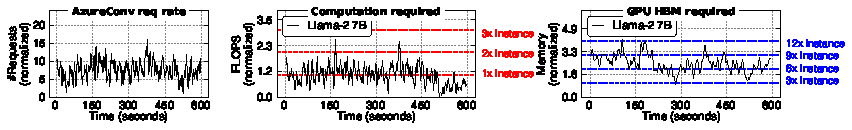
\includegraphics[width=1.01\textwidth,center]{./data/problem/scripts/problem.pdf} \\[0pt]
    \begin{minipage}{1\linewidth}
    \caption{\small{\textit{
        真实 AzureConv~\cite{AzurePublicDataset} 轨迹的请求到达率时间线（a），
        以及在无 SLO 违约条件下服务该工作负载所需的计算资源（b）与内存资源（c）。
    }}}
    \label{fig:problem-statement}
    \end{minipage} \\[-15pt]
\end{figure*}

\begin{figure}[!t]
    \begin{minipage}{1\linewidth}
        \hspace{-1mm}
        \centering
        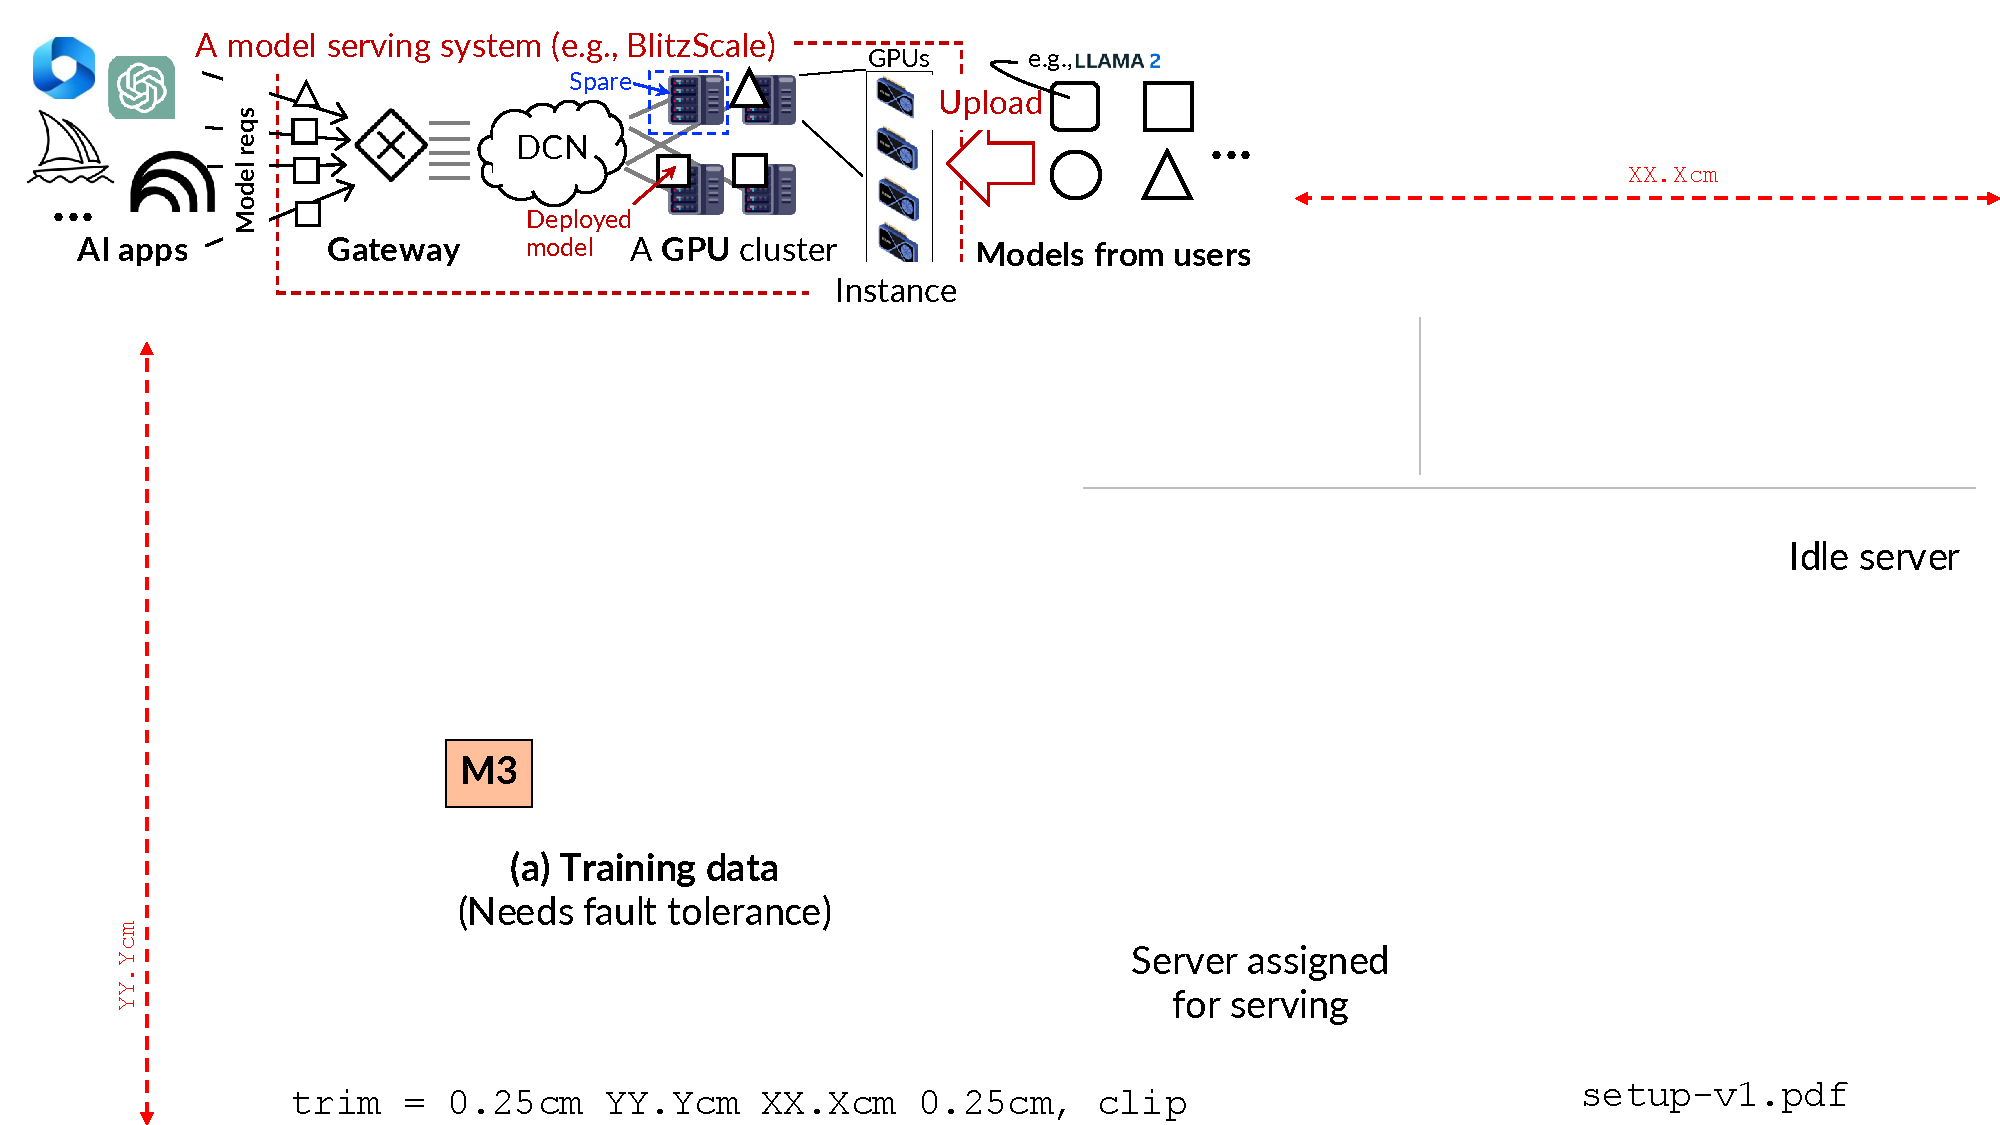
\includegraphics[width=\columnwidth, trim=0.25cm 13.8cm 12cm 0.25cm, clip]{figs/setup-v1.pdf} \\[1pt]
    \end{minipage} \\[3pt]
    \begin{minipage}{1\linewidth}
        \caption{\small{\textit{
            模型即服务（{\maas}）系统示意图。
            其中 DCN 表示数据中心网络（data center network）。
        }}}
        \label{fig:setup}
    \end{minipage} \\[-20pt]
\end{figure}

\nospacestitle{{\maas} 系统设置与服务实例。\,}
{\sys} 面向 {\maas} 场景~\cite{serverless-together-ai,serverless-ray,deepinfra,DBLP:conf/asplos/YangZLZLZCL22,ali-serverless-llm,aws-serverless-llm,DBLP:journals/corr/abs-2401-14351}：
云平台允许用户把模型部署到其托管硬件上进行服务，
并仅按满足 SLO 的请求数量向用户计费~\cite{aws-serverless-llm,ali-serverless-llm}。
这些模型既可以是 Qwen~\cite{qwens} 这样的热门开源模型，
也可以是用户自行上传的定制模型。
得益于这种计费方式，
云平台可以针对特定模型动态调整硬件资源，
以尽可能提高整体硬件利用率。
{\fig{fig:setup}} 展示了一个典型 {\maas} 系统的部署方式。
对于每个用户部署的模型，
系统会动态分配所需的 GPU 资源来处理其推理请求。
需要注意的是，由于 AI 应用种类繁多，
一个 {\maas} 系统往往会同时服务数百甚至数千个模型~\cite{alibailian}。

在本文中，
我们用 \emph{instance} 表示一组 GPU，
它们共同存放模型参数的完整副本，并用于服务该模型。
当模型较小时，一个实例只需要一张 GPU；
当模型较大、参数需要跨多张 GPU 切分时，
一个实例也可能包含多张 GPU，例如采用张量并行~\cite{narayanan2021efficient}。
由于单个实例的服务吞吐存在上限，
云平台通常会为同一个模型部署多个实例，
即分配多组 GPU 共同服务，
并根据请求到达率动态调整实例数量。
{\sys} 能够与现有各种实例级模型服务方法兼容，并为它们提供自动扩缩容支持。

\stitle{实例内服务：非 LLM 与 LLM。\,}
每个服务实例的基本处理流程如下：
它按照逐层计算的方式查询模型（见 {\fig{fig:overview}} (a)），
并最终得到输出结果。
对于视觉模型等简单模型，
用户只需用输入数据（例如图像）查询模型一次即可。
而对于大语言模型（LLM）~\cite{DBLP:conf/nips/VaswaniSPUJGKP17}，
一次请求需要多次查询模型。
模型首先接收输入文本（prompt）并生成第一个结果 token，
这一阶段通常称为 \emph{prefill}。
随后，模型会基于已生成 token 迭代地产生后续 token，
直到返回终止标记；
这个自回归阶段称为 \emph{decode}。

我们强调 LLM 的两个重要特性。
第一，prefill 与 decode 的性能通常分开衡量：
prefill 采用首 token 时间（TTFT）指标，
decode 采用 token 间时间（TBT）指标。
第二，LLM 查询具有状态性：
在请求的自回归阶段，中间结果——通常称为 \emph{KVCache}——会被保存在 GPU 显存中，以加速后续计算。

\stitle{跨实例服务：Prefill/Decode 解耦的 LLM 服务。\,}
观察到 prefill 与 decode 在计算模式上存在明显差异后，
近期工作提出把负责 prefill 与 decode 的实例分离（即 PD disaggregation），
从而处理服务请求~\cite{DBLP:conf/isca/PatelCZSGMB24, DBLP:conf/osdi/ZhongLCHZL0024,DBLP:journals/corr/abs-2401-11181}。
具体而言，对于每个请求，
由一个实例负责 prefill 阶段（prefill instance），
另一个实例负责 decode 阶段（decode instance）。
这种方式需要在两个实例之间搬运大量数据，
因为 prefill 实例必须把 KVCache 传给 decode 实例。
{\sys} 同时支持 PD 解耦和非解耦两类 LLM 服务方式。

\subsection{服务单个模型时的动态硬件需求}
\label{sec:problem-statement}

\noindent
为一个模型确定合适的硬件配置——也就是确定所需实例数量——并不容易，
因为硬件需求既难以预测，又会持续波动。
首先，服务工作负载中的请求到达率会随时间变化，
而且通常难以预测~\cite{DBLP:journals/corr/abs-2401-14351,DBLP:conf/usenix/ShahradFGCBCLTR20,DBLP:conf/nsdi/0025TKS23}。
{\fig{fig:problem-statement}} (a) 展示了真实轨迹中某个单模型服务的请求数时间线——BurstGPT~\cite{wang2024burstgpt}：
在没有明显规律的情况下，
进入系统的推理请求可以在 2 秒内增长 5\,$\times$。
由于单个实例的 FLOPS 是固定的，
这种难以预测的到达率波动会导致所需计算资源——也就是在 SLO 内完成待处理请求所需的 FLOPS——同样变得不可预测。
{\fig{fig:problem-statement}} (b) 通过测量 Llama2-7B 在 BurstGPT 上服务时 prefill 实例的需求，
验证了这一点。

其次，现代模型（尤其是 LLM）服务还会带来复杂且不可预测的显存需求。
如 {\fig{fig:problem-statement}} (c) 所示，
当使用 Llama2-7B 服务 BurstGPT 时，
decode 实例上的 KVCache 占用会达到单个实例显存容量的数倍，
并随时间在 3--12\,$\times$ 之间波动。
根本原因在于，
请求的 KVCache 必须在 decode 阶段常驻于 GPU 显存中。
这些 KVCache 非常大，
例如在 Llama2-7B 服务 BurstGPT 时可达到 190--760\,GB，
而且由于 LLM 的自回归特性，请求在系统中的停留时间也不可预测。
为了避免内存不足带来的性能损失，
{\maas} 系统必须分配足够多的实例来容纳正在执行请求的 KVCache，
因此，一个模型所需的实例数量也会出现不可预测的波动。

\subsection{用于处理动态需求的模型自动扩缩容}

\noindent
模型自动扩缩容会在空闲 GPU 上动态部署\footnote{\footnotesize{系统也会通过停止服务实例来缩容。由于缩容相对简单，本文不再展开。}}
新的服务实例，从而提升服务能力；
这被认为是应对计算与内存需求波动的一个有前景方案~\cite{DBLP:journals/corr/abs-2401-14351,DBLP:conf/asplos/YangZLZLZCL22,serverless-ray}。
其基本逻辑在于：
单个模型的工作负载虽然难以预测，
但平台上所有模型负载叠加后的总体需求通常更平稳~\cite{DBLP:conf/nsdi/0025TKS23}。
因此，当某个模型的服务负载上升时，
系统能够从其他模型那里回收空闲 GPU，
再将其用于扩容该模型。

扩出一个实例通常包含两个基本步骤：
(1) 初始化合适的执行上下文，例如创建 CUDA 上下文（控制平面）；
(2) 把模型参数加载到 GPU 显存中（数据平面）。
本文主要关注步骤 (2)，
因为步骤 (1) 已经可以通过近期 GPU 启动优化方法（例如 checkpoint/restore）~\cite{DBLP:journals/corr/abs-2405-12079,DBLP:conf/asplos/ZengXGCL25}
以及我们基于 Rust/C++ 的服务框架显著压缩（也见 \textsection{\ref{sec:eval-ablation}}）。
对于步骤 (2)，
当前最先进系统 ServerlessLLM~\cite{DBLP:journals/corr/abs-2401-14351}
通过面向 SSD 的参数加载优化了数据平面。
但它并没有从模型服务对扩缩速度的要求出发进行设计。
下一节中的测量结果表明，
基于 SSD 的扩缩速度仍然明显落后于实际应用需求。

\begin{figure*}[!t]
    \centering
    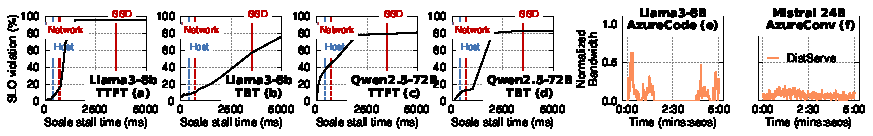
\includegraphics[width=1.01\textwidth,center]{./data/motiv-slo-all.pdf} \\[2pt]
    \begin{minipage}{1\linewidth}
    \caption{\small{\textit{
        在 BurstGPT~\cite{wang2024burstgpt} 上，不同推理场景 (a)--(d) 在不同自动扩缩停顿时间下的 SLO 达成情况；
        (e) 与 (f) 则分析了服务工作负载中的计算网络使用情况。
        评测设置见 \textsection{\ref{sec:eval}}。
    }}}
    \label{fig:motiv-scale-speed}
    \end{minipage} \\[-5pt]
\end{figure*}

\section{实例间扩缩容需求与计算网络特征分析}
\label{sec:bg-motiv}

\nospacestitle{模型自动扩缩容需要快速数据平面。\,}
如果数据平面的速度不够快，
那么在突发期间，
请求仍会因为排队时间变长而违反 SLO。
这里的 SLO 指的是端到端时延约束，
即从请求发出到推理结果返回的总耗时。
因此，这一时延自然也包含了等待新扩出实例就绪所产生的排队延迟。

为了刻画不同扩缩速度对 SLO 达成率的影响，
我们在 DistServe~\cite{DBLP:conf/osdi/ZhongLCHZL0024} 上实现了一个模拟器：
该模拟器把模型预先部署到所有 GPU 上，
然后通过人为插入延迟来模拟不同的数据平面速度。
TTFT 与 TBT 的 SLO 设置遵循已有工作~\cite{DBLP:conf/osdi/ZhongLCHZL0024} 中不同模型的推理速度。
具体来说，
对于 Llama3-8B，我们采用 450\,ms 的 TTFT SLO 和 150\,ms 的 TBT SLO；
对于张量并行度为 4 的 Qwen2.5-72B，我们采用 1250\,ms 的 TTFT SLO 和 200\,ms 的 TBT SLO。
更详细的评测设置见 \textsection{\ref{sec:eval}}。

{\fig{fig:motiv-scale-speed}} (a)--(d) 展示了结果。
可以看到，
对于 72\,B 模型，
若想把 SLO 违约率控制在 60\,\% 以下，
单个实例、每张 GPU 至少需要 220\,Gbps 的扩缩速度\footnote{\footnotesize{72\,B 模型的单个实例使用 4 张 GPU。}}；
而这一速度只有在模型参数从主机内存加载时才能达到。
扩缩时间需求与推理时间直接相关——我们评测的 BurstGPT~\cite{wang2024burstgpt}
工作负载平均 TTFT（含排队）为 771\,ms。
因此，如果要让所有请求都满足 1250\,ms SLO，
扩缩时间必须低于 500\,ms，
也就要求每张 GPU 具备 576\,Gbps 的网络速度
（通过参数规模除以扩缩时间得到）。
这一要求远超厂商提供的每 GPU SSD 带宽（2--10\,Gbps~\cite{googleinstance,awsinstance,volcanoinstance}；详见 \textsection{\ref{sec:appendix-hardware}}）。

\begin{figure}[!t]
    \centering
    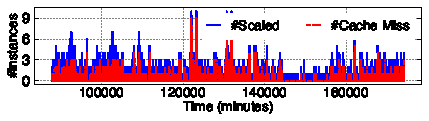
\includegraphics[width=1.01\linewidth,center]{./data/motiv-cache-miss.pdf} \\[1pt]
    \begin{minipage}{1\linewidth}
    \caption{\textit{\small{
        在 BurstGPT~\cite{wang2024burstgpt} 上运行 ServerlessLLM~\cite{DBLP:journals/corr/abs-2401-14351} 时主机缓存未命中的分析。
    }}}
    \label{fig:motiv-cache-miss}
    \end{minipage} \\[-5pt]
\end{figure}

\stitle{从主机内存加载模型参数并不总是有效，因为未命中很常见。\,}
当 CPU 主机内存中缓存了参数时，
借助高速 Host-GPU 互连（例如 256\,Gbps PCIe 4.0），
某些配置（如 8\,B、24\,B）确实能够满足扩缩速度要求。
但是在真实轨迹中，缓存未命中非常常见，
因为有限的主机内存无法支持把 {\maas} 系统中部署的所有模型都缓存下来。
{\fig{fig:motiv-cache-miss}} 展示了在 BurstGPT 工作负载下使用 ServerlessLLM~\cite{DBLP:journals/corr/abs-2401-14351} 时，
扩出的实例数量以及遭遇的缓存未命中情况。
按照其原始设置，
我们将主机缓存的 keep-alive 时间设置为 5 分钟。
可以看到，缓存未命中率会随时间在 20--46\,\% 之间波动，
与 ServerlessLLM 论文中报告的 25--60\,\% 基本一致。
有趣的是，许多未命中发生在需要同时扩多个实例时，
因为涉及主机越多，
在没有缓存该模型参数的主机上扩容的概率就越高。
因此，即使主机缓存未命中，
我们仍然需要找到办法加快扩缩速度。

\begin{figure}[!t]
    \begin{minipage}{1\linewidth}
        \hspace{-1mm}
        \centering
        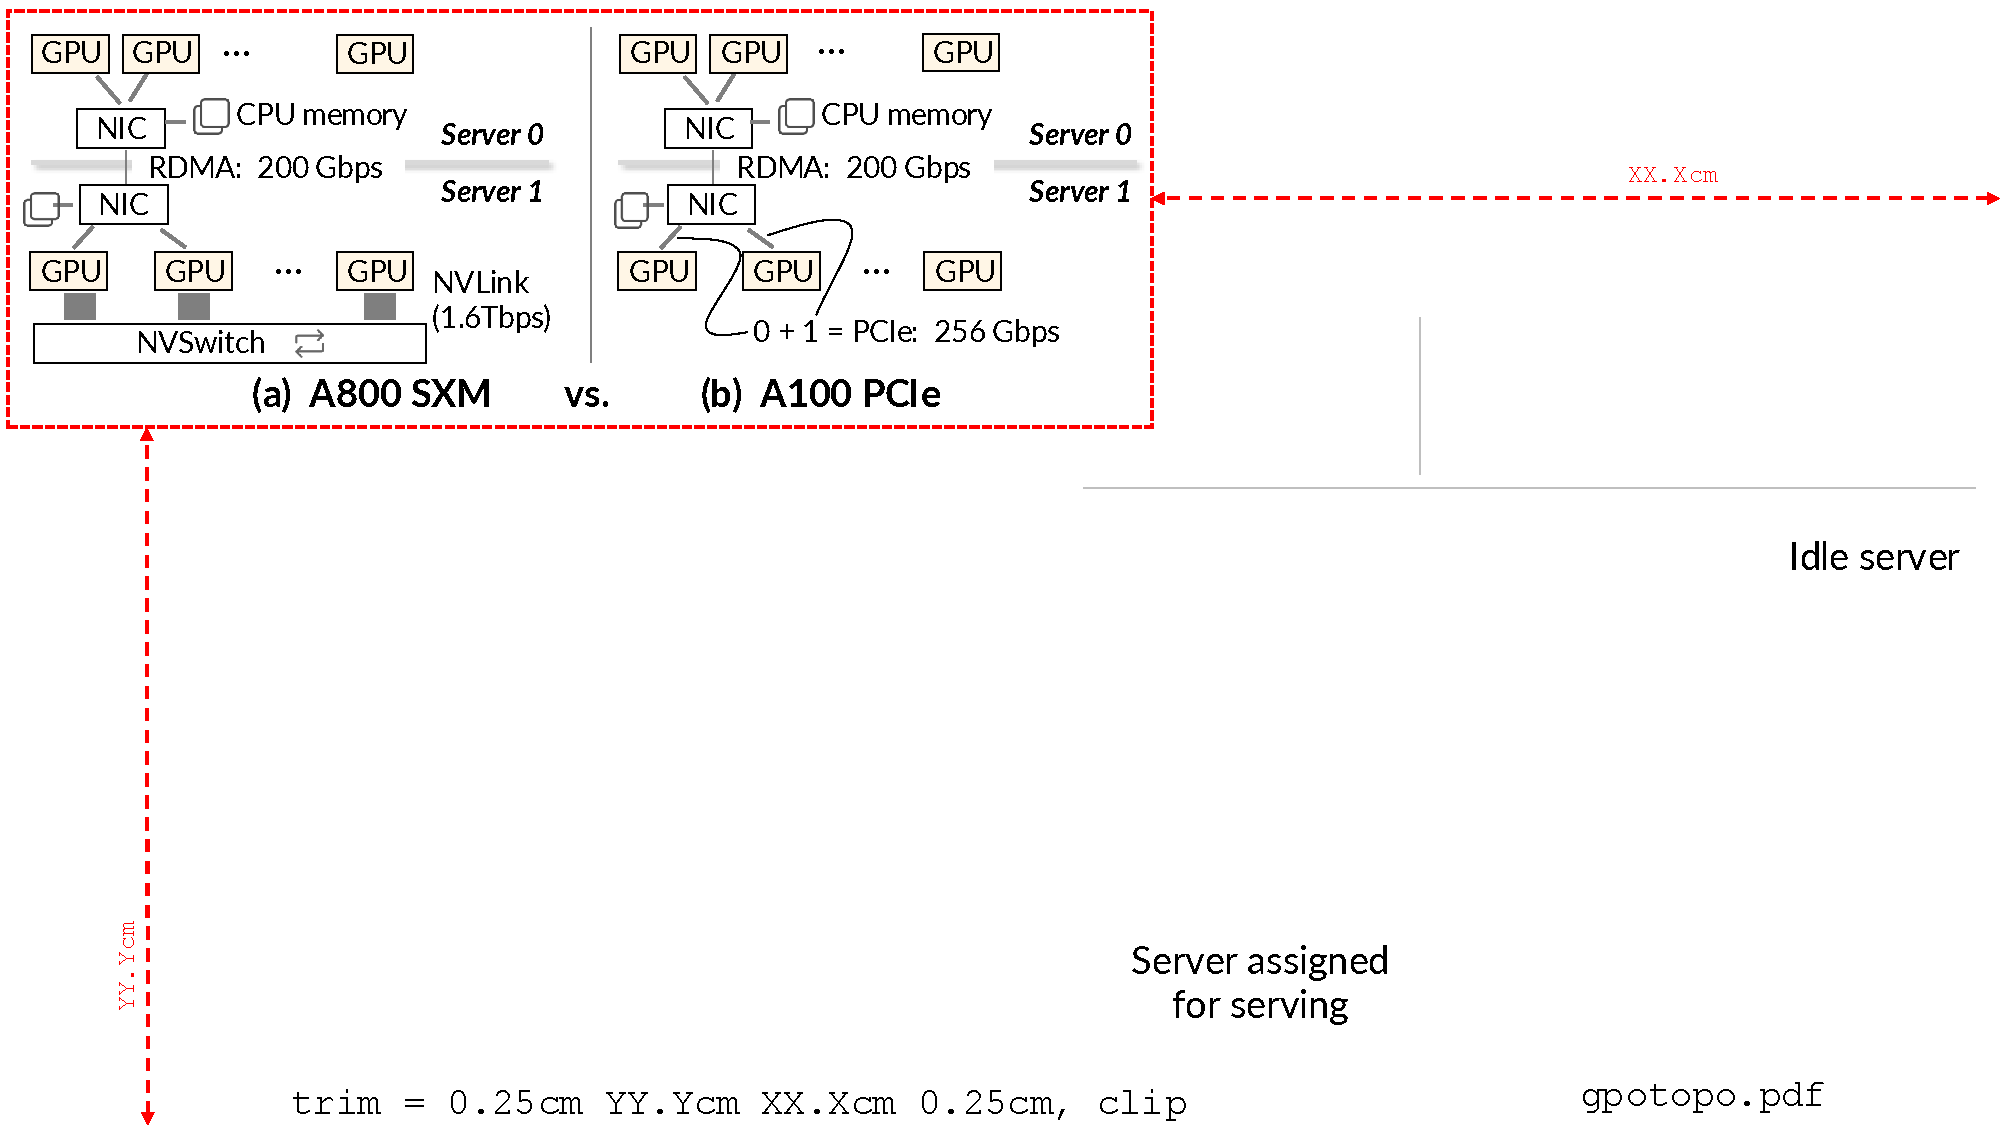
\includegraphics[width=.99\textwidth, trim=0.25cm 11.9cm 14.4cm 0.25cm, clip]{figs/gputopo.pdf} \\[1pt]
    \end{minipage} \\[4pt]
    \begin{minipage}{1\linewidth}
        \caption{\textit{\small{
            带 NVLink（a）与不带 NVLink（b）时，{\maas} 中网络连接方式的示意图。
            注意，一条 256\,Gbps 的 PCIe 链路会被其连接的两张 GPU 共享~\cite{nvidia-all-to-all}。
        }}}
        \label{fig:gputopo}
    \end{minipage} \\[-10pt]
\end{figure}

\stitle{机会：高速且低利用率的计算网络。\,}
首先，GPU（以及 CPU）之间的计算网络速度可与 Host-to-GPU 链路相当，甚至更快。
如 {\fig{fig:gputopo}} 所示，
GPU 间网络（RDMA）的速率可达 200\,Gbps，
已经接近 Host-GPU PCIe 的 256\,Gbps；
而在有 NVLink 时，速度则更高。
更重要的是，
这些网络在服务过程中通常没有被充分利用。
{\fig{fig:motiv-scale-speed}} (e) 与 (f) 测量了 DistServe~\cite{DBLP:conf/osdi/ZhongLCHZL0024} 的峰值网络使用情况。
DistServe 是一个采用 PD 解耦的服务系统，
由于需要搬运 KVCache，因此本身就高度依赖网络。
为了测量峰值用量，
我们把所有 GPU 都用于服务，
并在集群可承受的最大请求率下执行工作负载。
结果表明，即使在峰值负载下，
仍有超过 40\,\% 的网络容量处于空闲状态，
这为利用计算网络承载扩缩容数据平面提供了机会。

\section{{\sys} 系统概览}
\label{sec:overview}

\definecolor{boxcolor}{HTML}{FFFFFF}
\definecolor{boxcolortwo}{HTML}{FFF6E6}

\newcommand{\fboxone}[1][1em]{%
  \tikz\filldraw[fill=boxcolor,draw=black] (0,0) rectangle (#1,#1);
}

\newcommand{\fboxtwo}[1][1em]{%
  \tikz\filldraw[fill=boxcolortwo,draw=black] (0,0) rectangle (#1,#1);
}

\begin{figure}[!t]
    \begin{minipage}{1\linewidth}
        \hspace{-1mm}
        \centering
        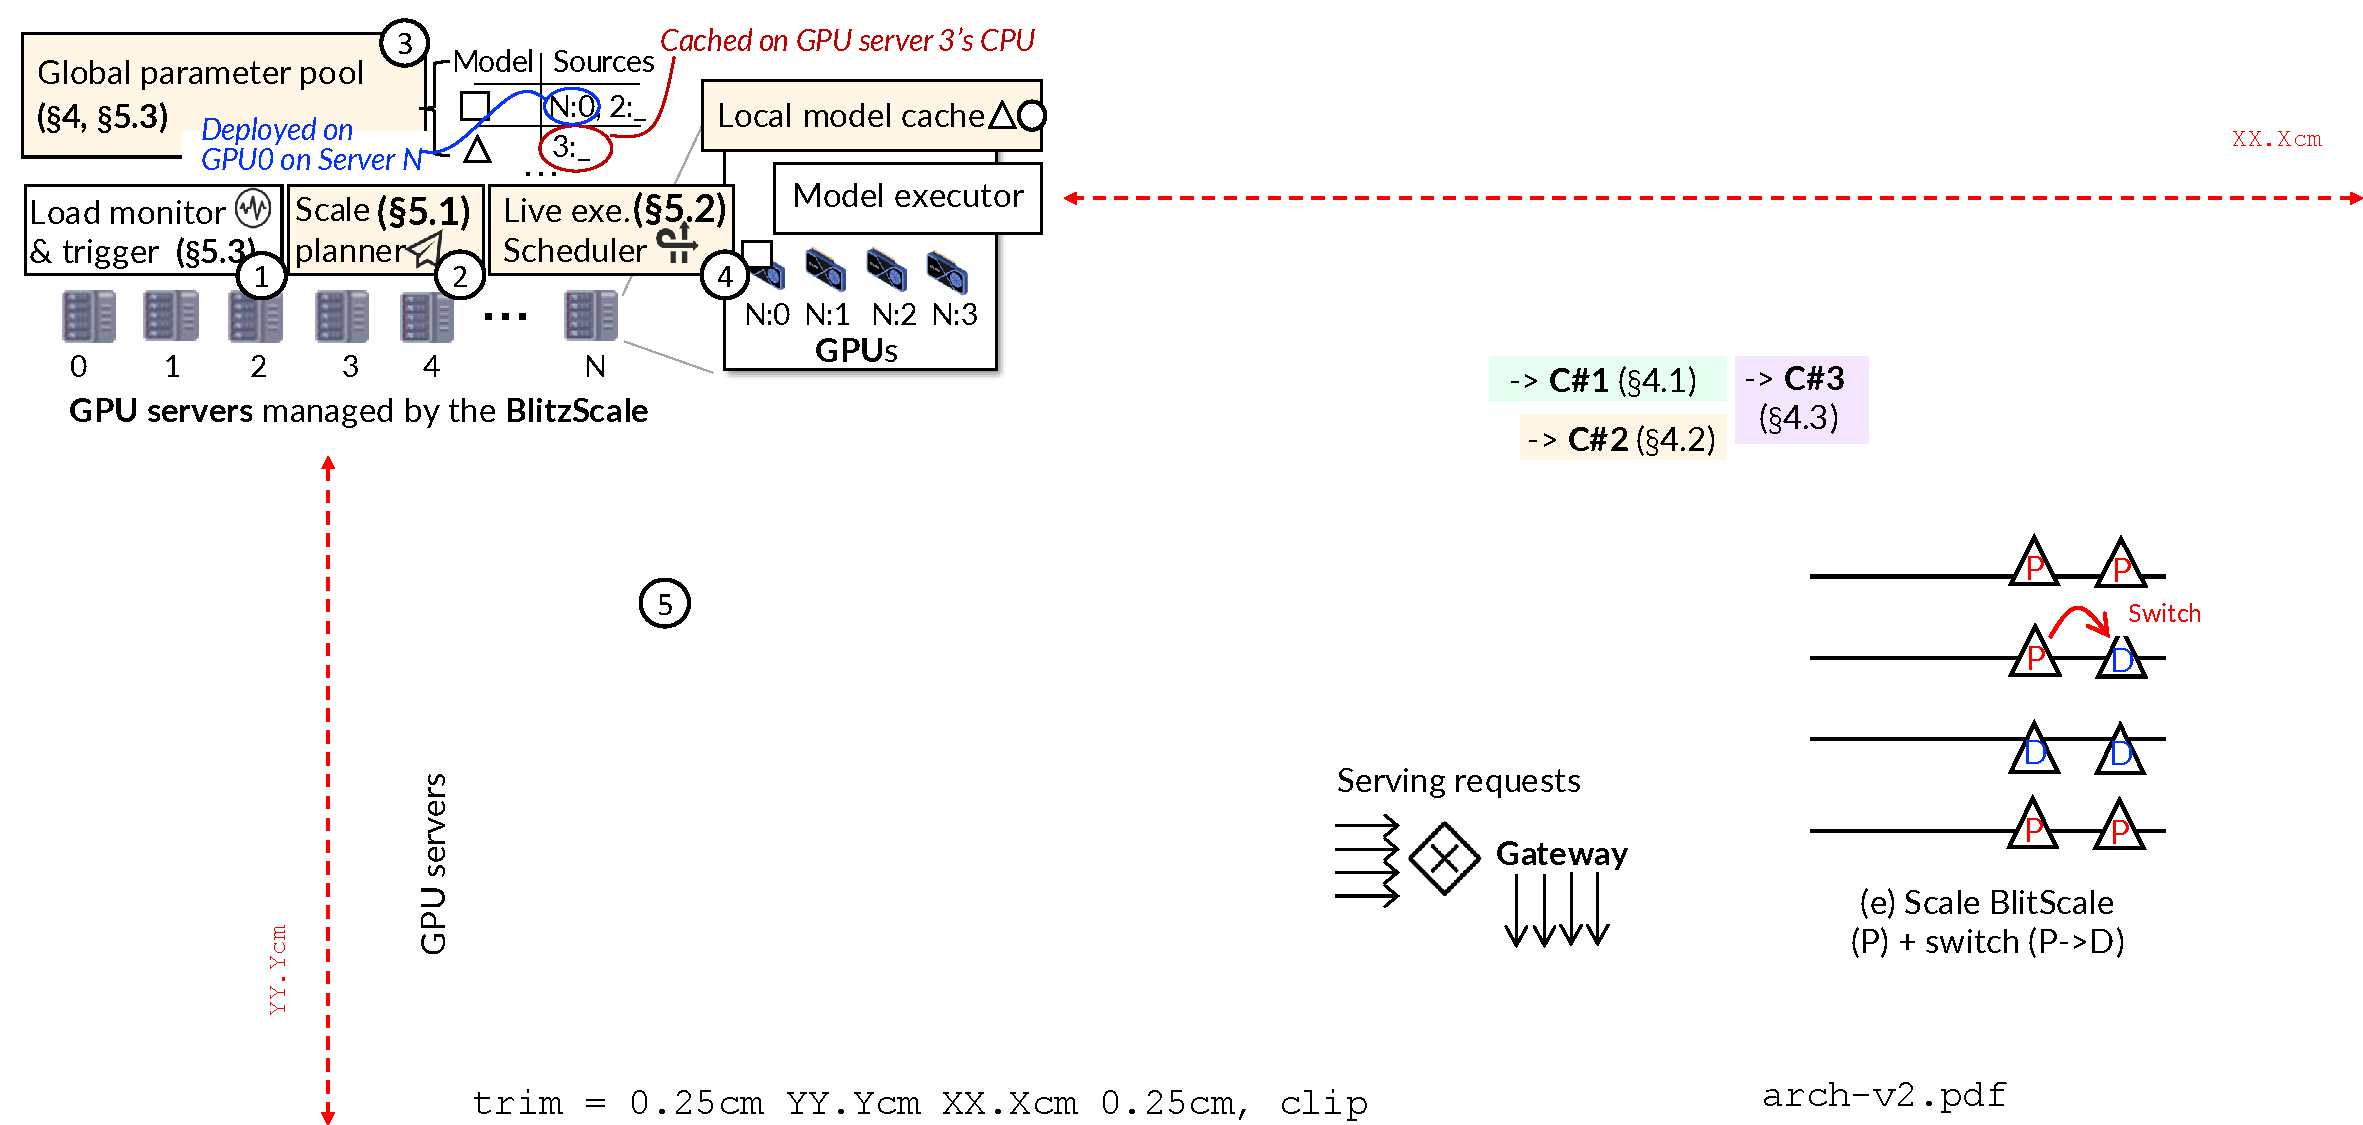
\includegraphics[width=.99\textwidth, trim=0.25cm 11.6cm 22.3cm 0.25cm, clip]{figs/arch-v2.pdf} \\[1pt]
    \end{minipage} \\[3pt]
    \begin{minipage}{1\linewidth}
        \caption{\small{\textit{
            {\sys} 的系统架构。
            由 {\sys} 新引入的模块用 {\fboxtwo} 标出。
        }}}
        \label{fig:arch}
    \end{minipage} \\[-10pt]
\end{figure}

\noindent
{\sys} 通过计算网络对模型进行扩缩，
即便主机缓存未命中，也能保持较快的扩缩速度。
为此，我们首先通过一个全局参数管理器来统一管理模型参数——
这些参数可能分散在服务实例背后的 GPU 上（针对已部署模型），
也可能位于主机 CPU 的缓存中。
该管理器维护模型与其参数来源之间的映射关系。
借助这一映射，
我们就能通过 RDMA 或 NVLink 这类高速互连，
迅速从相应来源读取参数。
除此之外，
我们还会把部分计算从过载实例卸载到那些仅完成部分参数加载的新实例上，
以实现在线扩缩容。

\stitle{系统架构与工作流程。\,}
{\fig{fig:arch}} 展示了系统架构。
与已有工作~\cite{DBLP:conf/usenix/Romero0YK21,DBLP:journals/corr/abs-2401-14351,DBLP:conf/osdi/SunHZXZL024} 类似，
我们有一个负载监控器（\ding{192}），
用于跟踪每个模型服务的负载情况，
并决定是否需要扩缩以及应扩出多少新实例（见 \textsection{\ref{sec:design-others}}）。
在每台机器上，
我们进一步采用现成的高性能 GPU kernel——FlashInfer~\cite{flashinfer}——来高效查询模型。
与现有系统相比，
{\sys} 的关键差异有两点。
第一，我们的扩缩规划器（\ding{193}）会结合全局参数管理器（\ding{194}）提供的信息，
生成一个扩缩计划，
用于指导如何通过计算网络高效地把参数加载到新扩出的实例上（见 \textsection{\ref{sec:design-plan}}）。
在图中的例子里，
新的实例既可以从主机 N 的 GPU0（记为 $(N,0)$）获取模型 {$\square$} 的参数，
也可以从主机 2 的 CPU 内存（记为 $(2,\_)$）获取。
第二，在扩缩期间，
我们的在线执行调度器（\ding{195}）会在实例之间重定向请求，
从而在参数尚未全部加载完成之前，就尽可能利用新实例的算力（见 \textsection{\ref{sec:design-pp}}）。

\begin{figure}[!t]
    \begin{minipage}{1\linewidth}
        \hspace{-1mm}
        \centering
        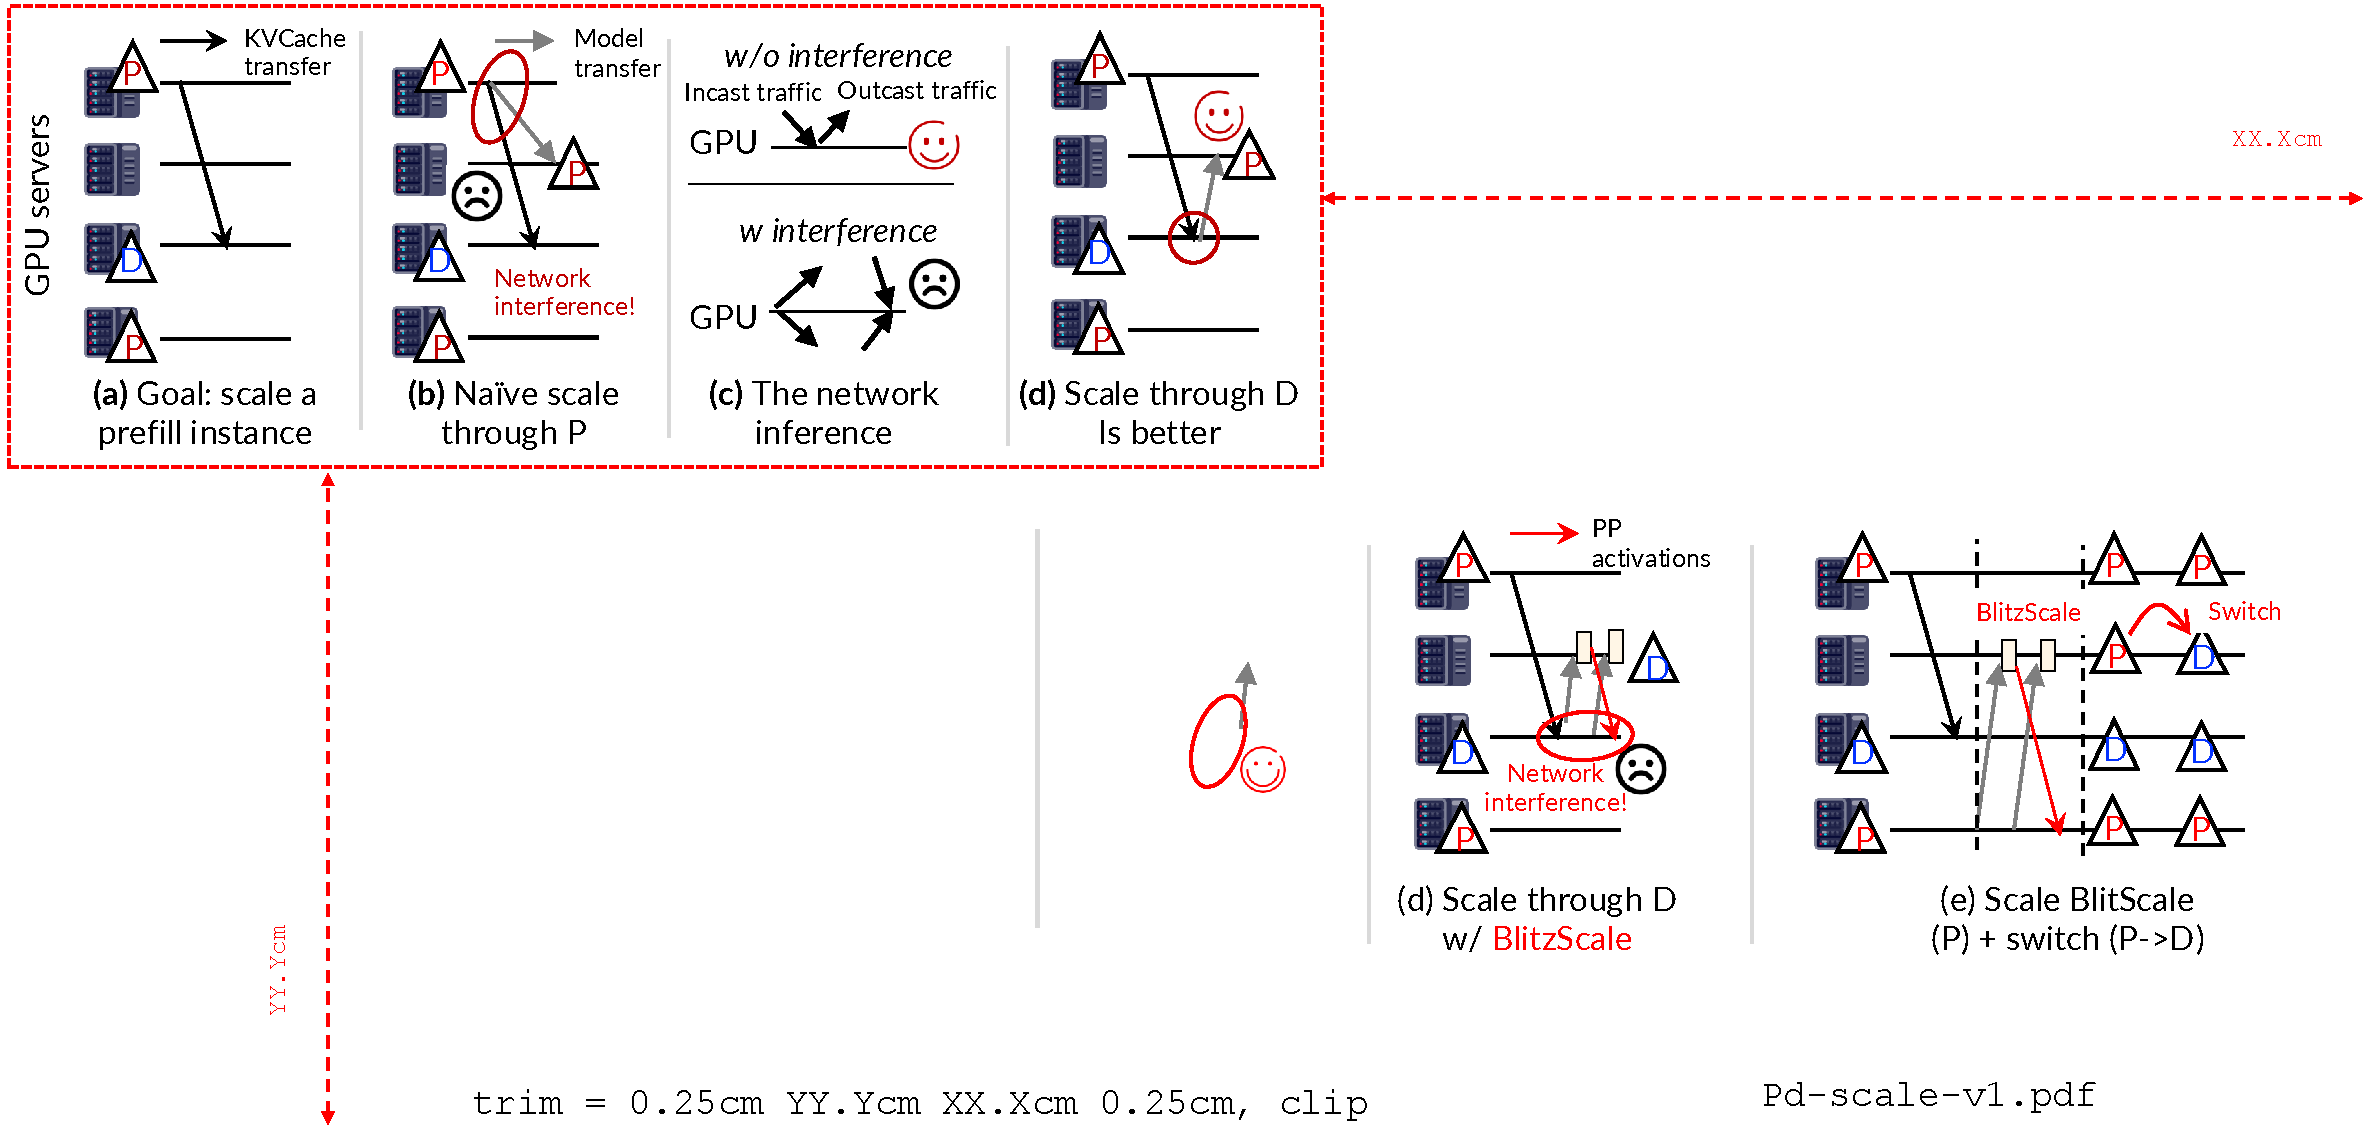
\includegraphics[width=.99\columnwidth, trim=0.25cm 11.3cm 17.7cm 0.25cm, clip]{figs/pd-scale-v1.pdf} \\[1pt]
    \end{minipage} \\[5pt]
    \begin{minipage}{1\linewidth}
        \caption{\small{\textit{
            (a) 在 LLM 的 Prefill/Decode 解耦服务中，扩一个 prefill 实例的示意图；
            (b) 如果直接从 prefill 实例扩缩，会引入网络干扰；
            (c) 利用现代数据中心网络的双向特性可以避免这种干扰；
            (d) 在考虑双向特性后得到的更优扩缩计划。
        }}}
        \label{fig:pd-scale}
    \end{minipage} \\[-10pt]
\end{figure}

\begin{figure}[!t]
    \centering
    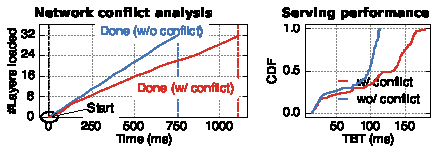
\includegraphics[left, scale=1.1]{./data/motiv-netconflict.pdf} \\[0pt]
    \begin{minipage}{1\linewidth}
        \caption{\small{\textit{
            网络干扰对 (a) 扩缩速度与 (b) 服务性能的影响分析。
        }}}
        \label{fig:motiv-network-conflict}
    \end{minipage} \\[-5pt]
\end{figure}

\stitle{挑战与方法。\,}
尽管我们利用了高速网络，
要让自动扩缩容同时具备“快速”和“在线”两种能力，
仍需解决以下挑战。

\emph{\textbf{挑战 1：在线生成无干扰的扩缩计划。} }
生成扩缩计划与生成\emph{多播}计划~\cite{DBLP:journals/jpdc/BhatRP03,DBLP:conf/asplos/CowanMMSX23,DBLP:conf/sc/GhazimirsaeedZR20,DBLP:conf/icpp/BanikazemiMP98,DBLP:conf/dsn/BehrensJBT18} 十分相似，
即如何把数据（这里是参数）从若干源快速分发到目标节点。
但自动扩缩容还有两项额外要求。
第一，计划必须能够在线生成，
因为源与目标会动态变化，
而在异构网络上求最优计划是 NP-hard 的~\cite{DBLP:journals/jpdc/BhatRP03}。
第二，计划必须消除参数加载与在线服务之间的网络干扰。
{\fig{fig:pd-scale}} 给出了采用 PD 解耦时的一个例子。
在这种设置下，
KVCache 会从 prefill 实例迁移到 decode 实例（见 (a)），
且这一迁移开销在正常情况下是可以被隐藏的~\cite{DBLP:conf/isca/PatelCZSGMB24}。
然而，如果我们想扩一个新的 prefill 实例，
并且像 (b) 那样直接把某个 prefill 实例选为参数源，
那么扩缩流量就会与 KVCache 迁移流量争夺网络带宽，
最终导致扩缩时间延长 1.5\,$\times$，
并使尾部 TBT 因 KVCache 迁移开销被放大而上升 50\,\%
（见 {\fig{fig:motiv-network-conflict}} (b)）。

针对这一问题，
我们基于三个观察设计了一个由服务负载指导的贪心计划生成方法（见 \textsection{\ref{sec:design-plan}}）。
第一，网络异构性的主要来源是 NVLink，
而 NVLink 的速度极高：
例如它能在 120\,ms 内把一个 Llama3-8B 广播到 8 张 GPU 上。
因此，我们可以把通过 NVLink 相连的实例抽象成一个逻辑实例组，
从而在规划时把 NVLink 从网络拓扑中消去。
第二，通过网络加载参数是一个带宽密集型过程，
因此我们可以用串行转发链~\cite{DBLP:conf/icpp/VerstoepLB96} 的方式贪心构造多播，
这在常见场景下是最优的。
第三，GPU 服务器之间的 RDMA 网络通常具备双向特性~\cite{288657,rdma-bidirectional}，
也就是说，入向（incast）与出向（outcast）流量不会相互干扰（见 (c)）。
因此，我们可以在计划生成时移除那些会在同一链路、同一方向上产生冲突的流，
从而规避干扰。
例如，我们可以像 {\fig{fig:pd-scale}} (d) 那样，
从 decode 实例向 prefill 实例加载参数。

\begin{figure*}[!t]
    \begin{minipage}{1\linewidth}
        \hspace{-1mm}
        \centering
        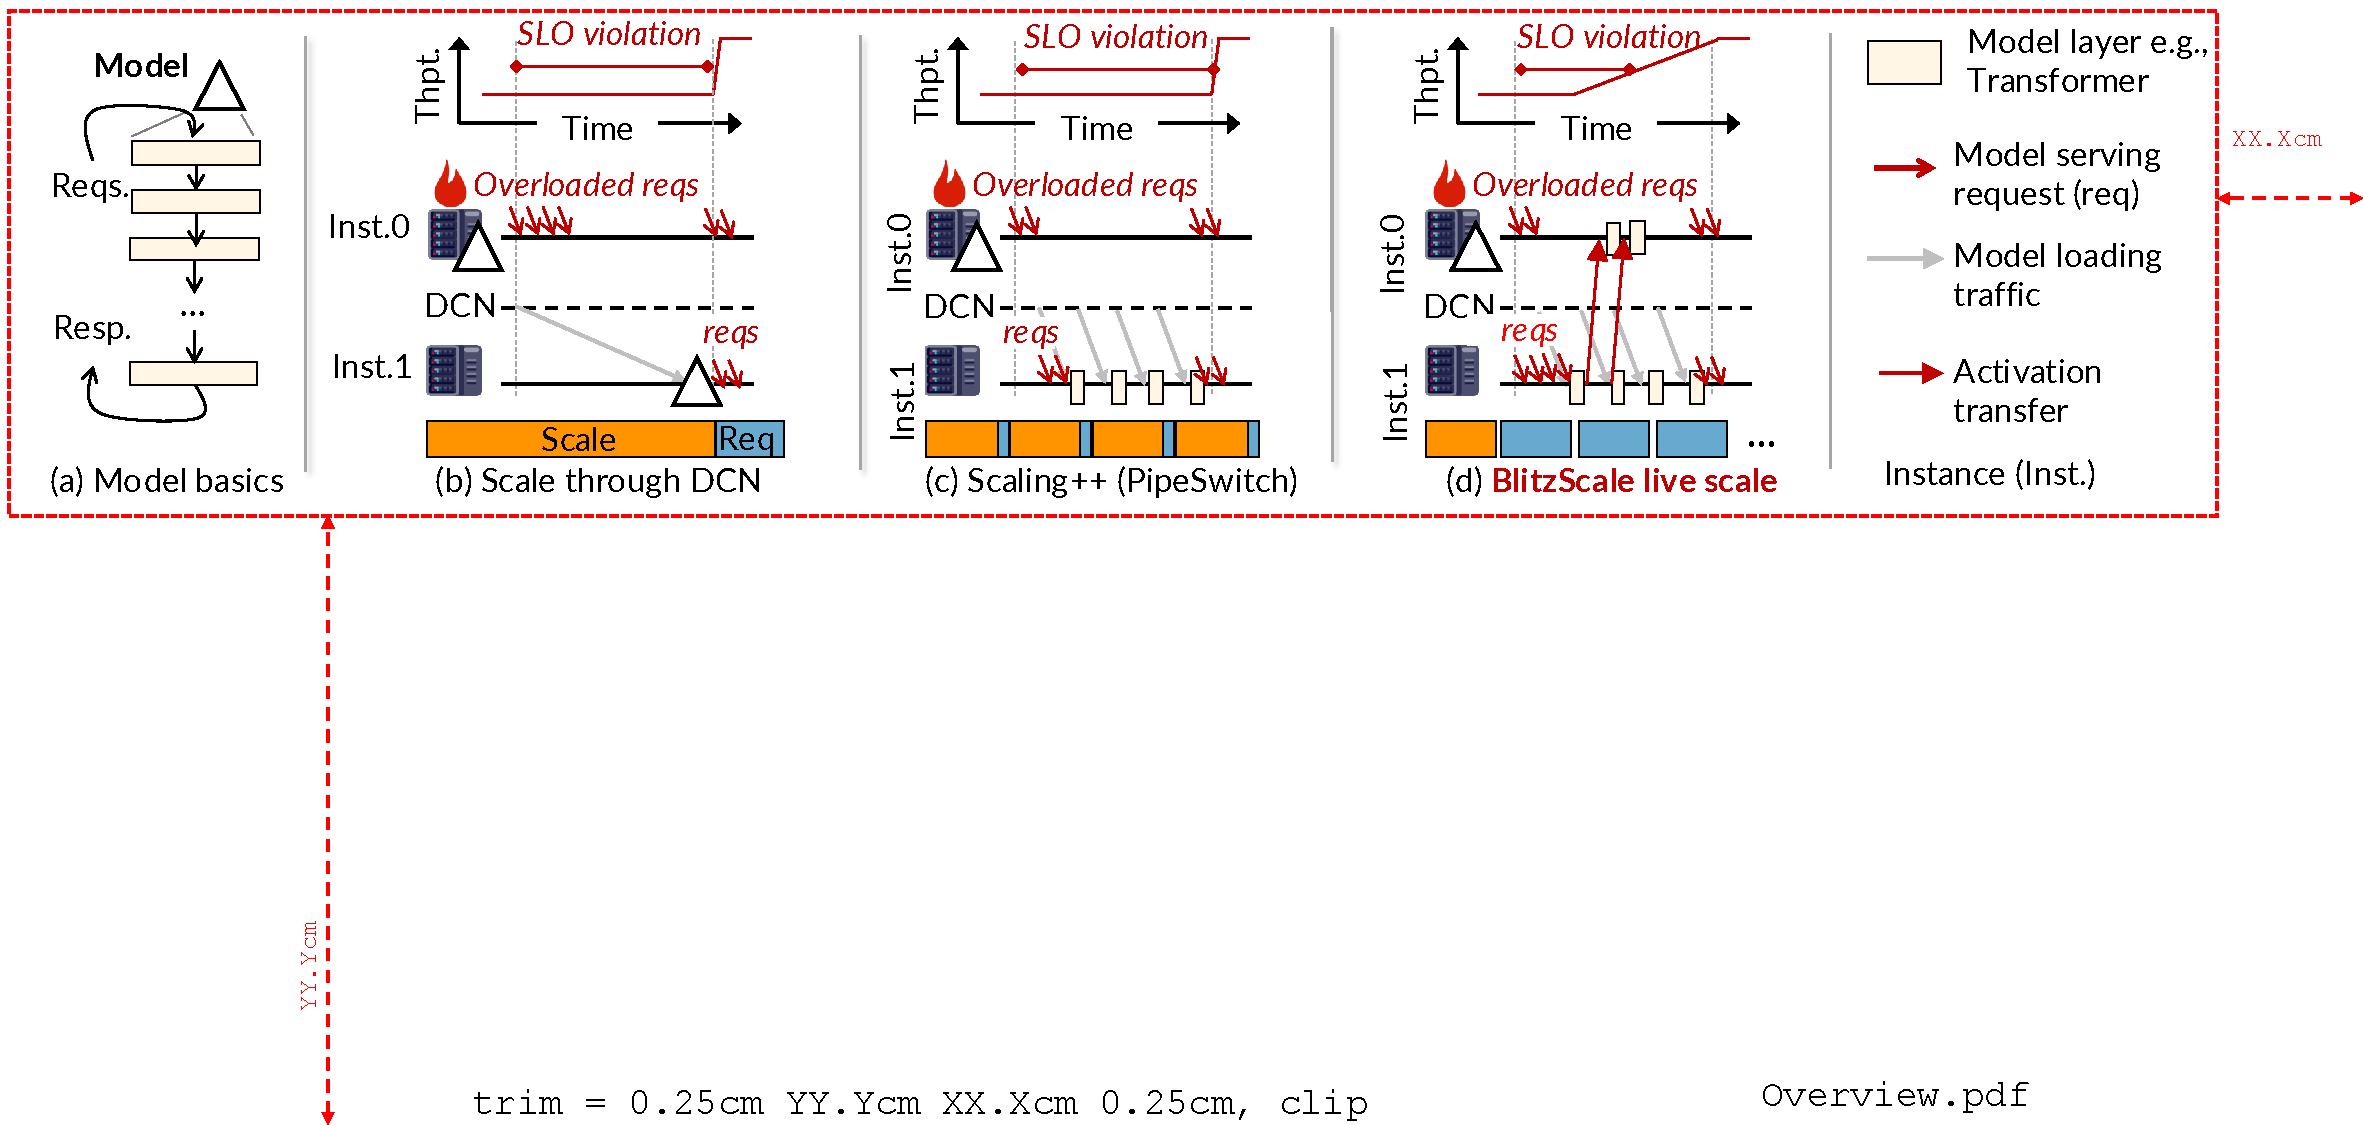
\includegraphics[width=.95\columnwidth, trim=0.25cm 10.38cm 2.5cm 0.25cm, clip]{figs/overview.pdf}
    \end{minipage} \\[8pt]
    \begin{minipage}{1\linewidth}
        \caption{\small{\textit{
            (a) 模型执行请求的整体过程；
            (b) 通过数据中心网络（DCN）进行朴素模型扩缩的示意；
            (c) 一种与执行重叠的改进扩缩方式~\cite{pipeswitch}，但它仍然不是在线的；
            (d) {\sys} 如何实现在线扩缩。
        }}}
        \label{fig:overview}
    \end{minipage} \\[-10pt]
\end{figure*}

\vspace{1.ex}
\emph{\textbf{挑战 2：实现在线自动扩缩容。} }
在线自动扩缩容——即在所有参数尚未加载完成之前，新实例就能提升系统吞吐——之所以必要，
是因为即便使用了高速网络，
仍然可能出现 SLO 违约（见 {\fig{fig:motiv-scale-speed}} (c)）。
而现有系统很难做到这一点。
例如，PipeSwitch~\cite{pipeswitch} 与 DeepPlan~\cite{deepplan}
都利用模型逐层执行的特性来进行推理。
如 {\fig{fig:overview}} (c) 所示，
一旦 inst.1 上的第一层加载完成，
它们就会把过载请求重定向给 inst.1 执行；
同时，inst.1 会并行加载后续层。
但这样的重叠并不是真正的在线扩缩，
因为在所有层都加载完成之前，
inst.1 依然无法独立完成一个请求，
也就无法真正提升系统整体吞吐。

为此，
我们提出了一种新的协同执行方案来实现在线自动扩缩容。
核心观察在于：
虽然新扩出的实例在所有层加载完之前无法独立完成请求，
但它可以利用已经加载好的层去分担过载实例上的部分计算，
从而提升整体服务吞吐。
{\fig{fig:overview}} (d) 展示了这一思想。
当 inst.0 过载、而 inst.1 正在扩缩时，
在 inst.1 加载完第一层之后，
我们会把所有请求从 inst.0 重定向到 inst.1 执行第一层。
当 inst.1 完成第一层计算后，
它再把 activation 发回 inst.0，
由 inst.0 执行剩余层。
这样一来，
系统吞吐会上升，排队时延随之下降。
要理解吞吐为何增加，
可以考虑一个 7 层模型：
若只有 inst.0 单独服务，其吞吐为 1/7；
在我们的在线扩缩方式下，
一旦 inst.1 加载好 1 层，inst.0 只需执行剩下 6 层，
其等效吞吐就提升到 1/6。
随着 inst.1 加载的层数继续增加，
吞吐还会进一步提高；
当一半层加载完成时——也就是扩缩时间过去一半时——系统吞吐达到峰值（翻倍）。
\textsection{\ref{sec:design-pp}} 将进一步介绍我们用于协调过载实例与新实例的 ZigZag 调度方法，
以在在线扩缩过程中获得最佳性能。

\section{详细设计与实现}
\label{sec:design}

\subsection{在线网络化扩缩计划生成}
\label{sec:design-plan}

\noindent
当规划器收到“把参数扩到 $n$ 张新 GPU 上”的通知后，
它会从参数池中获取 $s$ 个参数源，
选择 $t$ 个空闲 GPU 作为目标，
并生成一个计划，决定如何把参数从这 $s$ 个源发送到这 $t$ 个目标中的某些 GPU 上。
在计划生成时，我们希望同时最小化三项指标：
(1) 扩缩时间；
(2) 计划生成时间；
(3) 与在线服务工作负载之间的干扰。

\begin{figure}[!t]
    \begin{minipage}{1\linewidth}
        \hspace{-1mm}
        \centering
        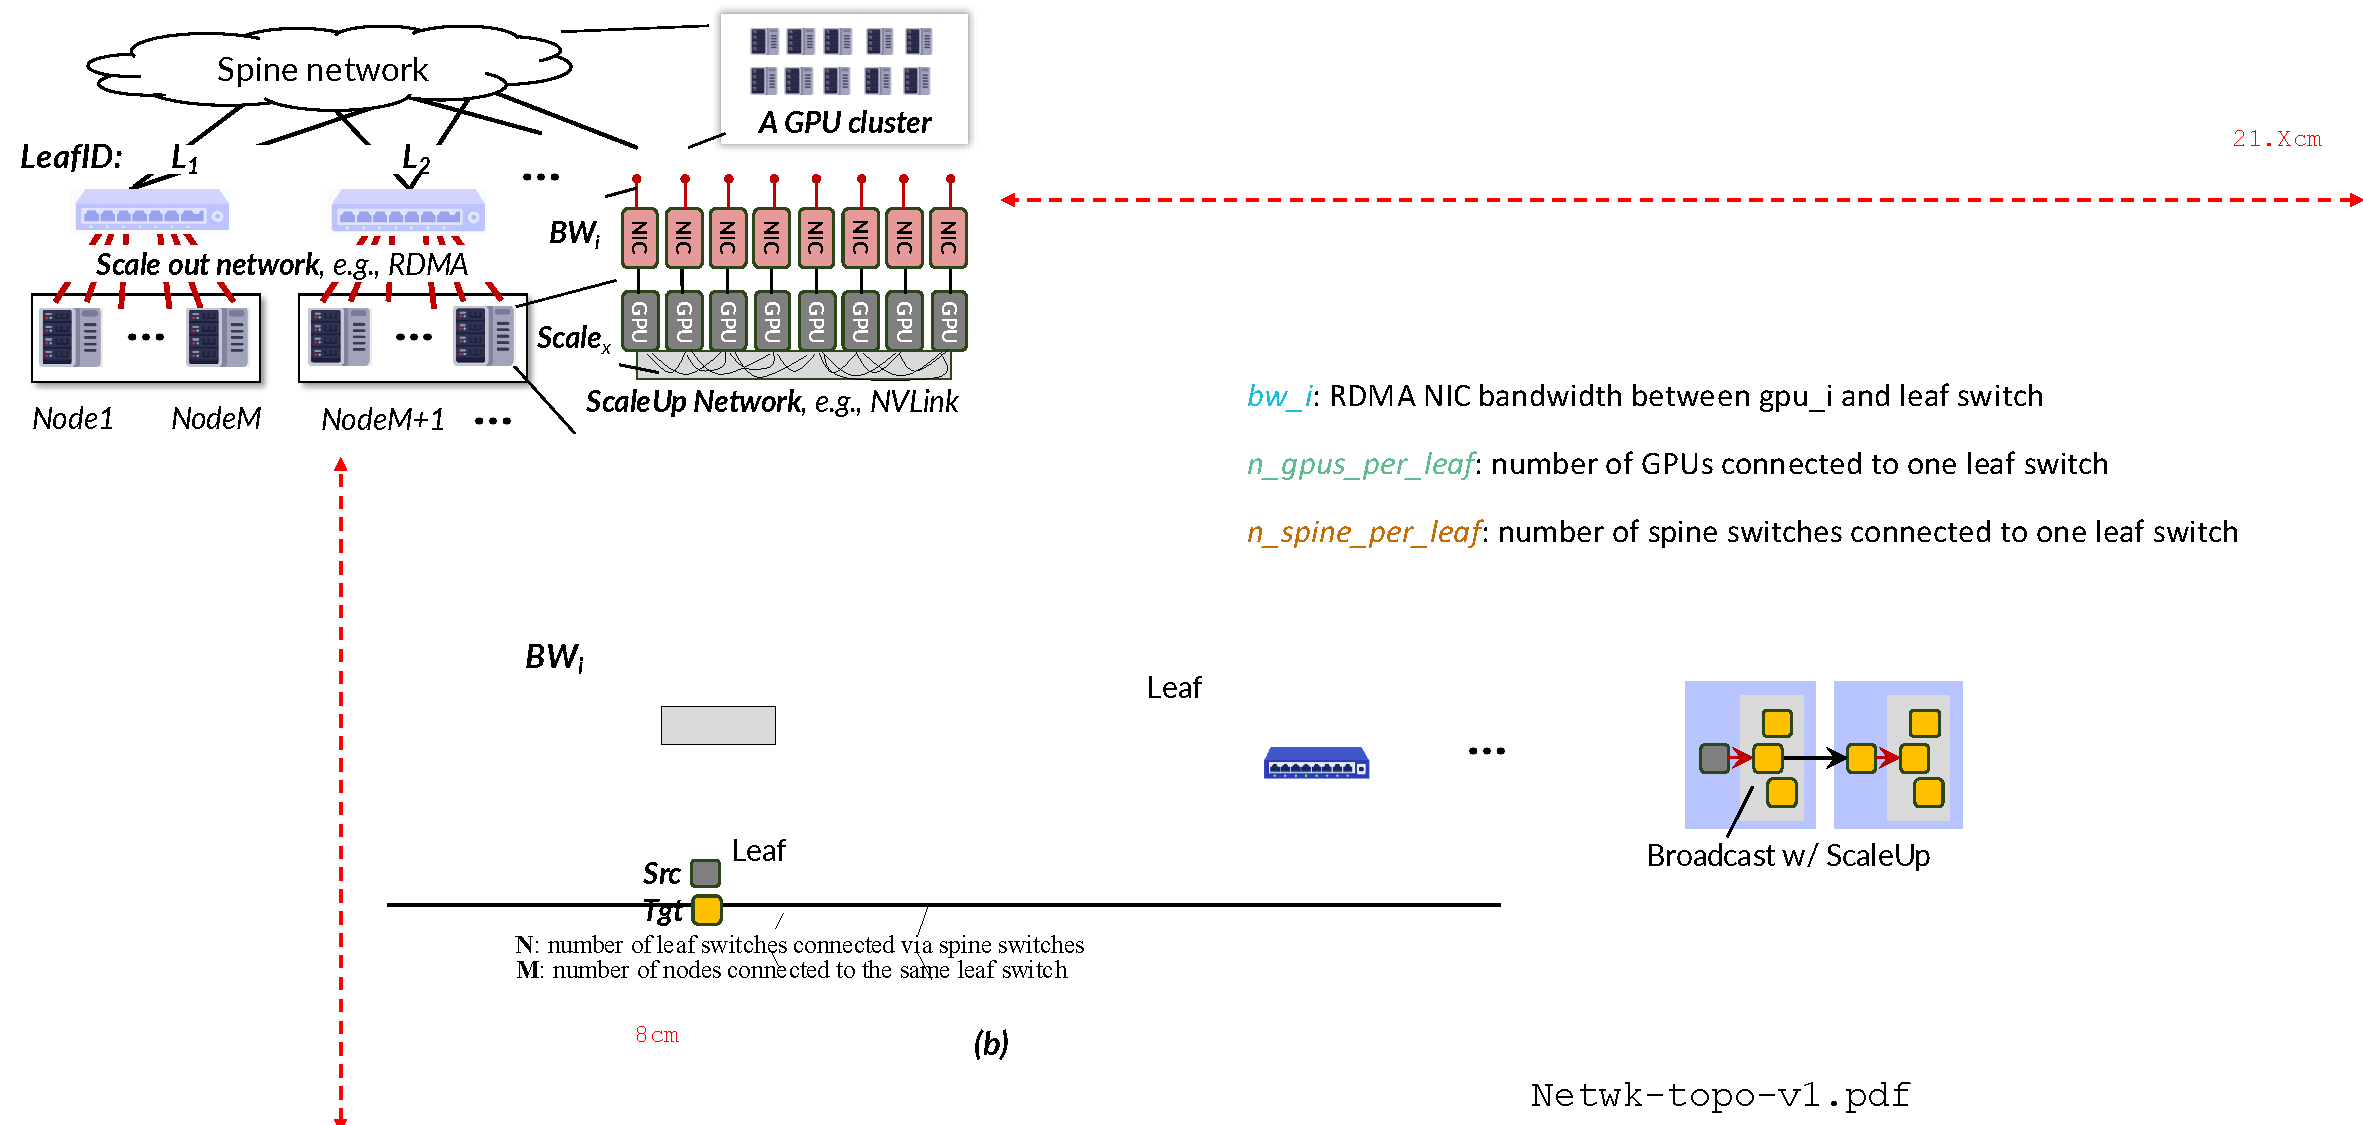
\includegraphics[width=1\textwidth, trim=0.25cm 11.45cm 23.1cm 0.25cm, clip]{figs/netwk-topo-v1.pdf}
    \end{minipage} \\[2pt]
    \begin{minipage}{1\linewidth}
        \caption{\small{\emph{
            {\sys} 如何对网络建模的示意图。
        }}}
        \label{fig:network-topo}
    \end{minipage} \\[-20pt]
\end{figure}

\stitle{GPU 间网络建模。\,}
要高效生成扩缩计划，
首先需要对参数源与目标之间的网络进行建模。
但在服务集群中，网络拓扑往往非常复杂，
这项工作并不简单。
我们的模型假设集群采用一种简化的 scale-up 与 scale-out 混合网络结构，
而这正是现代 GPU 集群中广泛采用的方式~\cite{dellAiFabric, DBLP:conf/hoti/WangGSZH24, nvidia-compute-network}。
{\fig{fig:network-topo}} (a) 展示了这一建模方法。

首先，
我们把通过 NVLink 这类高速 scale-up 网络相连的 GPU 建模为一个 GPU 组。
这些 GPU 之间具有极高的互连带宽（1,600--3,600\,Gbps），
因此在组内完成扩缩的开销可以忽略不计。
相比之下，
通过 RDMA 这类较慢 scale-out 网络相连的 GPU 更难建模，
因为其拓扑通常呈现层次结构。
为此，
我们采用一个简单的 leaf-to-spine 模型，
它能够覆盖包括 Clos 与 Rail-optimized 在内的多种广泛部署拓扑~\cite{DBLP:conf/hoti/WangGSZH24}，
并支持不同的订阅比。
在该模型中，
每张 GPU（$i$）都以带宽 $BW_i$ 连接到一个叶子交换机（\text{LeafID}）；
同一叶子交换机下的 GPU 之间形成全互连，
也就是说，GPU $i$ 与 GPU $j$ 之间的带宽为 $\min(BW_i, BW_j)$。
更高一层，叶子交换机连接到 spine 交换机，
其叶间带宽小于或等于叶内带宽。
为简化起见，
我们不显式建模 spine 层，
而是假设上层协议（例如 Virtual Link Trunking, VLT~\cite{DellVLTPatent2016} 以及 Equal-Cost Multi-Path, ECMP~\cite{RFC2992}）
足以支持高效的叶间网络通信。

\begin{figure}[!t]
    \begin{minipage}{1\linewidth}
        \hspace{-1mm}
        \centering
        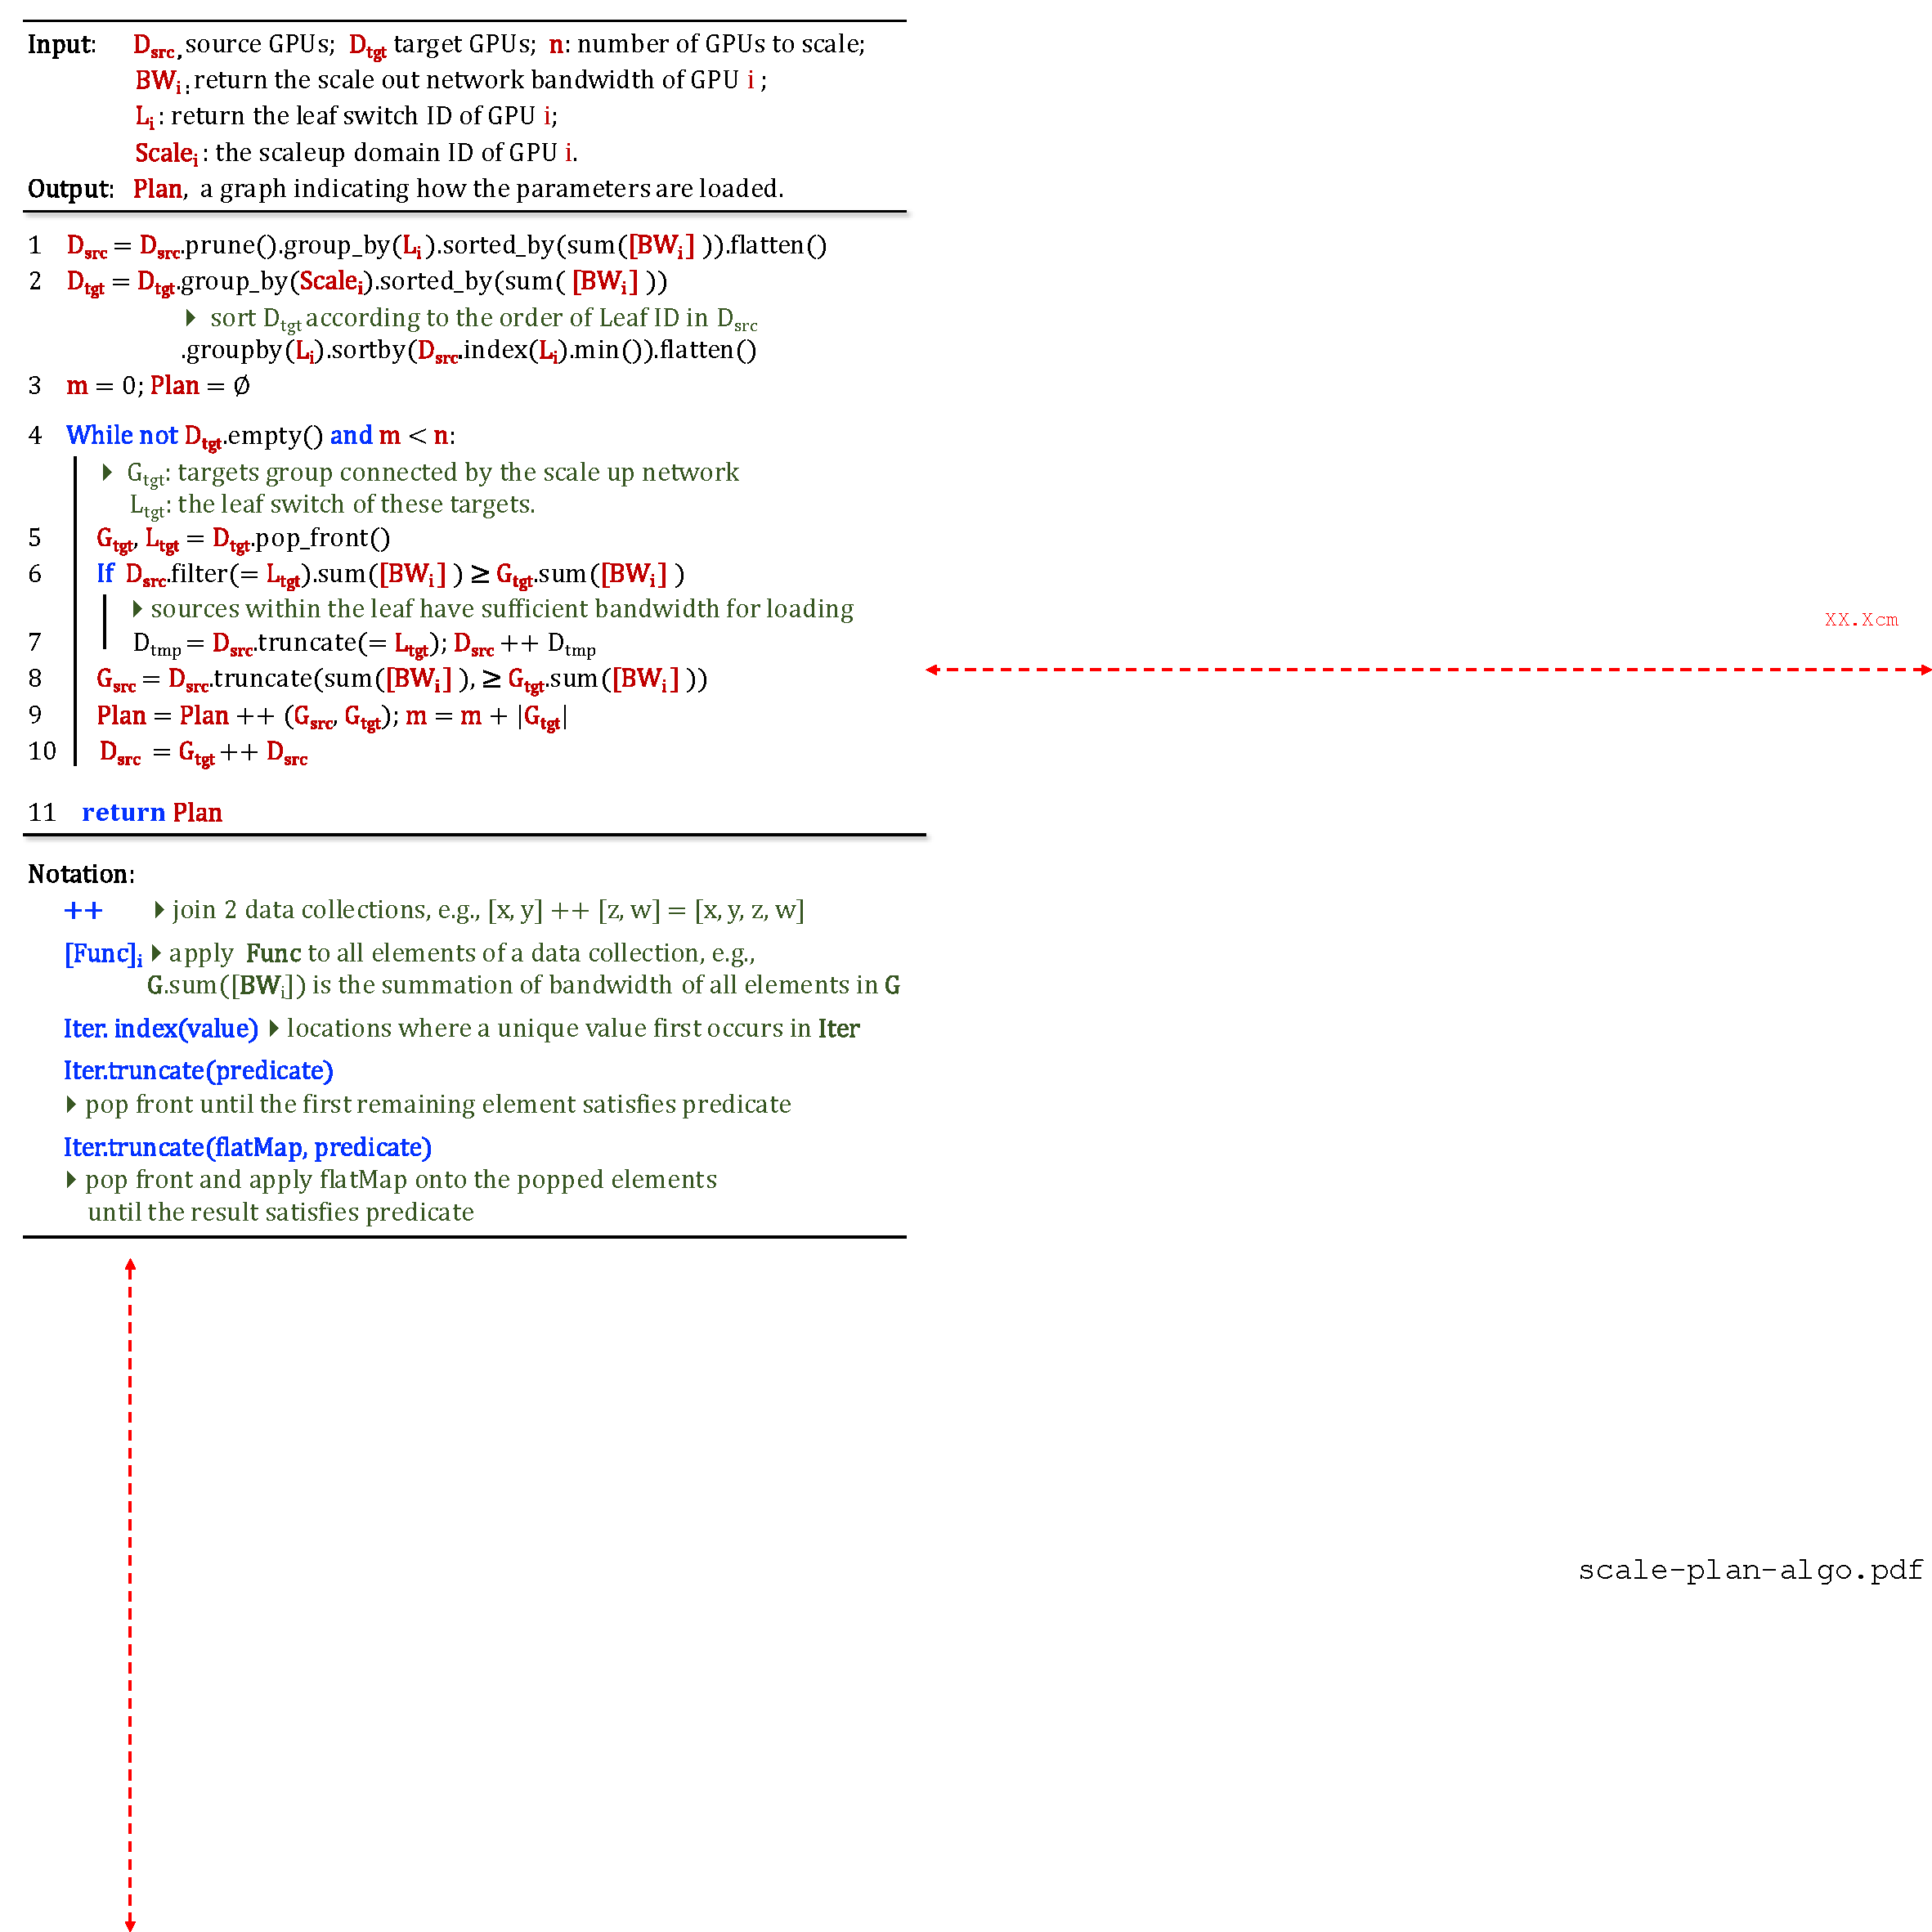
\includegraphics[width=1\textwidth, trim=0.25cm 14cm 21cm 0.25cm, clip]{figs/scale-plan-algo.pdf} \\[1pt]
    \end{minipage} \\[3pt]
    \begin{minipage}{1\linewidth}
        \caption{\small{\textit{
            计划生成算法的伪代码。
        }}}
        \label{alg:alg-plan}
    \end{minipage} \\[-15pt]
\end{figure}

\stitle{基于多播链的贪心计划生成。\,}
为了能够在线快速生成计划，
我们采用如算法~\ref{alg:alg-plan} 所示的三步贪心算法。
第一步，
通过剪枝参数源，避免其与在线服务工作负载发生任何干扰（第 1 行）。
第二步，
把通过 NVLink 等 scale-up 网络连接的目标节点聚合成组（第 2 行），
从而可以利用 NVLink 广播高效完成并行的切分参数传输（见 {\fig{fig:parallel-shards}}）。
最后，
我们构造多条串行广播链（第 3--10 行）来形成最终扩缩计划。

\begin{figure}[!t]
    \begin{minipage}{1\linewidth}
        \hspace{-1mm}
        \centering
        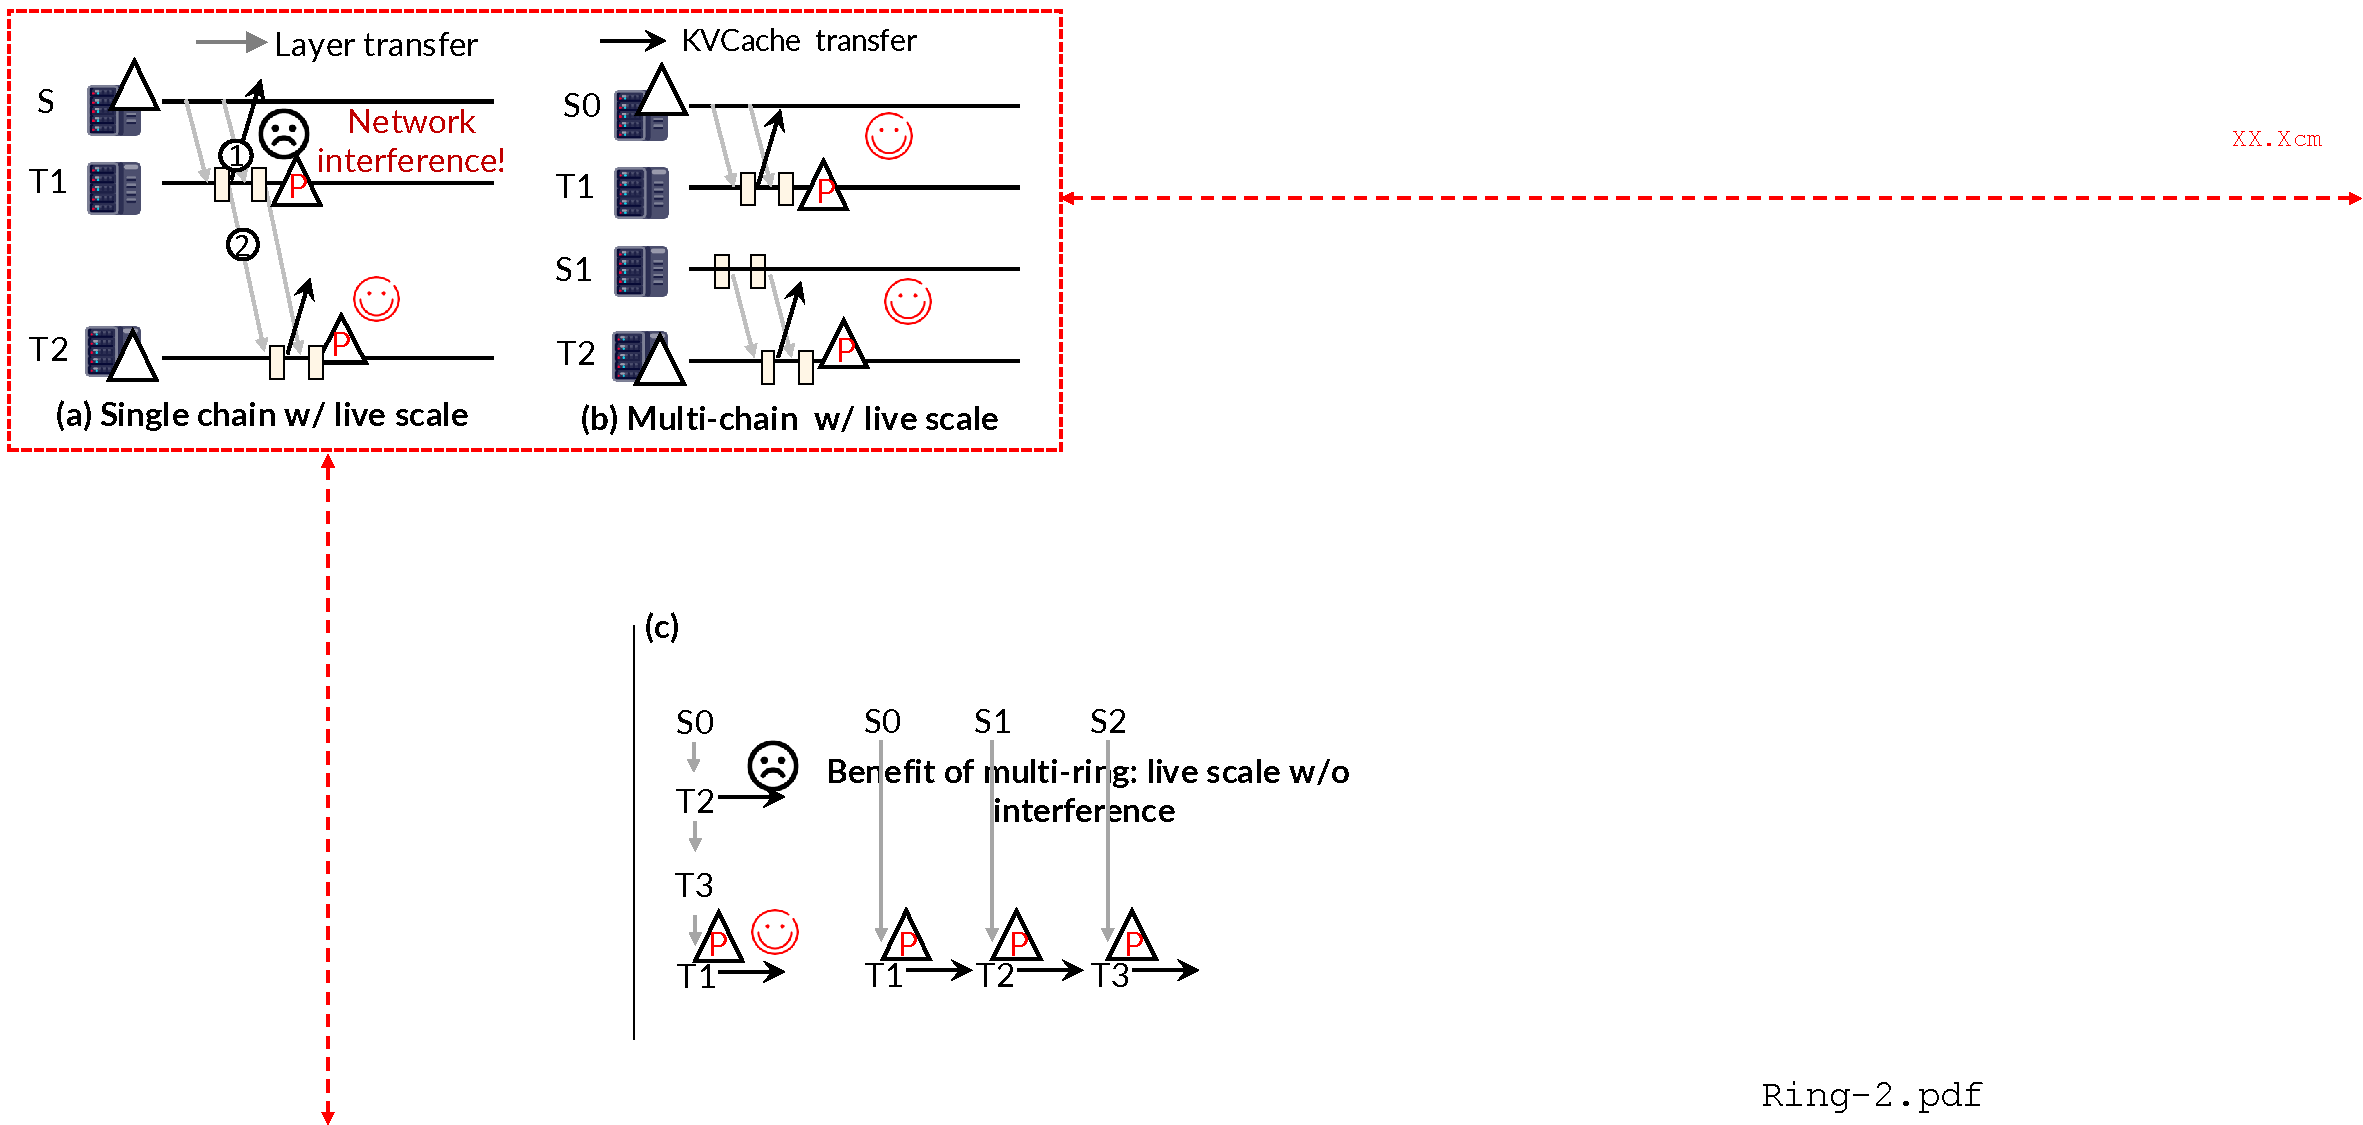
\includegraphics[width=1\textwidth, trim=0.25cm 11.6cm 23cm 0.25cm, clip]{figs/ring-2.pdf} \\[1pt]
    \end{minipage} \\[4pt]
    \begin{minipage}{1\linewidth}
        \caption{\small{\emph{
            为什么多条广播链更好，尤其是在在线扩缩场景中。
        }}}
        \label{fig:ring-2}
    \end{minipage} \\[-15pt]
\end{figure}

\begin{figure}[!t]
    \begin{minipage}{1\linewidth}
        \hspace{-1mm}
        \centering
        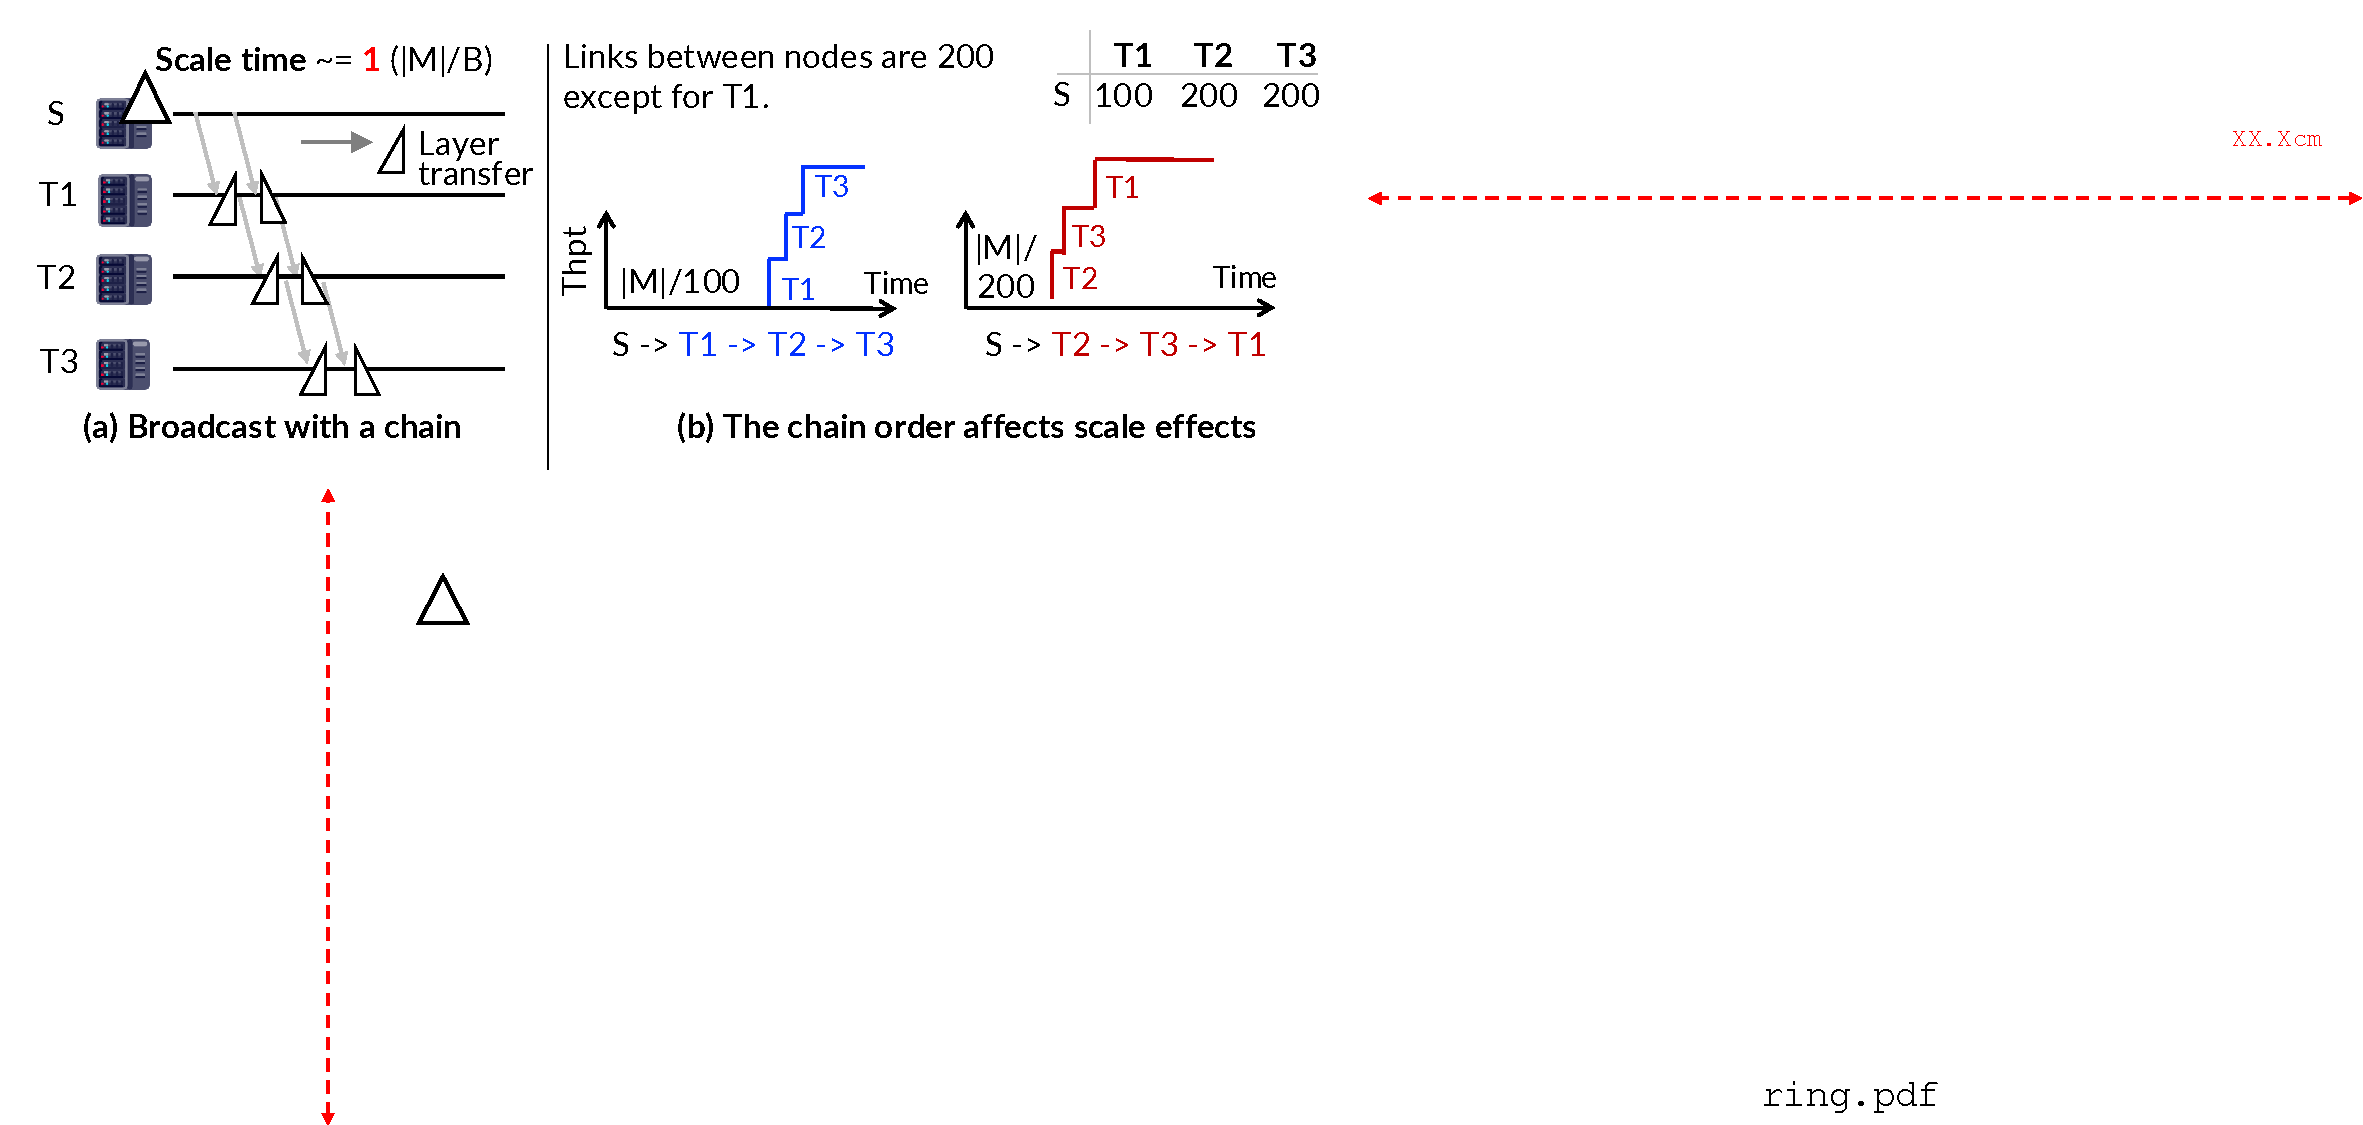
\includegraphics[width=1\textwidth, trim=0.25cm 11.6cm 17.5cm 0.25cm, clip]{figs/ring.pdf}
    \end{minipage} \\[7pt]
    \begin{minipage}{1\linewidth}
        \caption{\small{\emph{
            (a) 为什么广播链适合高带宽需求的大规模传输；
            (b) 为什么我们选择特定的链顺序。
            $|M|$ 表示模型大小，$B$ 表示一条链中最慢链路的带宽。
        }}}
        \label{fig:ring}
    \end{minipage} \\[-10pt]
\end{figure}

具体来说，
一条串行广播链由若干源节点与目标节点组成，
形式为 $S \rightarrow T_1 \rightarrow T_2 \rightarrow ... \rightarrow T_n$。
需要注意的是，一条链中的每个节点都可能包含多张 GPU。
这种链式结构有一个非常好的性质：
对于模型扩缩这种带宽密集型传输场景，
其整体传输时间几乎与接收实例数量无关，因此是最优的。
如 {\fig{fig:ring}} (a) 所示，
当 $T_1$ 收到第一层参数后，
它会立刻把该层转发给 $T_2$；
与此同时，源节点 $S$ 则继续把第二层发送给 $T_1$，
于是第一层与第二层的发送时间能够彼此重叠。

对于带宽均匀的网络，
单条串行链通常已足够高效。
但在叶脊网络中，叶间带宽往往存在差异，
而且在我们的在线扩缩场景里，
多条链是必要的。
原因有两点：
(1) 当每个叶子交换机下同时存在源和目标时，多条链可以避免较慢的叶间通信（第 6--7 行）；
(2) 在 PD 解耦场景中，多条链还能够创造更多无干扰的在线扩缩机会。
{\fig{fig:ring-2}} 展示了后一种情况：
假设我们想在线扩出两个 prefill 实例，
那么在 prefill 完成后，KVCache 需要被传到 decode 实例。
如果只使用一条链，
那么只有 $T_2$ 可以在不产生网络干扰的情况下参与在线扩缩，
因为在 $T_1$ 处，KVCache 传输（\ding{192}）会与参数转发流量（\ding{193}）发生冲突。
若改用两条链，并由两个参数源分别支撑（图 (b)），
那么 $T_1$ 与 $T_2$ 都可以在无干扰的条件下参与在线扩缩。

需要注意的是，
链中节点的顺序同样非常重要。
我们按照节点之间聚合链路带宽的降序来排列节点（第 2 行、第 5 行）。
这样做的原因是，
优先向高带宽节点发送参数，
能够更快地提升整体服务吞吐。
如 {\fig{fig:ring}} (b) 所示，
假设源节点 $S$ 向 $T_2$ 发送参数的速度是向 $T_1$ 的两倍，
那么链顺序 $S \rightarrow T_2 \rightarrow T_1$ 就优于 $S \rightarrow T_1 \rightarrow T_2$，
因为前者中 $T_2$ 的停机时间只有后者的一半。
此外，在我们的设置中，
源节点本身也可以是一个 GPU 组，
因为 GPU 往往配有独立网卡。

\begin{figure}[!t]
    \begin{minipage}{1\linewidth}
        \hspace{-1mm}
        \centering
        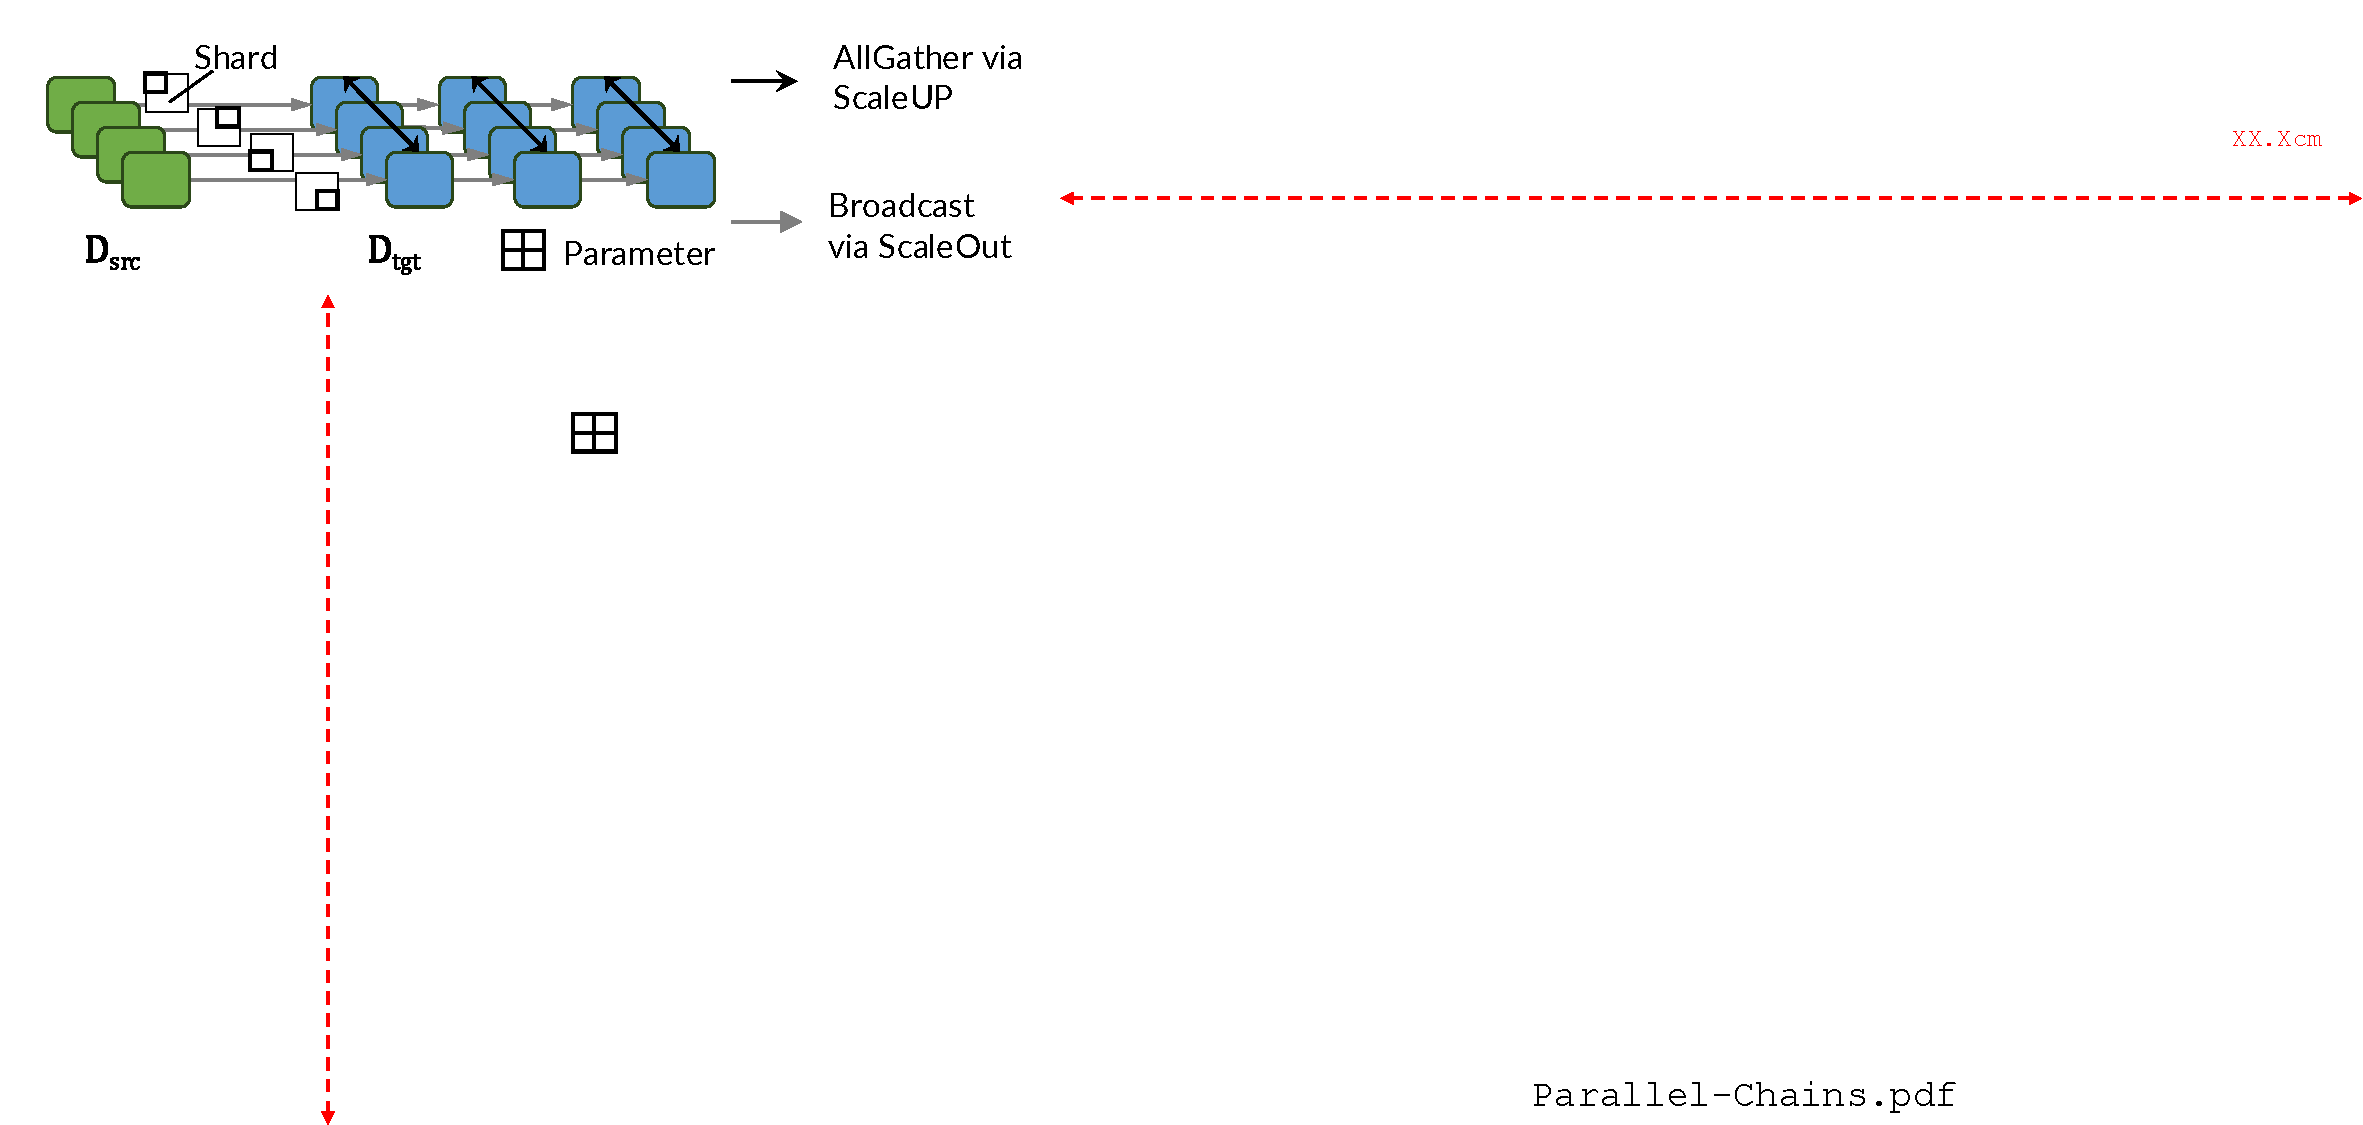
\includegraphics[width=1\textwidth, trim=0.25cm 14.2cm 22.5cm 0.25cm, clip]{figs/parallel-shards.pdf} \\[1pt]
    \end{minipage} \\[4pt]
    \begin{minipage}{1\linewidth}
        \caption{\small{\emph{
            利用 scale-up 网络进行切分参数并行传输的示意图。
        }}}
        \label{fig:parallel-shards}
    \end{minipage} \\[-15pt]
\end{figure}

\stitle{优化：来自多源的并行切分参数传输。\,}
\label{sec:design-shard}
对于一条广播链，
如果其源节点与目标节点内部都包含拥有重复参数的多张 GPU，
那么我们还可以进一步利用 scale-up 网络对链路传输进行并行化。
{\fig{fig:parallel-shards}} 给出了一个具体例子。
假设源节点与目标节点各有 4 张 GPU。
在这种情况下，
每张源 GPU 只需要向对应的目标 GPU 转发 1/4 的切分参数；
随后目标侧 GPU 再通过基于 NVLink 的 AllGather 获得完整参数。
由于 NVLink AllGather 的时间可以忽略，
这种方式能够把扩缩时间缩短到原来的 1/4。

\subsection{利用 ZigZag 调度实现高效在线扩缩容}
\label{sec:design-pp}

\nospacestitle{为在线扩缩选择实例。\,}
在通过算法~\ref{alg:alg-plan} 得到若干广播链之后，
我们会根据以下两个条件选择哪些实例参与在线扩缩：
(1) 在线扩缩是否有必要，也就是 stop-the-world 扩缩是否会导致 SLO 违约；
(2) 是否存在能够与之协同执行的过载实例。
这两个条件都很容易获得：
第一，我们可以利用 {\fig{fig:motiv-scale-speed}} 中“加载速度—SLO 违约率”之间的对应关系进行判断；
第二，自动扩缩一般只会在系统过载时触发。
因此，对每个过载实例，
我们都会在广播链中识别一个满足条件 (1) 的新实例，
通常是链尾实例，因为它们所处链路最慢，更有可能需要在线扩缩。

\stitle{成对实例上的在线扩缩协议。\,}
假设我们已经选定一个新实例（inst.1），
用于从一个过载实例（inst.0）上卸载部分计算。
为了启动在线扩缩，
我们采用一个三阶段的状态转换协议：
(1) 一旦 inst.1 开始加载参数，
我们就把 inst.0 上所有排队请求以及新到请求全部重定向到 inst.1。
由于请求负载远小于模型参数，
这一步的重定向开销可以忽略不计。
(2) 当第一层参数加载到 inst.1 后，
它便开始执行所有请求的第一层。
需要注意的是，在第一层加载期间，
inst.0 仍继续处理自己当前的待执行请求。
最后，
当 inst.1 完成全部模型参数加载后（阶段 (3)），
请求就会重新在两个实例之间平均分配。

\begin{figure}[!t]
    \begin{minipage}{1\linewidth}
        \hspace{-1mm}
        \centering
        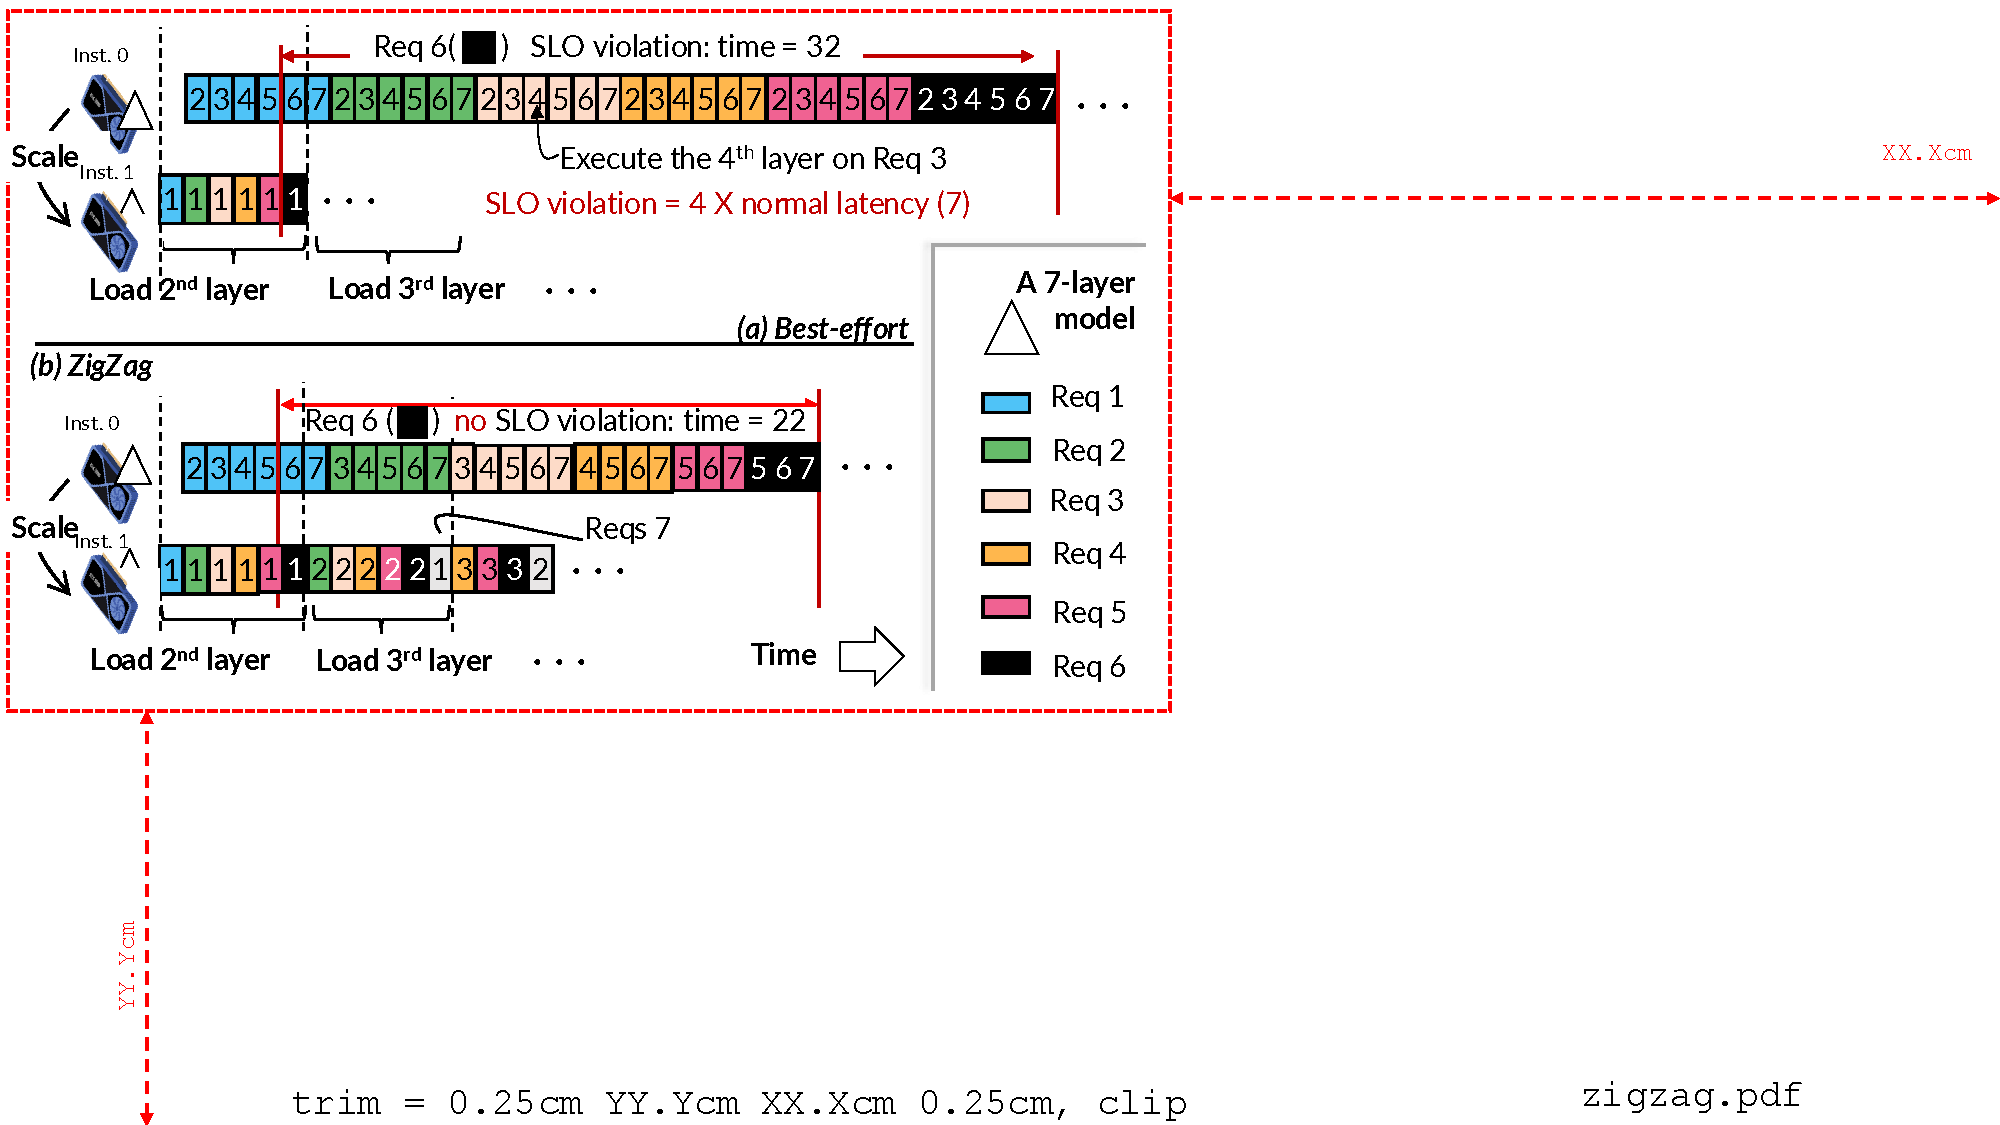
\includegraphics[width=1\textwidth, trim=0.25cm 7.1cm 14.2cm 0.25cm, clip]{figs/zigzag.pdf} \\[1pt]
    \end{minipage} \\[3pt]
    \begin{minipage}{1\linewidth}
        \caption{\small{\textit{
            ZigZag 调度必要性的示意图。
            注意，执行从第 1 层被加载到实例 1（inst.1）后开始。
            这里假设加载 1 层所需时间可以完成 6 层计算。
        }}}
        \label{fig:zigzag}
    \end{minipage} \\[-15pt]
\end{figure}

\stitle{调度问题。\,}
在上述协议的第 (3) 阶段中，一个关键问题是：
如何最大化利用 inst.1，以在在线扩缩期间获得最高 goodput。
更具体地说，
我们需要为每个请求批次决定一个流水线配置，
即分别在 inst.1 与 inst.0 上执行多少层。
一个自然的朴素策略是“尽力而为”：
对每个批次，
在 inst.1 上尽可能多执行层（但不超过一半），
其余层在 inst.0 上执行。
尽管这种策略能够随着模型加载进度动态调整配置，
但我们发现它并不最优，
因为在初始加载阶段，inst.1 的服务能力非常有限，
大多数请求仍会在 inst.0 上排队，从而导致 SLO 违约。
{\fig{fig:zigzag}} (a) 给出了一个 7 层模型在这种 best-effort 调度下的例子。
在这个设置中，
加载 1 层所需的时间足以完成 6 层计算，
这在实践中很常见（例如在 200\,Gbps RDMA 网络下，
Llama2-7B 以中等 batch size 处理 2000 个 prefill token 的场景）。
因此，在第二层尚未加载到 inst.1 之前，
当前批次请求（req 1--6）都只能采用 $(1,6)$ 的流水线配置。
然而，request 6 会因为需要等待 request 1--5 在 inst.0 上依次完成，
而发生 SLO 违约；
虽然它们的执行时间略有下降，
但这种负载分配依然过于失衡。

\stitle{ZigZag 调度。\,}
针对上述问题，
我们的观察是：
如果适当延迟某些请求在 inst.0 上的执行，
那么 inst.1 在这段时间里就能加载更多层，
从而创造出更好的负载平衡机会。
{\fig{fig:zigzag}} (b) 展示了这一点：
当 requests 2--5 在 inst.1 上执行过第一层后，
我们暂时延迟它们在 inst.0 上的执行，
等待第二层加载完成。
这样一来，
它们就可以采用更激进的 $(2,5)$ 流水线配置。
需要注意的是，这种延迟不会浪费 GPU，
因为 inst.0 仍可以先去处理其他排队请求（例如 request 6）。
一旦第二层加载完成，
inst.1 就能以一种“之”字形（即 ZigZag）的方式回过头来，
为 requests 2--5 执行第二层。
因此，请求 3--6 的第二层执行时间，
能够与 request 2 在 inst.0 上执行第 3--6 层的时间重叠。
借助这种重叠，
request 7 的整体推理时间就能从 32 降到 22，
从而满足 SLO。

我们可以把上述 ZigZag 调度形式化如下。
假设系统采用 first-come-first-serve（FCFS）调度，
这是当前模型服务中的事实标准~\cite{vllm,DBLP:journals/corr/abs-2404-09526,DBLP:conf/osdi/YuJKKC22}。
为便于说明，
我们先讨论非 LLM 场景，
再在 \textsection{\ref{sec:design-llm}} 中扩展到 LLM。
整个调度问题包含两部分。

\emph{\textbf{(1) 流水线配置。}}
给定 $N$ 个执行时间相同的请求批次，
我们首先为它们确定流水线配置 $(\text{T}_i, \text{S}_i)$，
其中 $\text{T}_i$ 与 $\text{S}_i$ 分别表示请求 $i$ 在目标实例与源实例上执行的层数。
我们的目标是最小化平均时延，
可表示为如下整数线性规划（ILP）：\\[-5pt]
\[
 \text{Latency}_\text{avg} = (\sum_{req=1}^{N} \sum_{i=1}^{req} \text{S}_{i}) / N
\] \\[-3pt]
\noindent
这个公式之所以成立，可以参考 {\fig{fig:zigzag}} (b) 中的例子。
每个请求的时延等于源实例完成自己那部分计算的时间，
它既包含自身执行时间，
也包含所有在它之前请求的执行时间（也就是排队时间）。
由于请求按 FIFO 顺序执行，
因此我们只需要考虑它前面的请求即可。
在该例中，request 3 的时延为 17：
其中 12 来自 requests 1 与 2 的执行时间，
5 则来自它自身。
对于非 LLM，
只要 batch size 相同，每层执行时间就可以视为相同。
这里我们忽略 activation 传输时延，因为它非常小。

该问题需要满足如下约束：
\begin{mini}
    {}{\text{Latency}_\text{avg}}{}{} \\[-20pt]
    \addConstraint{\text{S}_{i} +  \text{T}_{i} = L, \quad \forall i \quad \text{流水线约束 \bf{(C1)}}}{}  \vspace{-10pt}
    \addConstraint{\sum_{j=1}^{i} \text{T}_j  \le \sum_{j=1}^{i-1} \text{S}_j,\forall i > 1 \quad \text{流水线依赖 \bf{(C2)}}}{} \vspace{-10pt}
    \addConstraint{\text{Time}_{l} \ast \text{T}_i \leq \sum_{j=1}^{i-1} \text{T}_j + (N-i+1) \times (\text{T}_i - 1)} \vspace{-15pt}
    \addConstraint{\forall i > 1 \quad \text{加载约束 \bf{(C3)}}}{}
    \label{eq:pp-config}
  \end{mini}
\noindent
\textbf{C1} 保证整个流水线会被完整执行。
\textbf{C2} 表示流水线依赖关系：
当源实例开始执行请求 $i$ 的 $S_i$ 层时，
目标实例必须已经完成该请求对应的 $T_i$ 层。
请求 $i$ 在源实例上的开始执行时间为 $\sum_{j}^{i-1} \text{S}_j$；
目标实例完成请求 $i$ 上那部分计算的时间为 $\sum_{j}^{i-1} \text{T}_j + \text{T}_i$，
也就是 $\sum_{j}^{i} \text{T}_j$。
最后，\textbf{C3} 保证当目标实例准备执行请求 $i$ 的 $T_i$ 层时，
这些层的参数都已经完成加载。
其中，$\text{Time}_l$ 表示加载 1 层所需时间，并用“流水线中执行 1 层所需时间”进行归一化。
项 $(N-i+1) \times (\text{T}_i - 1)$ 的含义是：
加载过程可以与请求 $i$ 之后那些请求的执行过程重叠。

虽然求解这个 ILP 在理论上是 NP-hard，
但在实践中它仍然可控：
例如对 Llama3-8B 来说，求解时间不到 40\,ms。
原因在于模型通常只有几十层，
而且我们只需要为参数加载期间会执行到的那十几个请求批次生成配置。
不过，为了彻底消除大层数模型（例如有 80 层的 Qwen-72B）上的求解开销，
我们还进一步推导出了一种无需 ILP 的调度方法，
下面将对其进行介绍。

\begin{figure}[!t]
    \begin{minipage}{1\linewidth}
        \hspace{-1mm}
        \centering
        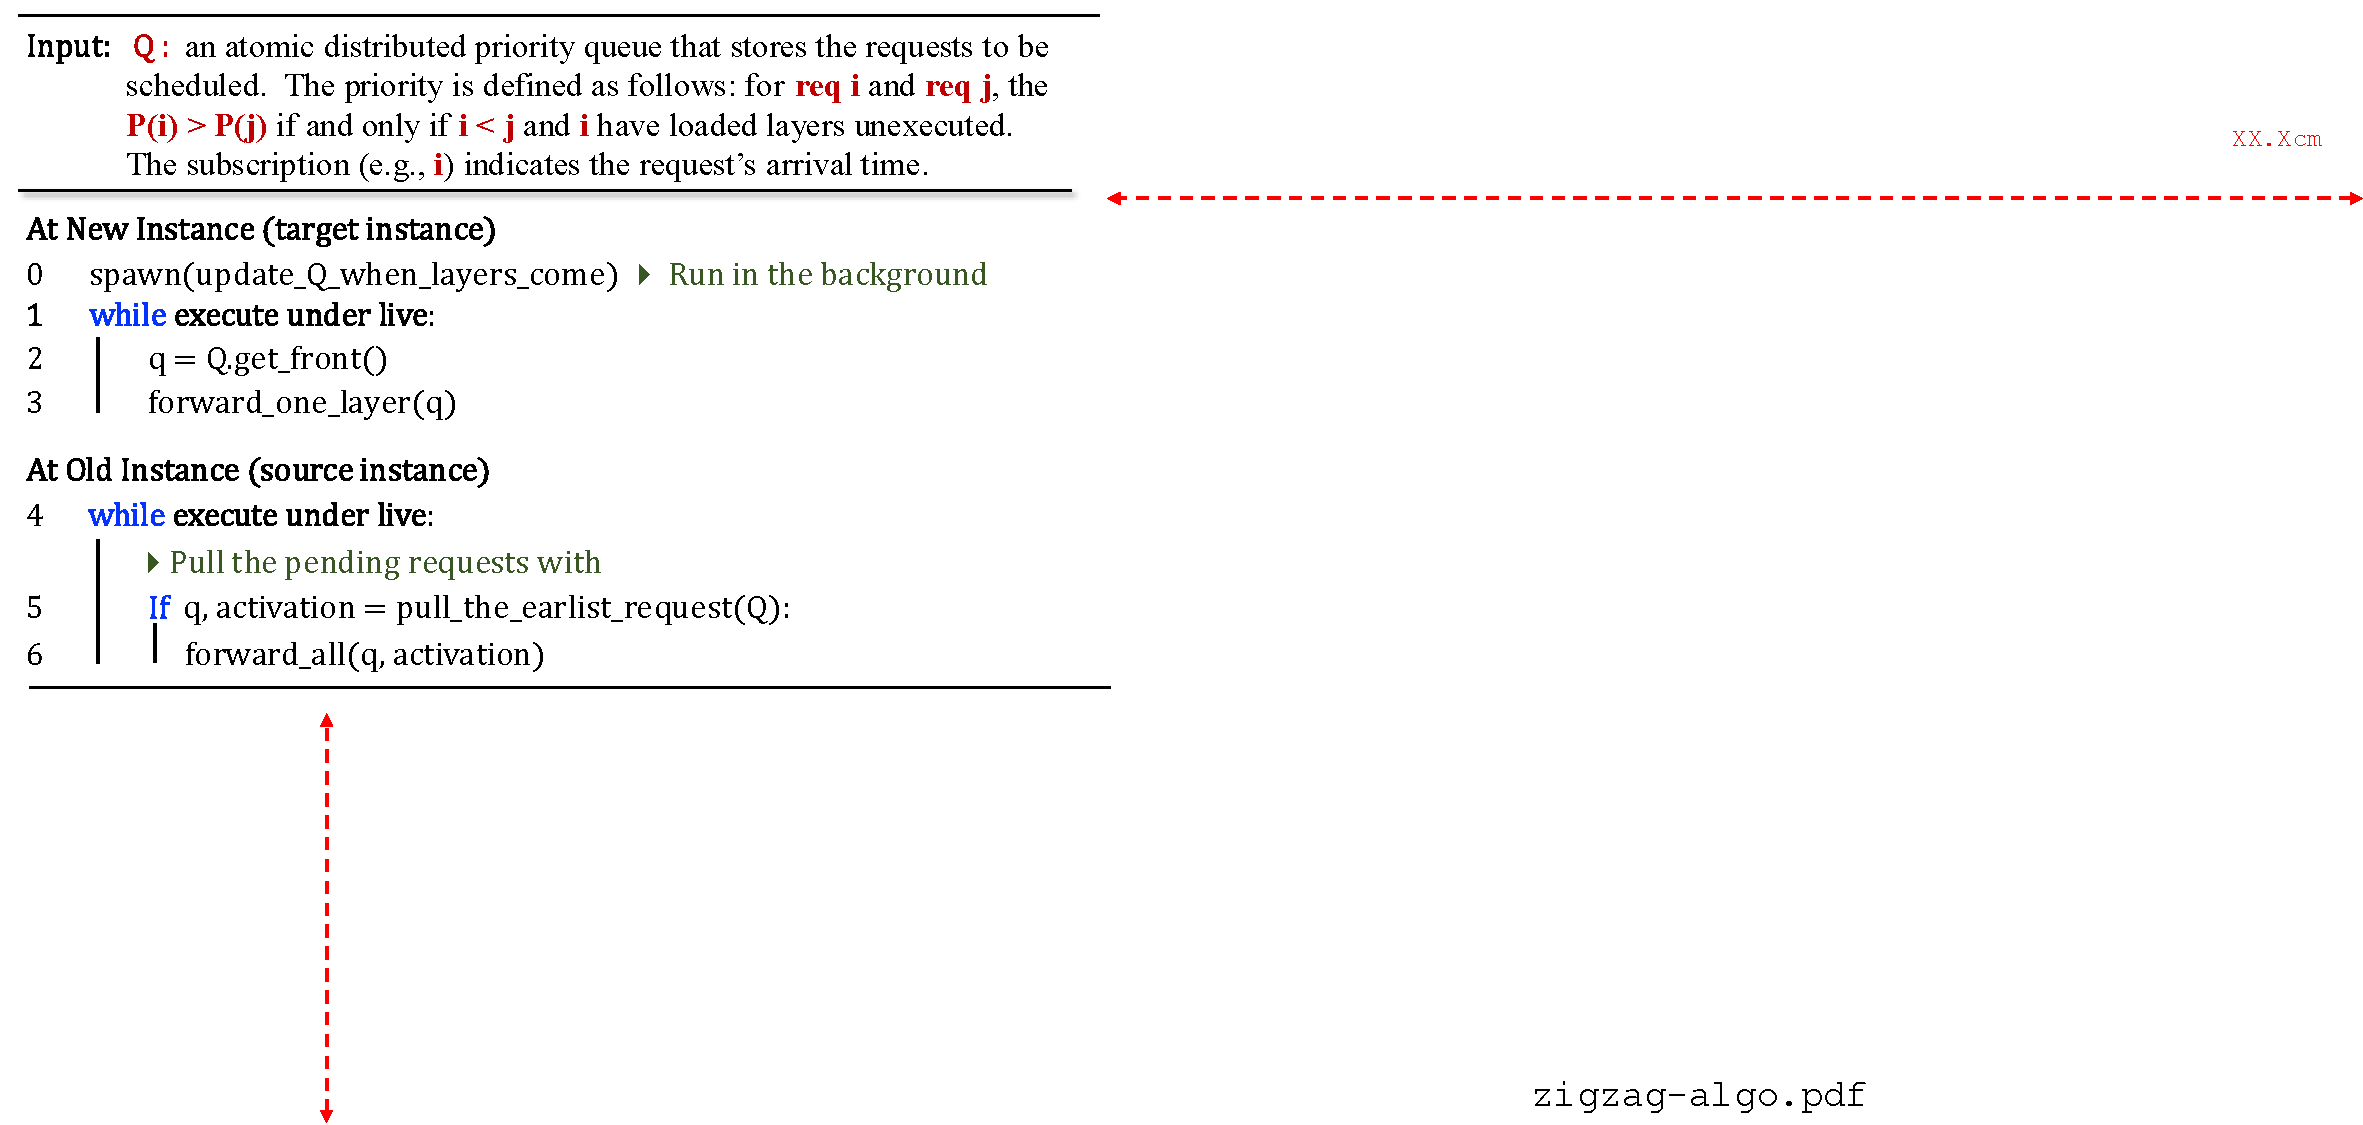
\includegraphics[width=1\textwidth, trim=0.25cm 6.99cm 21.3cm 0.25cm, clip]{figs/zigzag-algo.pdf} \\[1pt]
    \end{minipage} \\[3pt]
    \begin{minipage}{1\linewidth}
        \caption{\small{\textit{
            无需 ILP 的 ZigZag 调度伪代码。
        }}}
        \label{fig:zigzag-algo}
    \end{minipage} \\[-15pt]
\end{figure}

\emph{\textbf{(2) 以无 ILP 的 ZigZag 方式调度请求。}}
我们发现，
如果在源实例上适当延迟发送请求，
并让目标实例在其空闲时优先执行这些请求，
那么无需显式求解 ILP，也能达到 ZigZag 调度的效果。
{\fig{fig:zigzag-algo}} 给出了在两个实例上调度请求的伪代码。
新实例维护一个请求优先队列（源实例可以通过 RPC 拉取），
优先级由两部分决定：
(1) 请求在 FCFS 中的先后顺序；
(2) 下一层所需参数已经加载完成的请求优先。
一旦新实例执行完某个请求的一层（第 3 行），
该请求仍然会保留在队列中，
以便在后续更多层被加载后再次被调度回来执行。
而源实例只有在自己不再过载、也就是没有待处理请求时，
才会执行该请求（第 5 行）。
因此，只要源实例仍然繁忙，
请求就会继续留在目标实例侧执行。

\subsection{全局参数池与扩缩策略}
\label{sec:design-others}

\nospacestitle{全局参数池与本地内存缓存。 }
我们的全局参数池负责追踪模型参数在已部署 GPU 与主机 CPU 本地内存中的位置。
为了保证在整个集群范围内，
每个模型的参数至少在某张 GPU 或某台主机内存中保留一份副本，
在系统初始化时，
我们会把每个模型的一份参数均匀分散到各个 CPU 主机上，
并由一个中心化管理器记录这些副本的位置。
当模型被部署到某个 GPU 上，或从 GPU 上回收时，
我们会同步更新该管理器中的位置信息，
并相应回收或重新加载主机缓存中的副本。

\stitle{扩缩策略。\,}
本文聚焦于自动扩缩容机制本身，
它与扩缩策略是正交的；
后者包括如何收集工作负载指标，
以及基于这些指标决定要扩出多少新实例。
我们当前的实现遵循已有工作~\cite{DBLP:conf/osdi/SunHZXZL024,K8S-HPA}，
在全局范围内记录服务负载（以 tokens per second 和 KVCache 占用为指标）。

对于扩容，
当平均监控负载超过预先设定的上界时，
我们就分配足够多的实例去满足该需求。
这个上界可以通过离线 profiling 单实例平均服务能力得到。
更详细的策略说明我们放在另一篇论文中。
对于缩容，
我们沿用已有工作的基于超时策略~\cite{DBLP:conf/usenix/Romero0YK21,DBLP:journals/corr/abs-2401-14351}：
当一段时间窗口内平均负载低于下界时，
我们便关闭部分实例并收回其占用的 GPU。
由于 {\sys} 的自动扩缩速度非常快，
我们可以把这一超时时间设置得非常短，达到亚秒级。

\subsection{面向 LLM 的特化与优化}
\label{sec:design-llm}

\noindent
尽管前述大部分技术对所有遵循逐层架构的模型都适用，
但 LLM，尤其是采用 PD 解耦服务的 LLM，
仍然具有一些需要专门适配的特性。

\stitle{修正后的在线流水线调度公式。\,}
\textsection{\ref{sec:design-pp}} 中给出的公式与约束不能直接套用到 LLM，
因为在 LLM 中，一层的 prefill 时间与 decode 时间通常近似线性地依赖于 batch 中 token 的总数~\cite{DBLP:conf/isca/PatelCZSGMB24,DBLP:journals/corr/abs-2404-09526}。
对于只涉及 prefill 的在线调度场景——例如在 PD 解耦中对 prefill 实例进行扩缩——
我们通过为每个请求批次引入一个正则化参数来修正该公式，
该参数通过 profiling 请求批次在不同 token 数下的执行时间得到，
这一点与已有工作~\cite{DBLP:journals/corr/abs-2404-09526} 类似。
更棘手的是涉及 decode 的场景，
例如扩一个同时承担 prefill 与 decode 的实例，
或者在 PD 解耦中扩一个 decode 实例。
这是因为 decode 的 batch size 会由于自回归生成过程而不断变化。
幸运的是，
我们提出的无 ILP 调度方法同样适用于 decode 场景。

\stitle{支持 PD 共置（PD colocation）。\,}
我们可以无缝支持 PD 共置，
因为一个 PD 共置实例本质上就是一个普通模型实例。
与此同时，
我们的无 ILP ZigZag 调度同样适用于 PD 共置下的流水线执行~\cite{298679}。

\stitle{在 PD 解耦中在线扩缩 decode 实例。 }
在 PD 解耦场景下，
如果直接对 decode 实例做在线扩缩，
参数加载与 KVCache 传输都会形成入向流量，
从而在带宽上发生冲突，因此无法做到无干扰。
对此，我们利用一个事实：
prefill 实例与 decode 实例共享同一份模型参数。
因此，我们可以先把部分 prefill 实例转换成 decode 实例，
从而实现 decode 侧的在线扩缩；
与此同时，再对 prefill 实例执行在线扩缩，
以补偿 prefill 吞吐的损失。

\stitle{面向 PD 解耦的优化扩缩策略。\,}
提前扩实例（pre-scaling）能够隐藏扩缩开销，
但如果扩得过早，又会浪费 GPU 资源。
在 PD 解耦场景下，
我们发现可以以几乎零额外成本提前扩 decode 实例，
因为 decode 实例即将扩容的需求，
通常可以从 prefill 实例的扩容需求中推断出来。
具体来说，一旦我们检测到 prefill 实例存在明显扩容需求，
就会同步扩出对应的 decode 实例。
这种做法能够有效隐藏 decode 实例的扩缩开销，
而且对 ServerlessLLM~\cite{DBLP:journals/corr/abs-2401-14351} 这类其他系统同样有效，
详见 \textsection{\ref{sec:eval-app}}。

\section{评估}
\label{sec:eval}

\nospacestitle{系统实现。 }
{\sys} 是一个既能服务传统模型、也能服务 LLM 的 {\maas} 系统，
共包含约 24,000 行 Rust 与 C++ 代码。
它建立在 Prefill/Decode 解耦、continuous batching 等广泛使用的 LLM 优化之上。
在实现过程中，
我们尽可能复用现有的高性能服务系统组件（这些组件本身不具备自动扩缩容能力）。
例如，
我们所有用于 LLM 的 GPU kernel 都来自 FlashInfer~\cite{flashinfer}。
我们之所以选择基于原生语言的实现框架，
是因为我们发现用 Python 实现细粒度调度比较困难。
更多实现细节见 \textsection{\ref{sec:appendix}}。

\begin{table}[!t]
    \centering
    \small{
        \resizebox{.97\linewidth}{!}{
            \ra{1.2}
            \begin{tabular}{lrr} \toprule
                                 & \textbf{集群 A} ($m$ x $g$) & \textbf{集群 B} ($m$ x $g$) \\ \hline
                GPU              & A800 80\,GB (4x8)   & A100 80\,GB (2x8) \\
                GPU-GPU（机内）  & 1.6\,Tbps NVLink    & 256\,Gbps PCIe    \\
                GPU-GPU（机间）  & 100\,Gbps RDMA      & 100\,Gbps RDMA    \\
                Host-GPU         & 128\,Gbps PCIe      & 128\,Gbps PCIe    \\
                SSD-GPU          & 10\,Gbps            & 10\,Gbps          \\ \bottomrule
            \end{tabular}
        }
    } \\[8pt]
    \begin{minipage}{1\linewidth}
        \caption{\small{\textit{
        评估所使用的集群。$m$ 表示主机数量，$g$ 表示每台主机上的 GPU 数量。
        }}}
    \label{tab:cluster}
    \end{minipage} \\[-10pt]
\end{table}


\stitle{测试平台。 }
我们的实验在表~\ref{tab:cluster} 所示的两个测试平台上完成。
得益于 NVLink，
集群 A 更适合服务需要张量并行的大模型（如 72\,B）；
而集群 B 则更适合服务单 GPU 模型。

\stitle{评测轨迹与模型。 }
由于扩缩需求与请求到达率密切相关，
我们选择了三类典型的真实世界轨迹：
BurstGPT~\cite{wang2024burstgpt}，以及来自 Azure 的 AzureCode 与 AzureConv~\cite{DBLP:conf/isca/PatelCZSGMB24}。
这些轨迹的详细形状展示在 {\fig{fig:eval-e2e}} 的第一列中。
由于这些轨迹来自服务能力不同的集群，
我们遵循标准做法~\cite{DBLP:conf/asplos/MiaoSDXL0J24,DBLP:journals/pvldb/AliPYS22,DBLP:conf/osdi/GujaratiKAHKVM20}，
利用 TraceUpscaler~\cite{traceupscaler} 在保持时间模式不变的前提下缩放轨迹，
使其平均请求率约为我们集群最大服务能力的一半。

在模型方面，
我们重点评估 LLM，
因为其他非 LLM 模型更小，使用 {\sys} 进行扩缩几乎是轻而易举的。
具体来说，
我们选择了 Llama3-8B、Mistral-24B 与 Qwen2.5-72B，
它们都是当前流行且精度较高的 LLM。
由于 {\sys} 对模型规模更为敏感，
为了简化描述，后文在不引起歧义的情况下直接使用参数规模来指代模型。
其中，8\,B 模型每个实例仅需 1 张 GPU，
而 72\,B 模型的单实例至少需要 4 张 GPU。

\stitle{对比对象。\,}
在未特别说明时，
我们将 {\sys} 与以下基线系统进行比较：
\begin{enumerate}[leftmargin=*]
    \itemsep0.5em
    \setlength{\itemindent}{0em}
    \item \textbf{\emph{ServerlessLLM (S-LLM)
    ~\cite{DBLP:journals/corr/abs-2401-14351}}}
    是当前最先进、以提升自动扩缩速度为重点的 {\maas} 系统。
    它使用主机内存缓存最近加载过的模型，并采用基于 time-to-live 的淘汰策略。
    当缓存未命中时，
    它会以尽量打满 SSD 带宽的方式从 SSD 加载参数。 \\[-15pt]

    \item \textbf{\emph{ServerlessLLM optimal (AllCache)}}
    是 ServerlessLLM 的理想化版本，
    它总是能够从主机缓存中加载参数，因此在扩缩速度上是 ServerlessLLM 的上界。 \\[-15pt]

    \item \textbf{\emph{DistServe}}~\cite{DBLP:conf/osdi/ZhongLCHZL0024}
    是当前最先进的、但不支持自动扩缩容的 LLM 服务系统。
    它采用 PD 解耦。
    我们选择它作为对比对象，
    是因为在 PD 解耦场景中，多实例扩缩（prefill 与 decode）以及避免扩缩干扰都更具挑战性。
    我们将在 \textsection{\ref{sec:eval-pd-colocation}} 中，再与常见的 PD 共置系统（如 vLLM~\cite{vllm}）进行比较。 \\[-15pt]
\end{enumerate}

\noindent
为了保证公平，
我们为 {\sys} 与 S-LLM 的各个变体使用相同的扩缩策略。

\subsection{真实轨迹下的自动扩缩性能}
\label{sec:eval-app}

\begin{figure*}[!t]
    \centering
    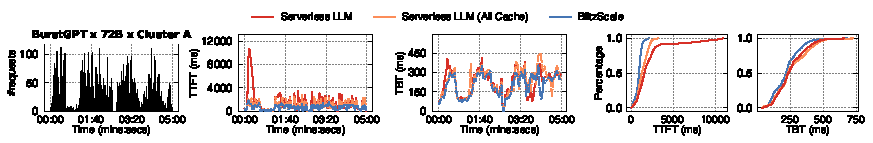
\includegraphics[width=1.01\textwidth,center]{./data/e2e-burstgpt.pdf} \\[0pt]
    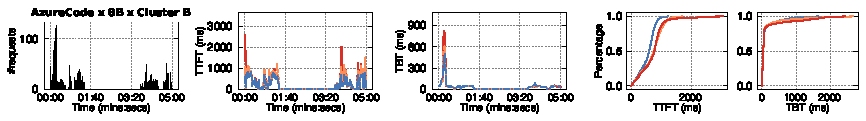
\includegraphics[width=1.01\textwidth,center]{./data/e2e-azurecode.pdf} \\[0pt]
    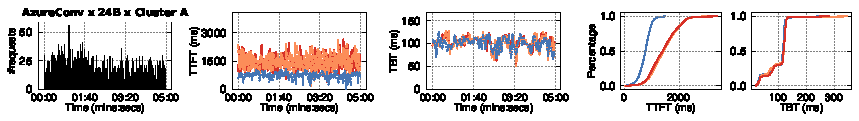
\includegraphics[width=1.01\textwidth,center]{./data/e2e-azureconv.pdf} \\[-5pt]
    \begin{minipage}{1\linewidth}
    \caption{\small{\textit{
        {\sys} 与 {\base} 在不同工作负载、模型与集群上的端到端性能对比。
    }}}
    \label{fig:eval-e2e}
    \end{minipage} \\[-10pt]
\end{figure*}

\noindent
受篇幅限制，
我们对每个模型只选择一个轨迹与一个集群进行展示。
{\fig{fig:eval-e2e}} 给出了在 prefill 与 decode 解耦、且两个阶段独立扩缩的设置下的端到端性能。
第一列展示轨迹的请求率，
第二列与第三列分别展示平均 TTFT 与平均 TBT，
其中每个点都是在 1 秒小时间窗内测得的平均时延；
最后两列则分别给出整个评测期间 TTFT 与 TBT 的累计分布函数（CDF）。
在本节中，
我们重点与 S-LLM 与 AllCache 比较；
由于 DistServe 不支持自动扩缩容，
我们将在下一小节单独与它比较。

\stitle{总体性能。 }
首先可以看到，
在所有工作负载上，{\sys} 的 TTFT 与 TBT 都是最低的，
这得益于其极快的自动扩缩速度。
具体而言，
在 BurstGPT 上，
{\sys} 的 TTFT 相比 S-LLM 与 AllCache 分别缩短了 75.5\,\% 与 21.1\,\%，
TBT 则分别缩短了 7.4\,\% 与 5.1\,\%。
不过，不同指标上的收益程度并不完全相同，
这是由 prefill 与 decode 阶段的不同特性共同决定的。
同时，
不同系统（尤其是 S-LLM）在不同工作负载下的行为也不一样，
这与它们的请求到达模式相关（见第一列）。
下面我们分别展开说明。

\stitle{TTFT 与 TBT 的差异。 }
在所有工作负载上，
{\sys} 对 TTFT 的改善都明显大于对 TBT 的改善。
这主要有两个原因。
第一，
借助我们优化后的策略（见 \textsection{\ref{sec:design-llm}}），
decode 实例可以被提前扩出，
而且我们对所有基线系统也采用了这一策略。
具体来说，
一旦 prefill 吞吐上升，
{\sys}（以及其基线）就会同步扩出 decode 实例，
因此在 decode 真正需要更多实例时，
扩缩时间已经与 prefill 阶段重叠，从而隐藏了一部分开销。
第二，
decode 的扩缩需求通常小于 prefill。
只要 decode 实例上的内存还足够，
所有系统通常都可以在几乎不产生排队的情况下处理 decode，
只是 TBT 会略有升高。
由于所有模型都采用了现代 LLM 优化中的 grouped-query attention~\cite{gqa}，
其显存占用较低，
因此 decode 侧通常比 prefill 侧更充裕。
尽管如此，
在三类工作负载上，{\sys} 的 TBT 相比 S-LLM 分别缩短了 5.1--7.4\,\%、88.3--94.1\,\% 与 0.7--1.8\,\%，
并且在各场景下也均优于 AllCache。

\stitle{不同工作负载之间结果差异。 }
借助高速网络扩缩与在线扩缩，
{\sys} 始终优于 AllCache；
但 S-LLM 相对 AllCache 的表现，则在不同工作负载之间有明显差异。
在 BurstGPT 上，
S-LLM 会在第一次突发（时间 0:05）出现显著 TTFT 尖峰，
但在之后的突发中与 AllCache 比较接近，
因为后续突发能够从主机缓存中获益。
相比之下，在 AzureCode 上，
S-LLM 在两次突发（时间 0:05 和 03:25）都会出现尖峰，
因为两次突发之间的间隔足够长，
导致主机缓存按照 TTL 策略被淘汰。
最后，在 AzureConv 上，
由于突发持续出现，S-LLM 基本总能命中主机缓存，
因此其性能——尤其从 CDF 图来看——与 AllCache 比较接近。

\subsection{性能与资源使用}
\label{sec:eval-resource}

\begin{figure*}[!t]
    \centering
    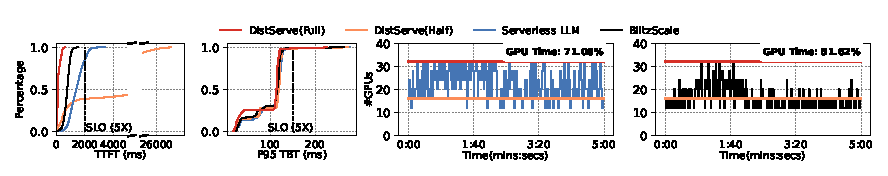
\includegraphics[width=1.01\textwidth,center]{./data/e2e-comparision-utilization-new.pdf}  \\[-10pt]
    \begin{minipage}{1\linewidth}
    \caption{\small{\textit{
        在 AzureConv 与 Mistral\,24B 组合下的 GPU 使用对比。
    }}}
    \label{fig:eval-e2e-gpu}
    \end{minipage} \\[-15pt]
\end{figure*}

\nospacestitle{与不支持自动扩缩容系统的比较。 }
我们首先将 {\sys} 与 DistServe 进行比较。
由于 DistServe 不支持自动扩缩容，
其性能高度依赖于预先分配的实例数量。
因此，我们评估两个设置：
DistServe (full) 使用整个集群的全部 GPU，
代表一种以浪费 GPU 为代价换取最佳性能的理想化配置；
DistServe (half) 则只使用在整个评测期间平均足以承载工作负载的实例数。
为简单起见，
这里我们只展示 AzureConv 上 24\,B 模型的结果，
整体趋势在其他设置中类似。
我们已经仔细校准了 DistServe 的性能，
确保在关闭 {\sys} 自动扩缩容后，
DistServe 与 {\sys} 在所有设置下表现一致。

{\fig{fig:eval-e2e-gpu}} 的前两列给出了时延结果。
首先可以看到，
DistServe (full) 的性能最好，
因为其 GPU 过度预配，不会遭受排队或扩缩开销。
尽管如此，
{\sys} 仍然在达到与 DistServe (full) 相同 SLO 的同时运行，
而 S-LLM 则有 18.7\,\% 的请求违反 SLO。
这里我们采用传统的 5\,$\times$ SLO~\cite{DBLP:conf/osdi/ZhongLCHZL0024}，
因为我们的工作负载（聊天与代码生成）都属于时延敏感型。
也就是说，
若某个请求的端到端 TTFT 或 TBT 超过平均时延的 5\,$\times$，
就视为违反 SLO。
最后，DistServe (half) 的性能最差：
平均来看，{\sys} 的 TTFT 与 TBT 分别比 DistServe (half) 短 95.8\,\% 与 1\,\%。
而做到这一点的同时，
{\sys} 用于服务该模型的 GPU 时间与 DistServe (half) 相同，
并且仅为 DistServe (full) 的一半。
下面我们进一步说明这一点。

\stitle{GPU 时间消耗。\,}
{\fig{fig:eval-e2e-gpu}} 的最后两列分别展示了 S-LLM 与 {\sys} 的 GPU 时间消耗。
对于 S-LLM 与 {\sys}，
我们分别收集每个时刻所有 prefill 与 decode 实例的聚合 GPU 使用量，
然后对曲线下方面积进行积分，得到整体 GPU 时间。
对于 DistServe 的两个变体，
其 GPU 时间在整个评测期间是常数。
结果表明，
得益于更快的自动扩缩速度，{\sys} 的 GPU 时间比 S-LLM 低 19.46\,\%。
当扩缩速度较慢时，
队列中会积压更多请求，
系统因而会触发更多扩缩动作，
最终消耗更多 GPU 时间。
而 {\sys} 则避免了这种额外消耗。
即便使用了更少的 GPU 时间，
{\sys} 的 TTFT 与 TBT 仍分别比 S-LLM 短 48.1\,\% 与 1.8\,\%。

\begin{figure}[!t]
    \centering
    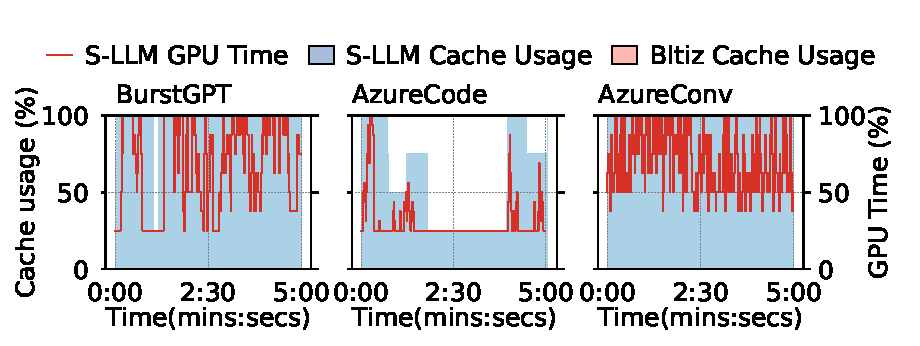
\includegraphics[width=1.0\linewidth,center]{./data/motiv-cache-usage-new.pdf}  \\[2pt]
    \begin{minipage}{1\linewidth}
    \caption{\small{\textit{
        在评测工作负载下，S-LLM 与 {\sys} 的主机缓存使用对比。
    }}}
    \label{fig:eval-cache-usage}
    \end{minipage} \\[-20pt]
\end{figure}

\stitle{主机缓存使用。\,}
与 ServerlessLLM 相比，
{\sys} 用于参数缓存的主机内存也更少。
{\fig{fig:eval-cache-usage}} 给出了不同系统的主机内存使用情况。
我们省略了 AllCache 与 DistServe：
前者始终会把参数完全复制到所有主机上，
后者则完全不需要缓存。
由于不同工作负载使用的集群不同，
我们对主机缓存使用量做了归一化。
这一结果传递了两个信息。
第一，{\sys} 仅需极少量的主机缓存（不到 1 份副本）就能实现快速自动扩缩容。
这与我们的设计一致：
我们优先从已经服务该模型的实例 GPU 上加载参数；
而即使当前没有任何服务实例，
借助基于网络的多播，我们也只需要 1 份主机缓存副本。
第二，ServerlessLLM 的内存使用与参与服务的主机数量成正比，
因此某个模型会迅速“污染”主机缓存。
对于一个同时服务很多模型、且主机缓存有限的 {\maas} 系统来说，
这种做法显然并不理想。

\subsection{更细粒度的性能分析}
\label{sec:eval-ablation}

\begin{figure*}[!t]
    \centering
    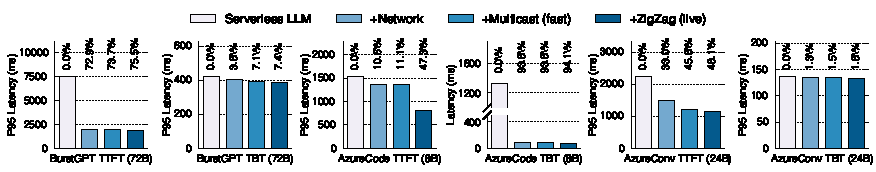
\includegraphics[width=1.01\textwidth,center]{./data/abl-new.pdf}  \\[-2pt]
    \begin{minipage}{1\linewidth}
    \caption{\small{\textit{
        对本文提出技术有效性的消融实验。
    }}}
    \label{fig:eval-alb}
    \end{minipage} \\[-20pt]
\end{figure*}

\begin{figure}[!t]
    \centering
    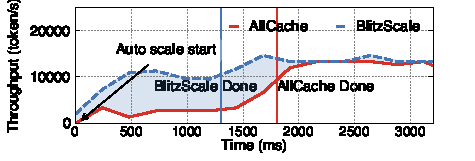
\includegraphics[width=1.0\linewidth,center]{./data/ext.pdf}  \\[2pt]
    \begin{minipage}{1\linewidth}
    \caption{\small{\textit{
        在集群 A 上把一个 24\,B 模型扩到 6 个 prefill 实例时，{\sys} 与 AllCache 的扩缩细节对比。
    }}}
    \label{fig:scale-breakdown}
    \end{minipage} \\[-5pt]
\end{figure}

\nospacestitle{在线扩缩的细节观察。 }
{\fig{fig:scale-breakdown}} 展示了使用 {\sys} 与 AllCache 把一个 24\,B prefill 模型扩到 6 个实例时的吞吐时间线。
{\sys} 使用了两条广播链（每条链覆盖 3 个实例），
其中链尾实例采用在线扩缩；
两条链的起始节点则是 decode 实例。
对于 AllCache，
它直接从新扩实例所在主机的内存中加载参数。
我们可以看到：
第一，哪怕只加载了很少的层（例如在 500\,ms 时），
{\sys} 也已经能够由于在线执行而逐步输出 token。
第二，借助基于 NVLink 的融合链路传输协议，
{\sys} 的扩缩速度甚至比 AllCache 更快：
它可在约 1,200\,ms 内完成扩缩，而 AllCache 约需 2,000\,ms。

\stitle{消融实验。 }
{\fig{fig:eval-alb}} 对我们提出技术的有效性进行了消融分析。
评估方式是逐步开启不同技术，并观察三种工作负载上的效果：
“+Network” 表示扩缩时使用高速计算网络而不是 SSD；
“+Multicast (fast)” 表示进一步采用 \textsection{\ref{sec:design-plan}} 中介绍的优化广播协议；
“+ZigZag (live)” 表示启用 \textsection{\ref{sec:design-pp}} 中的在线自动扩缩容机制。

首先可以看到，
所有技术都能提升端到端服务性能，
只是不同工作负载下收益大小不同。
“+Network” 在所有工作负载上都有效，
因为它为扩缩容数据平面提供了更高带宽。
“+Multicast (fast)” 在 AzureCode 与 AzureConv 上效果明显，
但在 BurstGPT 上收益较小，
这是因为受限于我们的集群规模，
在 72\,B 模型上最多只能同时扩 8 个实例，
因此几乎不存在“同时扩多个实例”的场景，
而这正是多播优化最擅长的场景。
在线自动扩缩容主要在 AzureCode 上最有效，
因为它是在网络更慢的集群 B 上评测的。
最后，
我们的方法在 decode 阶段上的收益通常不如 prefill 明显，
因为大多数情况下 decode 实例已经足够充足，
这一点我们已在 \textsection{\ref{sec:eval-app}} 中讨论过。
一个例外是 AzureCode：
在该工作负载中，prefill 吞吐增长得比其他负载更慢（见 {\fig{fig:eval-e2e}} 第一列），
因此 decode 实例的扩容会被更晚触发。
这使得 ServerlessLLM 的 SSD 慢扩缩无法被隐藏，
从而使更快的扩缩方式显得更有价值。

\begin{figure}[!t]
    \centering
    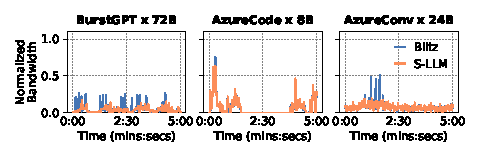
\includegraphics[width=1.0\linewidth,center]{./data/network-util.pdf}  \\[-10pt]
    \begin{minipage}{1\linewidth}
    \caption{\small{\textit{
        {\sys}（Blitz）的网络使用情况分析。
    }}}
    \label{ffig:eval-network-util}
    \end{minipage} \\[-10pt]
\end{figure}

\stitle{网络使用。 }
{\fig{ffig:eval-network-util}} 展示了 {\sys} 与 S-LLM 的网络使用情况。
可以看到，
尽管 {\sys} 利用计算网络执行自动扩缩，
而且扩缩频率也较高（见 {\fig{fig:eval-e2e-gpu}} 最后一列），
但其带来的额外网络开销仍然可以忽略不计。

\begin{figure}[!t]
    \centering
    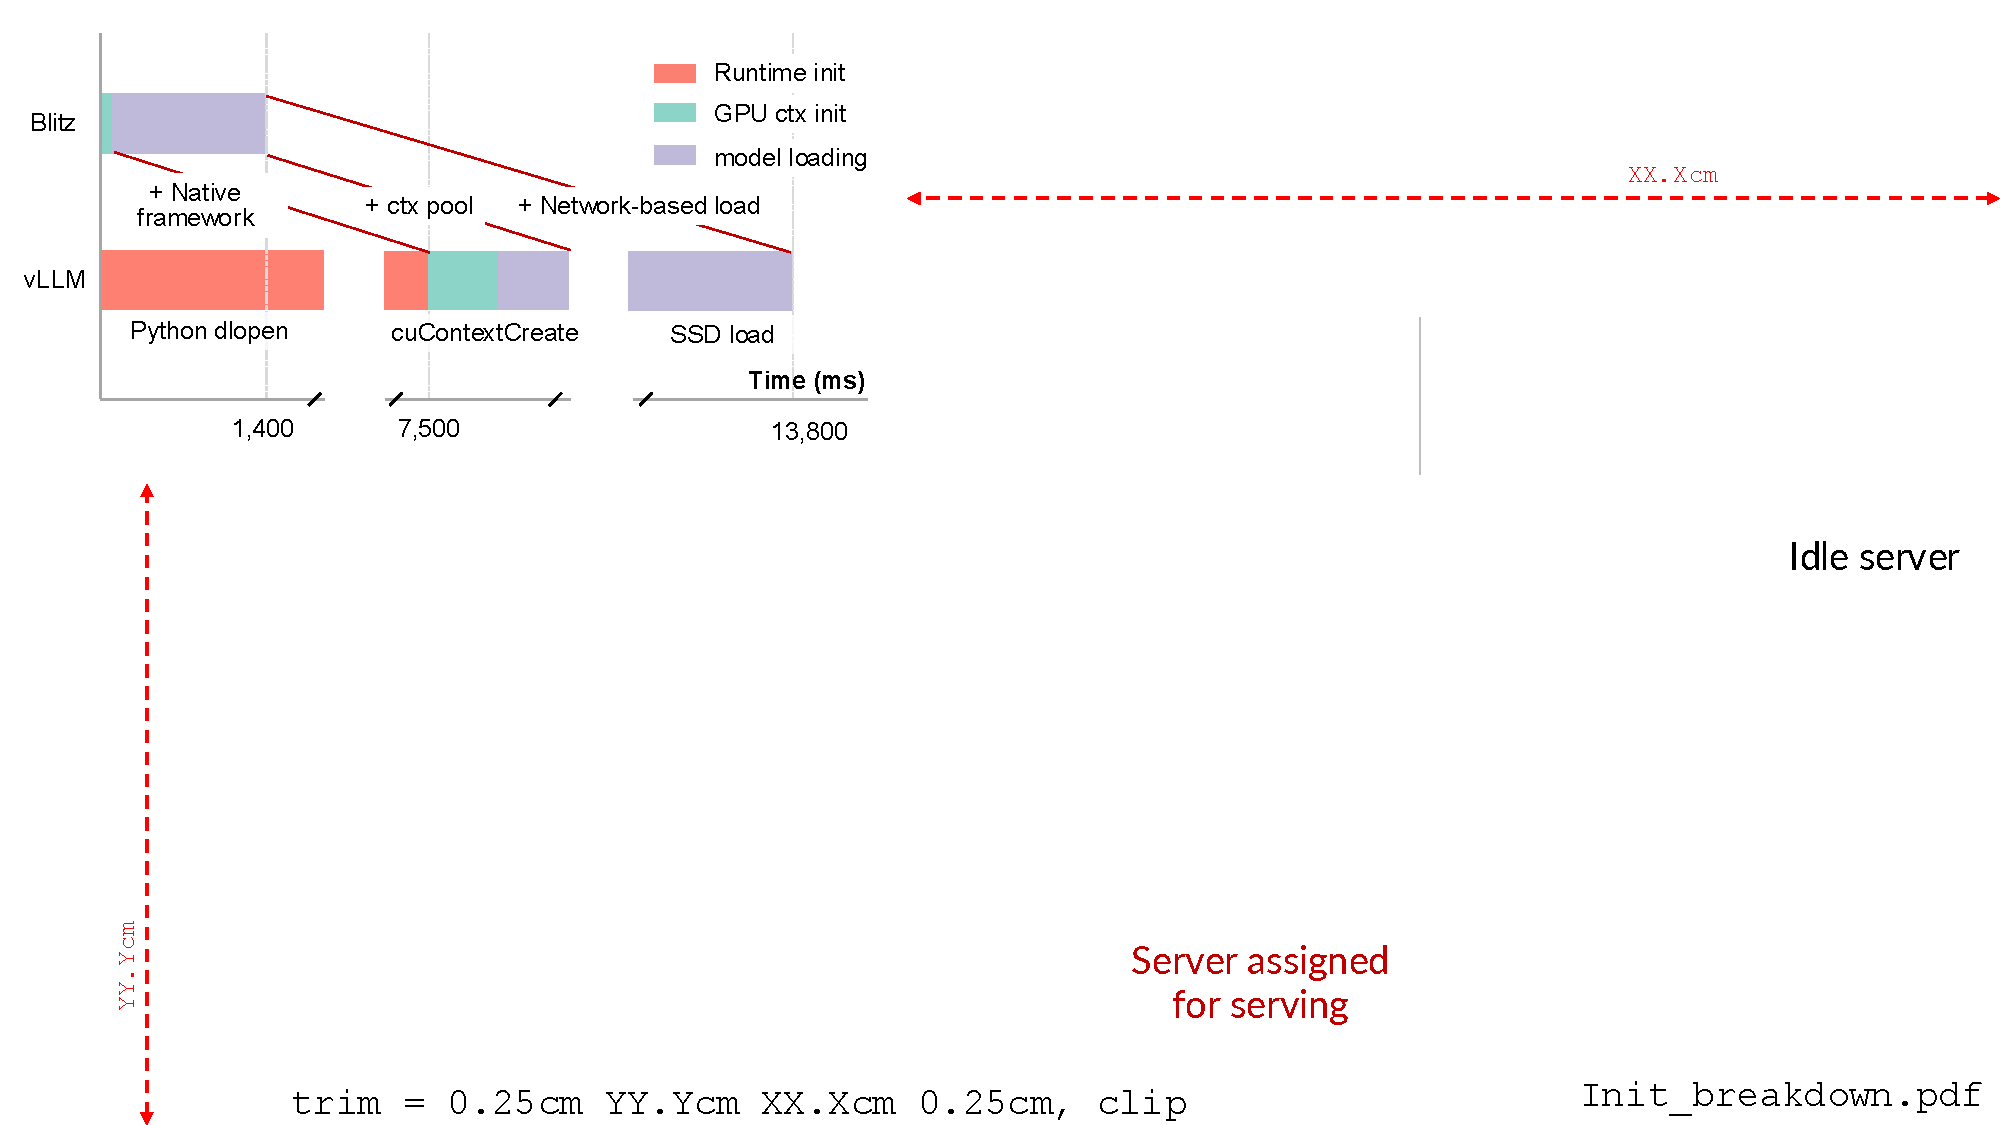
\includegraphics[width=.95\columnwidth, trim=0.25cm 10.9cm 18.55cm 0.9cm, clip]{figs/init_breakdown.pdf}
    \\[-8pt]
    \begin{minipage}{1\linewidth}
    \caption{\small{\textit{
        {\sys} 与 vLLM 的初始化时间对比。
    }}}
    \label{fig:breakdown}
    \end{minipage} \\[-10pt]
\end{figure}

\stitle{模型自动扩缩容中的控制平面与数据平面。 }
{\fig{fig:breakdown}} 将 {\sys} 与 vLLM 在自动扩缩时的控制平面和数据平面开销进行了对比。
结果表明，只要实现得当，
控制平面开销几乎可以忽略。

\subsection{LLM 的 PD 共置场景性能}
\label{sec:eval-pd-colocation}

\begin{figure}[!t]
    \centering
    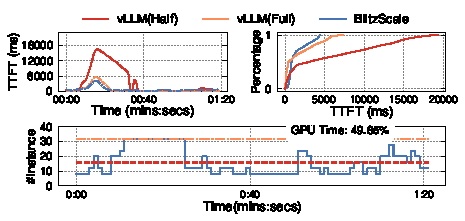
\includegraphics[width=1.0\linewidth,center]{./data/e2e-collocation-burstgpt.pdf}  \\[2pt]
    \begin{minipage}{1\linewidth}
    \caption{\small{\textit{
        {\sys} 与 vLLM 在 BurstGPT 工作负载上的对比。
    }}}
    \label{fig:eval-colocation}
    \end{minipage} \\[-10pt]
\end{figure}

\noindent
最后，{\fig{fig:eval-colocation}} 比较了 {\sys} 与 vLLM 在 PD 共置设置下的性能，
此时服务运行在 BurstGPT 工作负载与 Llama2-7B 模型上。
整体趋势与 PD 解耦场景类似：
{\sys} 的性能与过度预配的 vLLM 相当；
而与按平均需求预配的 vLLM 相比，
{\sys} 的 P99 TTFT 可缩短到其 0.24\,$\times$。
更有意思的是，
我们发现 {\sys} 的尾部 TTFT 甚至比过度预配的 vLLM 还更短，
这是因为我们的调度框架是针对集群级服务优化设计的。

\section{相关工作}
\label{sec:related}

\nospacestitle{无自动扩缩容条件下的模型服务优化。 }
大规模模型服务并不简单。
大量研究关注如何高效利用 GPU 来加速模型服务~\cite{DBLP:conf/osdi/ZhongLCHZL0024,DBLP:journals/corr/abs-2404-09526,vllm,alpaserve,DBLP:conf/osdi/YuJKKC22,DBLP:conf/isca/PatelCZSGMB24,298501,kvcache}。
例如，Orca~\cite{DBLP:conf/osdi/YuJKKC22} 提出了迭代式调度与选择性批处理；
AlphaServe~\cite{alpaserve} 采用流水线并行来更好地应对负载尖峰，
但它无法动态调整流水线实例。
这些系统都假设运行在固定规模的 GPU 池上，
而我们已经说明了动态调整池规模的必要性，
并展示了如何通过 {\sys} 高效实现这一点。
{\sys} 为这些单实例模型服务系统补充了快速自动扩缩容机制：
我们建立在它们的高效单实例服务能力之上，
并在系统需要改变服务实例数量时提供超快扩缩容。

\stitle{动态扩缩服务实例。 }
动态扩缩服务实例的难点主要在于模型权重体积巨大且仍在持续增长，
因此把它们加载到加速器上（数据平面）十分耗时。
已有一些工作尝试加速该加载过程~\cite{pipeswitch, DBLP:conf/eurosys/JeongBA23, DBLP:conf/asplos/MiaoSDXL0J24, DBLP:conf/osdi/SunHZXZL024}。
例如，PipeSwitch~\cite{pipeswitch} 和 DeepPlan~\cite{DBLP:conf/eurosys/JeongBA23}
都利用模型逐层执行的特性，把推理与参数加载重叠起来以隐藏加载开销。
但它们只关注主机到设备的加载，而且当模型较大时，这种重叠仍然不是在线式的。
SpotServe~\cite{DBLP:conf/asplos/MiaoSDXL0J24} 与 Llumnix~\cite{DBLP:conf/osdi/SunHZXZL024}
实现了在线迁移，但迁移无法完全释放新旧两个实例的计算能力。
{\sys} 提供了一种新的机制，使服务实例在参数加载过程中也能在线扩缩，
即使加载尚未完成也能提升吞吐，
而我们已证明这对降低突发负载下的延迟至关重要。

并发工作 $\lambda$Scale~\cite{yu2025lambdascale} 也关注利用网络加速模型自动扩缩容。
关键区别在于，$\lambda$Scale 会把一次扩缩涉及的参数分散到多个实例上，
以降低扩缩时间，但代价是服务吞吐下降；
而 {\sys} 则可以以相近速度把完整参数无缝扩到所有实例上，
并借助基于多播链的扩缩过程避免牺牲吞吐。
此外，{\sys} 在扩缩过程中由于在线扩缩而具备逐步上升的吞吐，
而 $\lambda$Scale 仍然属于 stop-the-world 方法。

\stitle{加速无服务器计算中的冷启动。 }
加速模型扩缩容与无服务器计算中的冷启动加速一脉相承~\cite{sock,sand,FAASM,DBLP:conf/asplos/DuYXZYQWC20,DBLP:conf/asplos/Ustiugov0KBG21,DBLP:conf/eurosys/SaxenaJSKA22,DBLP:conf/usenix/WangCTWYLDC21}，
后者关注如何启动容器等通用计算实例。
我们继承了这些工作的思路，例如用于加速容器启动时间，
但进一步针对模型服务这一领域，结合其特定知识，
设计了高效的基于网络的在线自动扩缩容机制。

\section{结论与未来工作}
\label{sec:concl}

\noindent
在模型即服务系统中，自动扩缩容是同时实现高有效吞吐和高硬件利用率的关键，
但现有自动扩缩容机制既慢又是 stop-the-world，
其带来的性能开销显著限制了实际效果。
本文首先表明，借助基于网络、面向模型的多播，
模型自动扩缩容的数据平面可以在少于 $O(1)$ 缓存的条件下做到快速；
随后我们进一步说明，借助面向模型的远程执行，
数据平面还可以做到在线。
结合这两项技术后，
与当前最先进的、分别支持和不支持自动扩缩容的服务系统相比，
{\sys} 最多可带来 94.1\,\% 的性能提升和 19.46\,\% 的资源利用率提升。
我们相信，这项工作展示了由自动扩缩容赋能的模型即服务系统所具备的潜力与可行性。

尽管 {\sys} 的快速在线自动扩缩容向现代弹性服务系统迈出了关键一步，
仍有若干挑战值得继续研究。
首先，在我们的研究中发现，
扩缩容策略——即何时扩缩、如何扩缩——同样会显著影响系统效率。
这类策略高度依赖工作负载特征，
我们将其留作未来工作。
其次，{\sys} 当前聚焦于实例级扩缩容，
而现代模型也可以通过改变实例内部的并行配置来扩缩，
例如对混合专家（MoE）模型中的专家进行扩缩。
原则上 {\sys} 也适用于这类场景，
但更细致的探索仍有待未来开展。

\section*{致谢}
\noindent
我们感谢 OSDI 评审人与 shepherd 提出的深刻反馈。
我们衷心感谢 Qinwei Yang、Xinhao Luo 和 Mingcong Han
在 GPU 通信库、内核、驱动与运行时方面给予我们的建议。
同时感谢 Xiating Xie、Chenhan Wang 和 Sundi Guan
帮助我们改进论文表述。
我们感谢阿里巴巴通义实验室在本工作早期阶段提供测试平台。
本研究部分得到以下项目支持：
国家重点研发计划（No. 2022YFB4500700）、
中央高校基本科研业务费、
国家自然科学基金（No. 62202291, 62272291），
以及华为云研究资助。


\balance

\small{
\bibliographystyle{acm}
\bibliography{fastllmstart}
}

\twocolumn
\appendix
\section{附录}
\label{sec:appendix}

\begin{table*}[!ht]
	\centering
	\begin{tabular}{lllllll}
		\toprule
		\textbf{实例类型} & \textbf{加速器} & \makecell{\textbf{本地 SSD}\\\textbf{带宽/GPU}} & \makecell{\textbf{远程 SSD}\\\textbf{带宽/GPU}} & \makecell{\textbf{网络}\\\textbf{带宽/GPU}} & \textbf{含 NVLink} & \textbf{价格} \\ \midrule
		a2-ultragpu-8g \cite{googleinstance}      & 8 x A100(80\,GB) & 2.58\,Gbps & 0.29\,Gbps & 12.5\,Gbps & \ding{51} & 40.44 USD/h \\
		p4d.24xlarge\cite{awsinstance}            & 8 x A100(40\,GB) & 2.31\,Gbps & -          & 100\,Gbps  & \ding{51} & 45.039 USD/h \\
		ml.hpcpni2.28xlarge\cite{volcanoinstance} & 8 x A100(80\,GB) & 4\,Gbps    & -          & 100\,Gbps  & \ding{55} & 48.23 USD/h \\
		p4de.24xlarge\cite{awsinstance}           & 8 x A100(80\,GB) & 2.31\,Gbps & -          & 100\,Gbps  & \ding{51} & 56.328 USD/h \\
		a3-highgpu-8g\cite{googleinstance}        & 8 x H100         & 6.09\,Gbps & 0.97\,Gbps & 100\,Gbps & \ding{51} & 88.25 USD/h \\
		a3-megagpu-8g\cite{googleinstance}        & 8 x H100         & 6.09\,Gbps & 0.97\,Gbps & 200\,Gbps & \ding{51} & 不可用 \\
		p5.48xlarge \cite{awsinstance}            & 8 x H100         & 9.8\,Gbps  & -          & 400\,Gbps  & \ding{51} & 不可用 \\ \bottomrule
	\end{tabular} \\[10pt]

    \begin{minipage}{1\linewidth}
        \caption{\small{\textit{
		来自 GPU 云厂商的 {\maas} 硬件配置概览。
        }}}
    \label{tab:vendor-hardware}
    \end{minipage}
\end{table*}

\subsection{值得说明的实现细节}
\label{sec:appendix-implementation}

\nospacestitle{网络库。 }
我们实现了一个通信库，
统一抽象 NVLink 和 RDMA，
从而整体性地完成参数传输，
这一点与 DeepEP~\cite{deepep} 类似。
在实现过程中我们发现，
如果直接使用现成的组通信器（例如 NCCL~\cite{nccl}），
跨机器建立通信组的开销较大（例如 100\,ms），
这会显著限制基于网络扩缩容的效果。
幸运的是，我们的计划只需要节点对之间的 P2P 通信。
因此，我们预先构建了一个连接池，
支持各节点之间的全互连连接。
尽管计算网络（RDMA）在可扩展性上存在潜在问题~\cite{fasst}，
但这主要出现在小负载传输场景中，
并且可以通过 DCT~\cite{krcore} 等先进 RDMA 传输机制来缓解。

\stitle{带 CUDA 上下文池的原生服务引擎。 }
在执行之前，GPU 上必须先创建一个带已加载内核（cuModule）的 CUDA 上下文。
创建这样一个 CUDA 上下文大约需要 500\,ms，
在服务实例自动扩缩容中不可忽略。
为降低该开销，{\sys} 维护了一个小规模 CUDA 上下文池，
其中预先加载好常用内核，
然后在已有 CUDA 上下文中把参数传入 GPU，
这一做法与已有工作~\cite{DBLP:journals/corr/abs-2405-12079} 类似。
此外，{\sys} 使用 C++ 与原生 CUDA API 构建，
从而消除了初始化 PyTorch（例如 \texttt{dlopen}）带来的额外开销。

\stitle{容错。 }
发生机器故障时，
我们会利用自身的扩缩容机制自动扩出新的实例。
其中一个问题是，故障机器上的缓存参数会一并丢失，
因此需要把这些参数重新分发到其他机器上，
以维持全局参数池的不变式。
对于调度器、监控器等其他组件的故障，
我们沿用现有工作中的恢复流程~\cite{DBLP:conf/usenix/Romero0YK21,DBLP:journals/corr/abs-2401-14351}。

\subsection{{\maas} 的硬件配置}
\label{sec:appendix-hardware}

\noindent
表~\ref{tab:vendor-hardware} 列出了典型 {\maas} 系统所依赖的硬件配置。


\clearpage
\end{document}
